% encoding: utf8
% !TEX encoding = utf8
% !TeX spellcheck = pl_PL

\chapter{Działanie systemu\label{chap:weryfikacja_systemu}}
\graphicspath{{../../velma/przerobione_testy/out/}{./images}}

Algorytm kompensacji grawitacji zaimplementowano modyfikujac komponent \textit{cart\_imp} odpowiedzialny za wyliczanie prawa sterowania oraz inne komponenty. W celu weryfikacji wymagań systemu zostal napisany program komunikujacy sie z agentem \textit{velma\_ros\_interface}. Program  nakazujacy robotowi manipulowanie chwytakiem w trybie sterowania impedancyjnego w przestrzeni operacyjnej uruchomiono w trybie symulacji. Program jest uruchamiany w trybie wysokiej i niskiej sprezystosci oraz z wlaczonym i wylaczonym algorytmem kompensacji grawitacji. W trakcie wszystkich eksperymentow wszystkie parametry algorytmu sterowania byly takie same. TODO: dodac osie w sekcji o robocie 

\section{Ocena jakosci sterowania}
Okreslenie jakosci algorytmu mozliwe jest dzieki modyfikacji komponentu \textit{TfPublisher}. Po modyfikacji udostepnia on dane o pozycji zadanej z interpolatora trajektorii oraz o pozycji osiagnietej. Ocena jakosci sterowania nastepuje poprzez porownanie wynikow obliczonych zgodnie z metryka APE opisanej w sekcji \ref{chap:ape}. W pracy nie zamieszczono wynikow dzialania algorytmu sterowania bez kompensacji i z chwyconymi przedmiotami poniewaz nie byly one w zadnym stopniu wykonywane. Testy polegaly na chwytaniu dwoch przedmiotow. Puszka ma wage ok 1 kg jest walcem z rowomiernie rozlozona masa. Wiertarka ma wage ok 1,5 kg i jej rozklad mas nie jest rownomierny.


\subsection{Ruch ósemkowy}

Eksperyment ma przetestowac zachowanie algorytmu kompensacji przy skomplikowanych ruchach (rys. \ref{fig:osemka_a}, \ref{fig:osemka_rot}).  Ruch "osemkowy" zadany jest w osi $Y$ oraz $Z$.
Trajektoria jest zadana zgodnie ze wzorem lemniskaty Bernoulliego opisanej wzorem:
\begin{equation}
(y^2 + z^2)^2 = 2a^2(y^2-z^2)
\end{equation}

gdzie:
\begin{itemize}
	\item $y$ oraz $z$ to wspolrzedne trajektorii
	\item $a$ to parametr rownania
\end{itemize}

Trajektoria ruchu w rzucie na wprost ruchu zostala zaprezentowana na rys. \ref{fig:osemka_porow_komp}, \ref{fig:osemka_porow_przedm} i \ref{fig:osemka_porow_zbiorcze_a}. Trajektoria widoczna z boku (w osiach $X$ oraz $Z$) zostala zaprezentowana na rys. \ref{fig:osemka_porow_komp_bok}, \ref{fig:osemka_porow_przedm_bok} i \ref{fig:osemka_porow_zbiorcze_b}.
\begin{figure}[h]
	\centering
	\subfigure[Os $X$]{
		\label{fig:osemka_ax}
		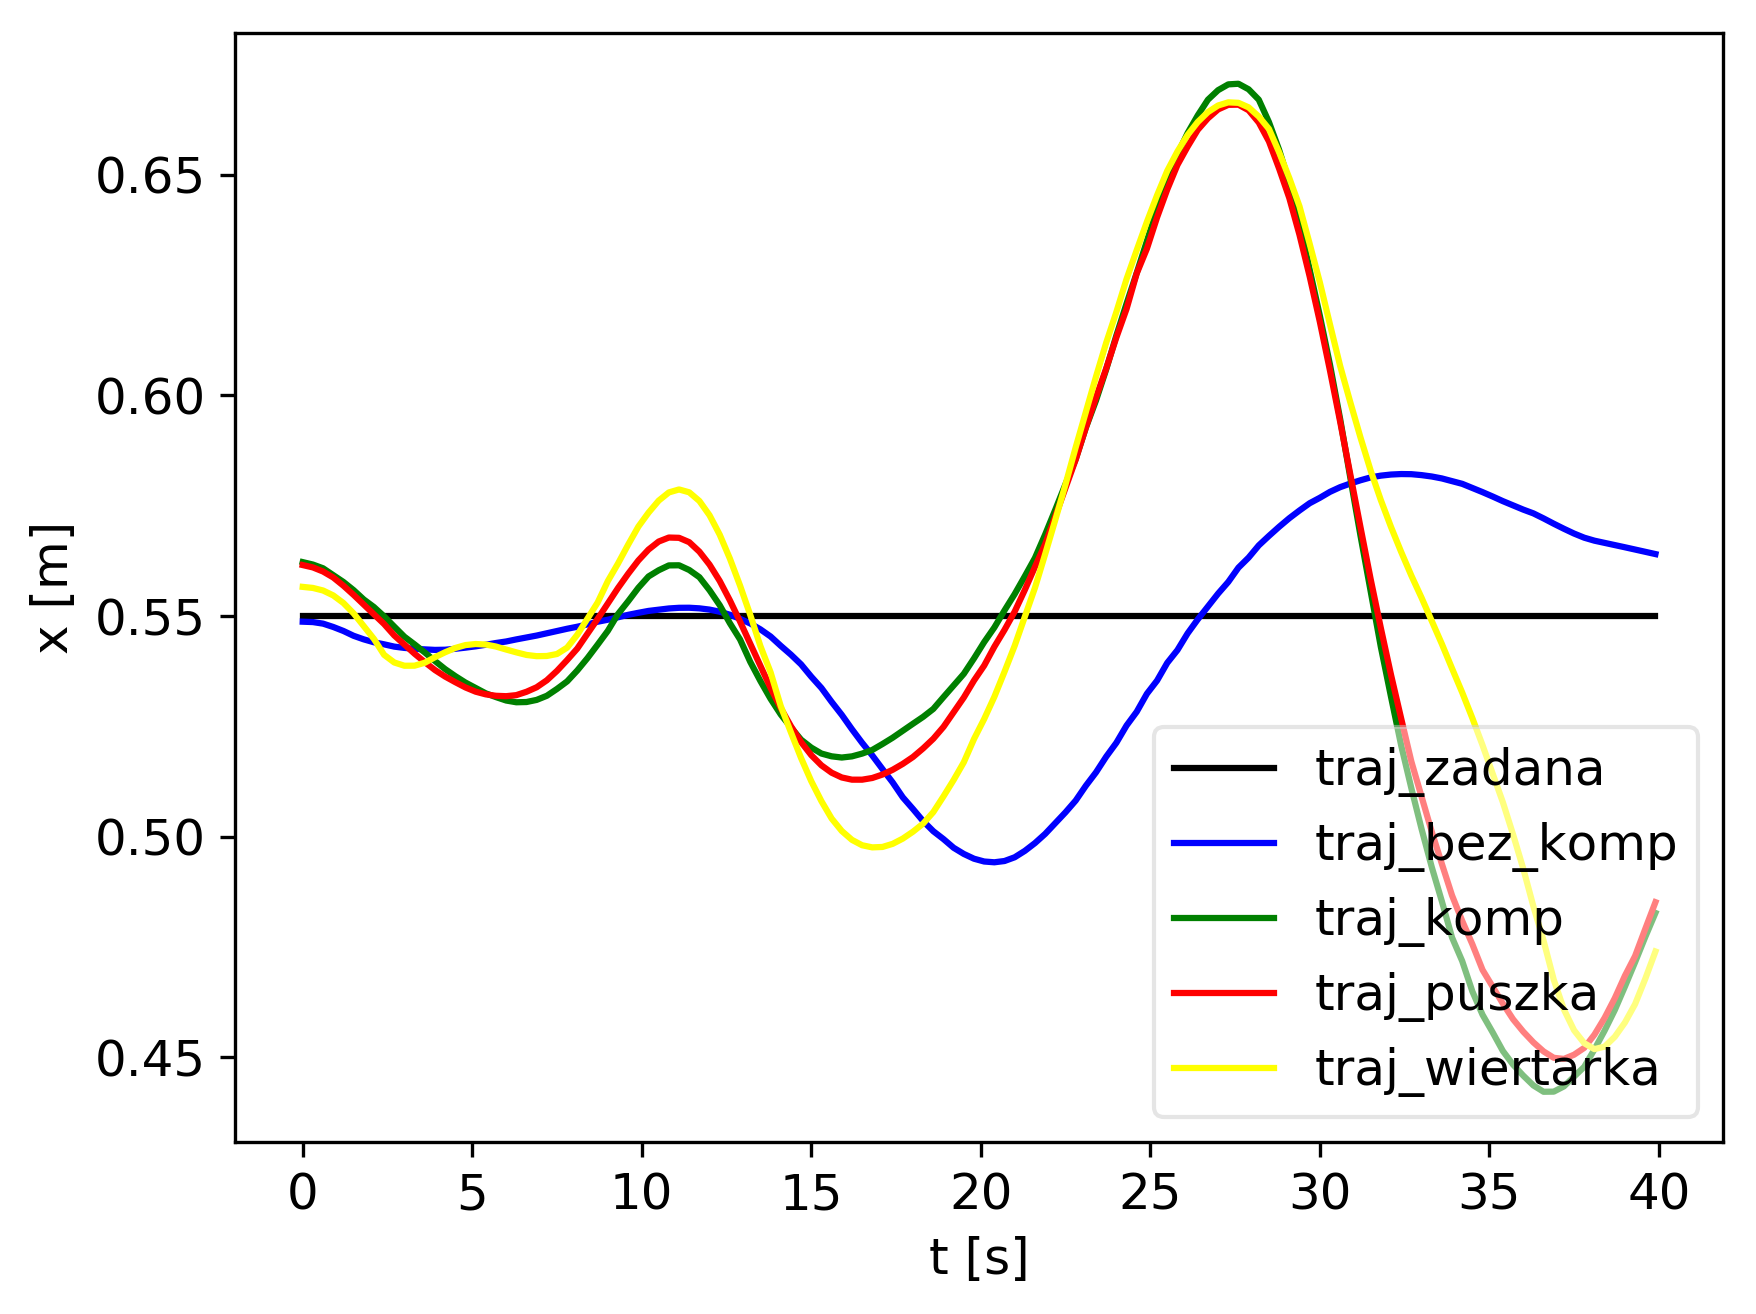
\includegraphics[width=.45\textwidth]{../../velma/przerobione_testy/out/osemka/common_ax.png}
	}
	\hfill
	\subfigure[Os $Y$]{
		\label{fig:osemka_ay}
		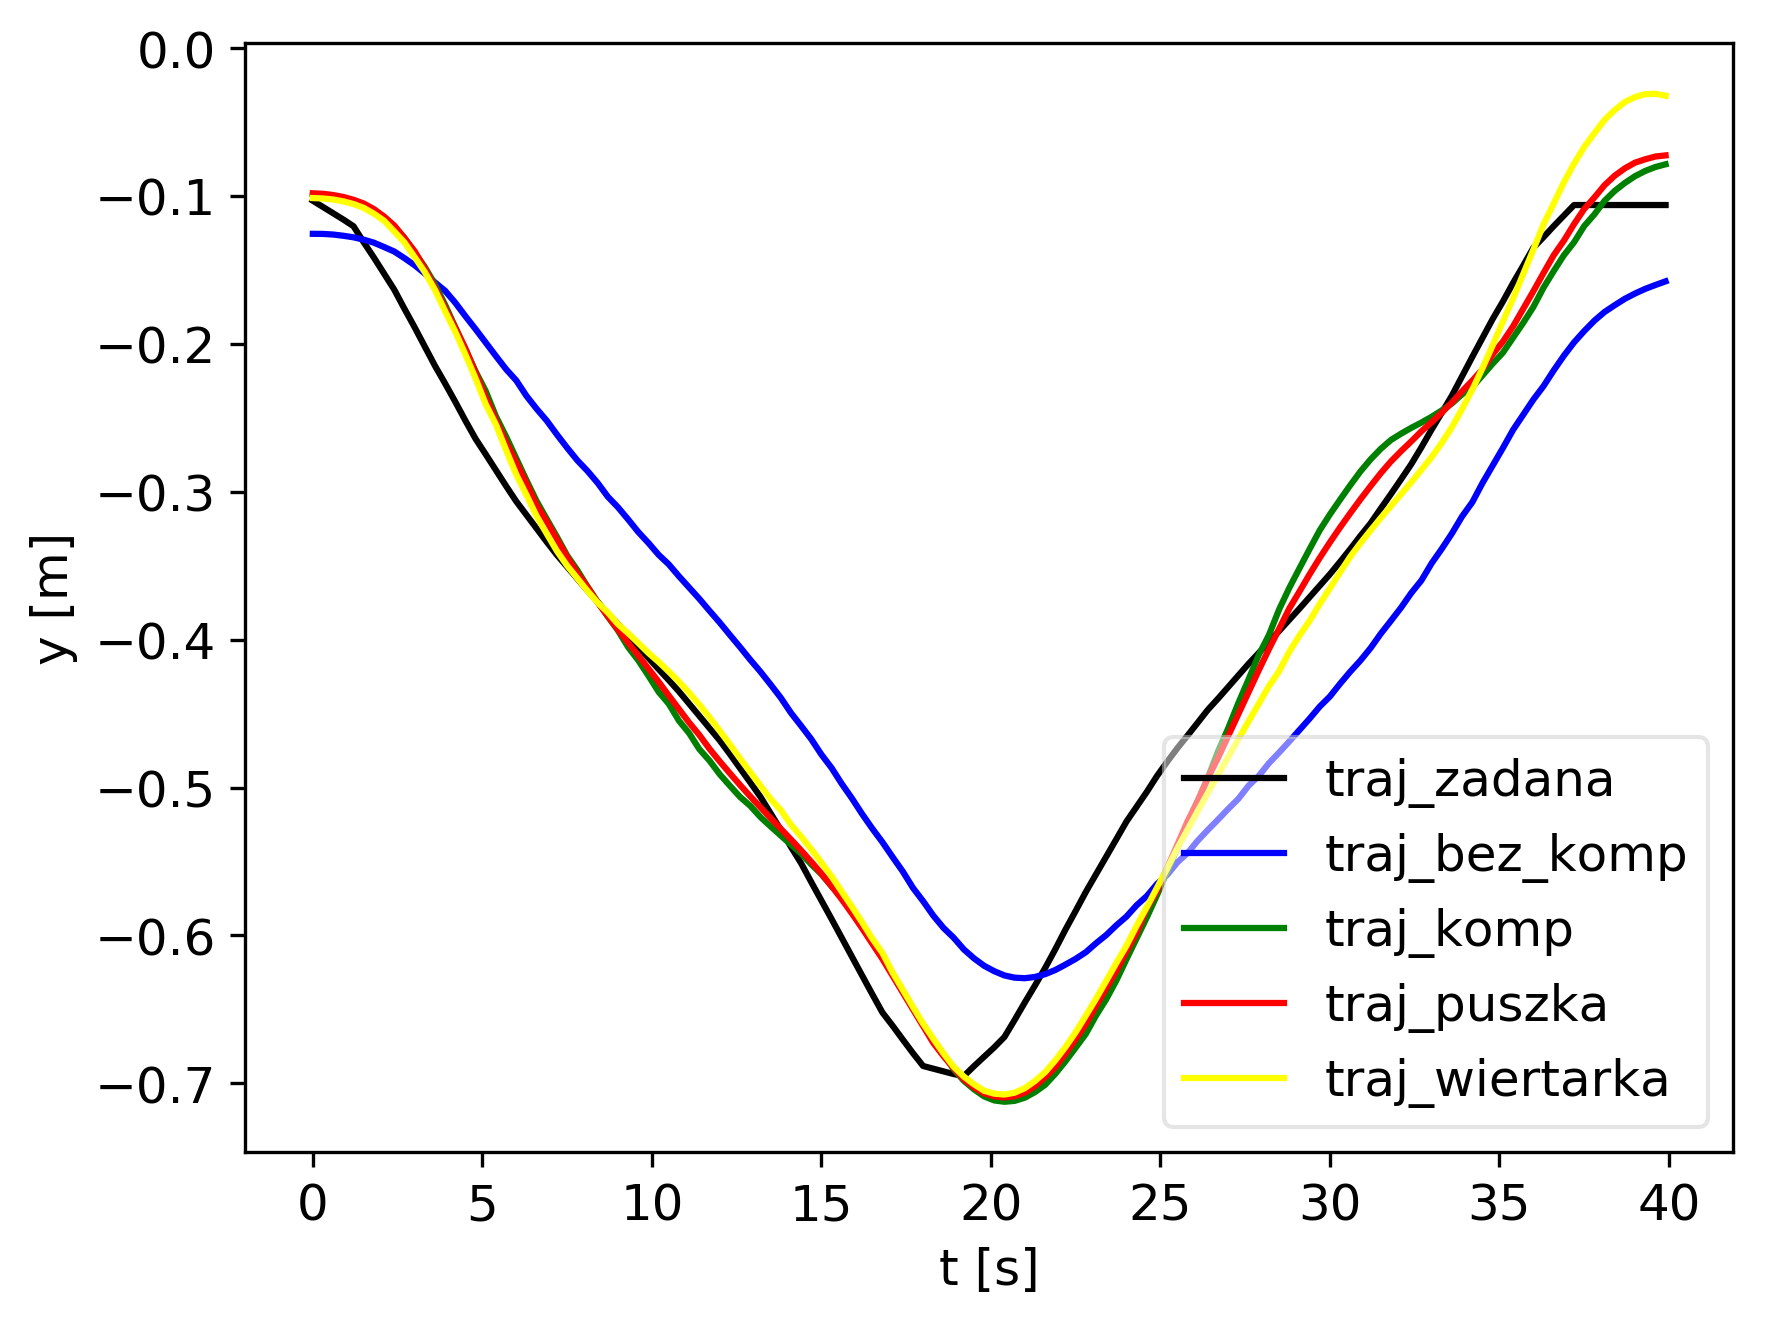
\includegraphics[width=.45\textwidth]{../../velma/przerobione_testy/out/osemka/common_ay.png}
	}
	
	\hfill
	\subfigure[Os $Z$]{
		\label{fig:osemka_az}
		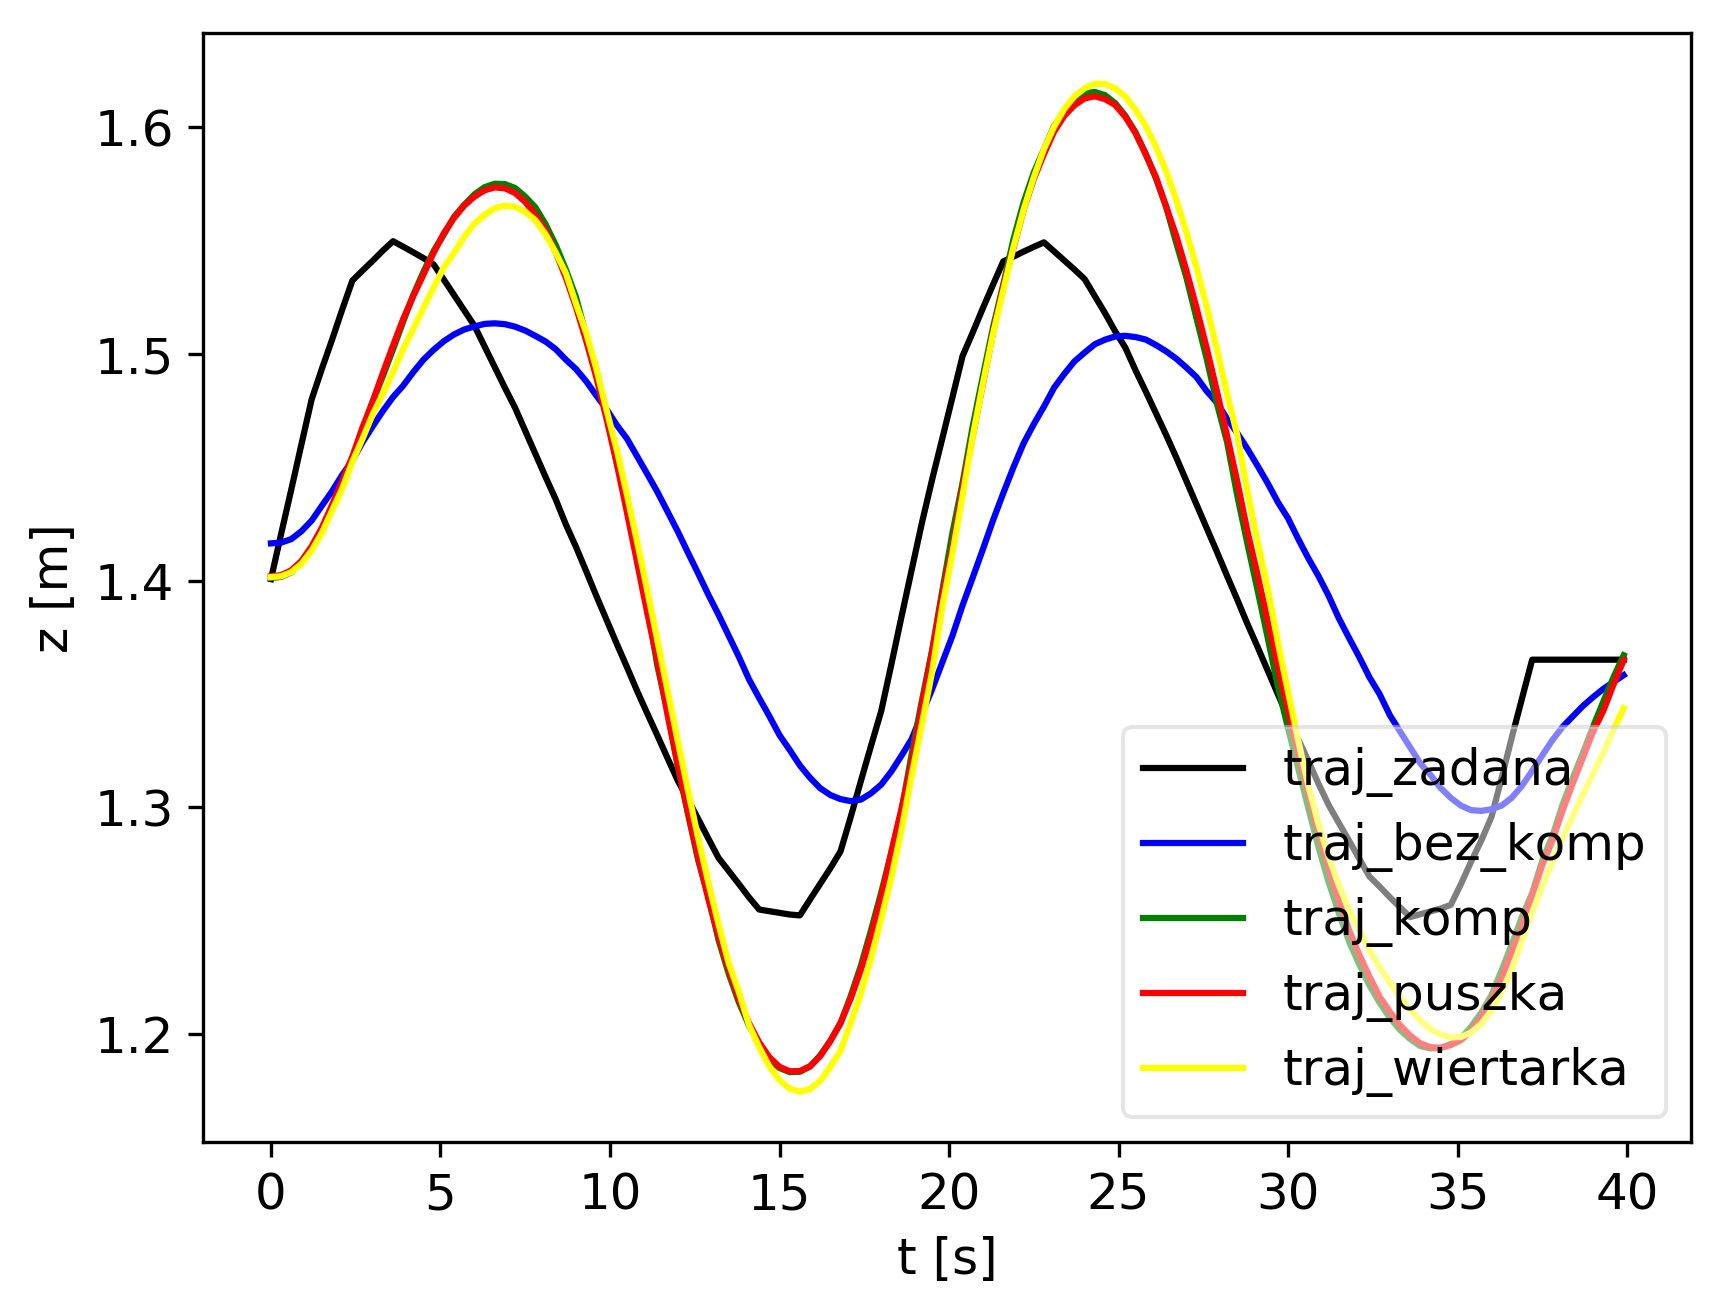
\includegraphics[width=.45\textwidth]{../../velma/przerobione_testy/out/osemka/common_az.png}
	}

	\caption{Ruch osemkowy. Porownanie trajektorii pozycji w zaleznosci od czasu.}
	\label{fig:osemka_a}

\end{figure}


\begin{figure}[h]
	\centering
	\subfigure[Kat osi $X$]{
		\label{fig:osemka_rotx}
		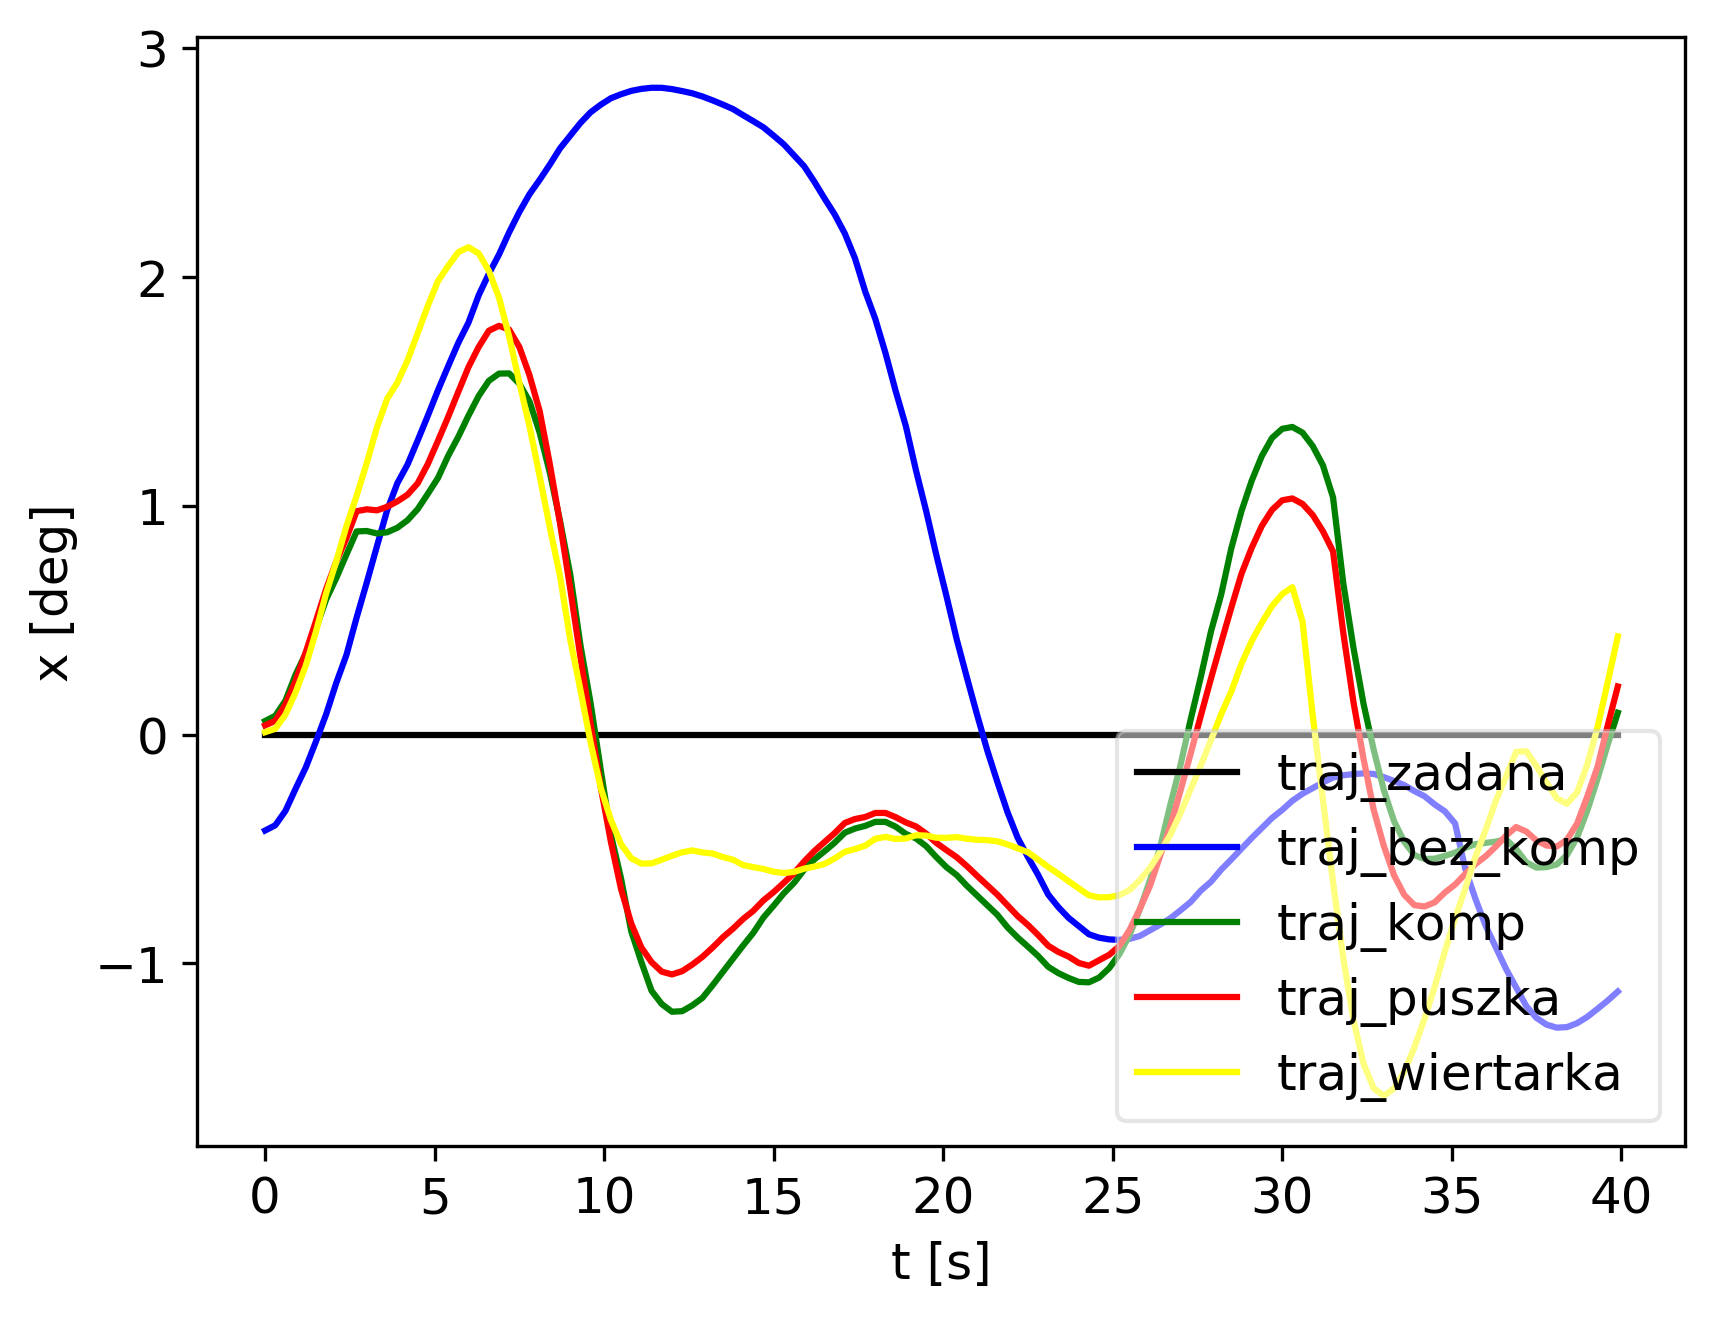
\includegraphics[width=.45\textwidth]{../../velma/przerobione_testy/out/osemka/common_rotx.png}
	}
	\hfill
	\subfigure[Kat osi $Y$]{
		\label{fig:do_gory_roty}
		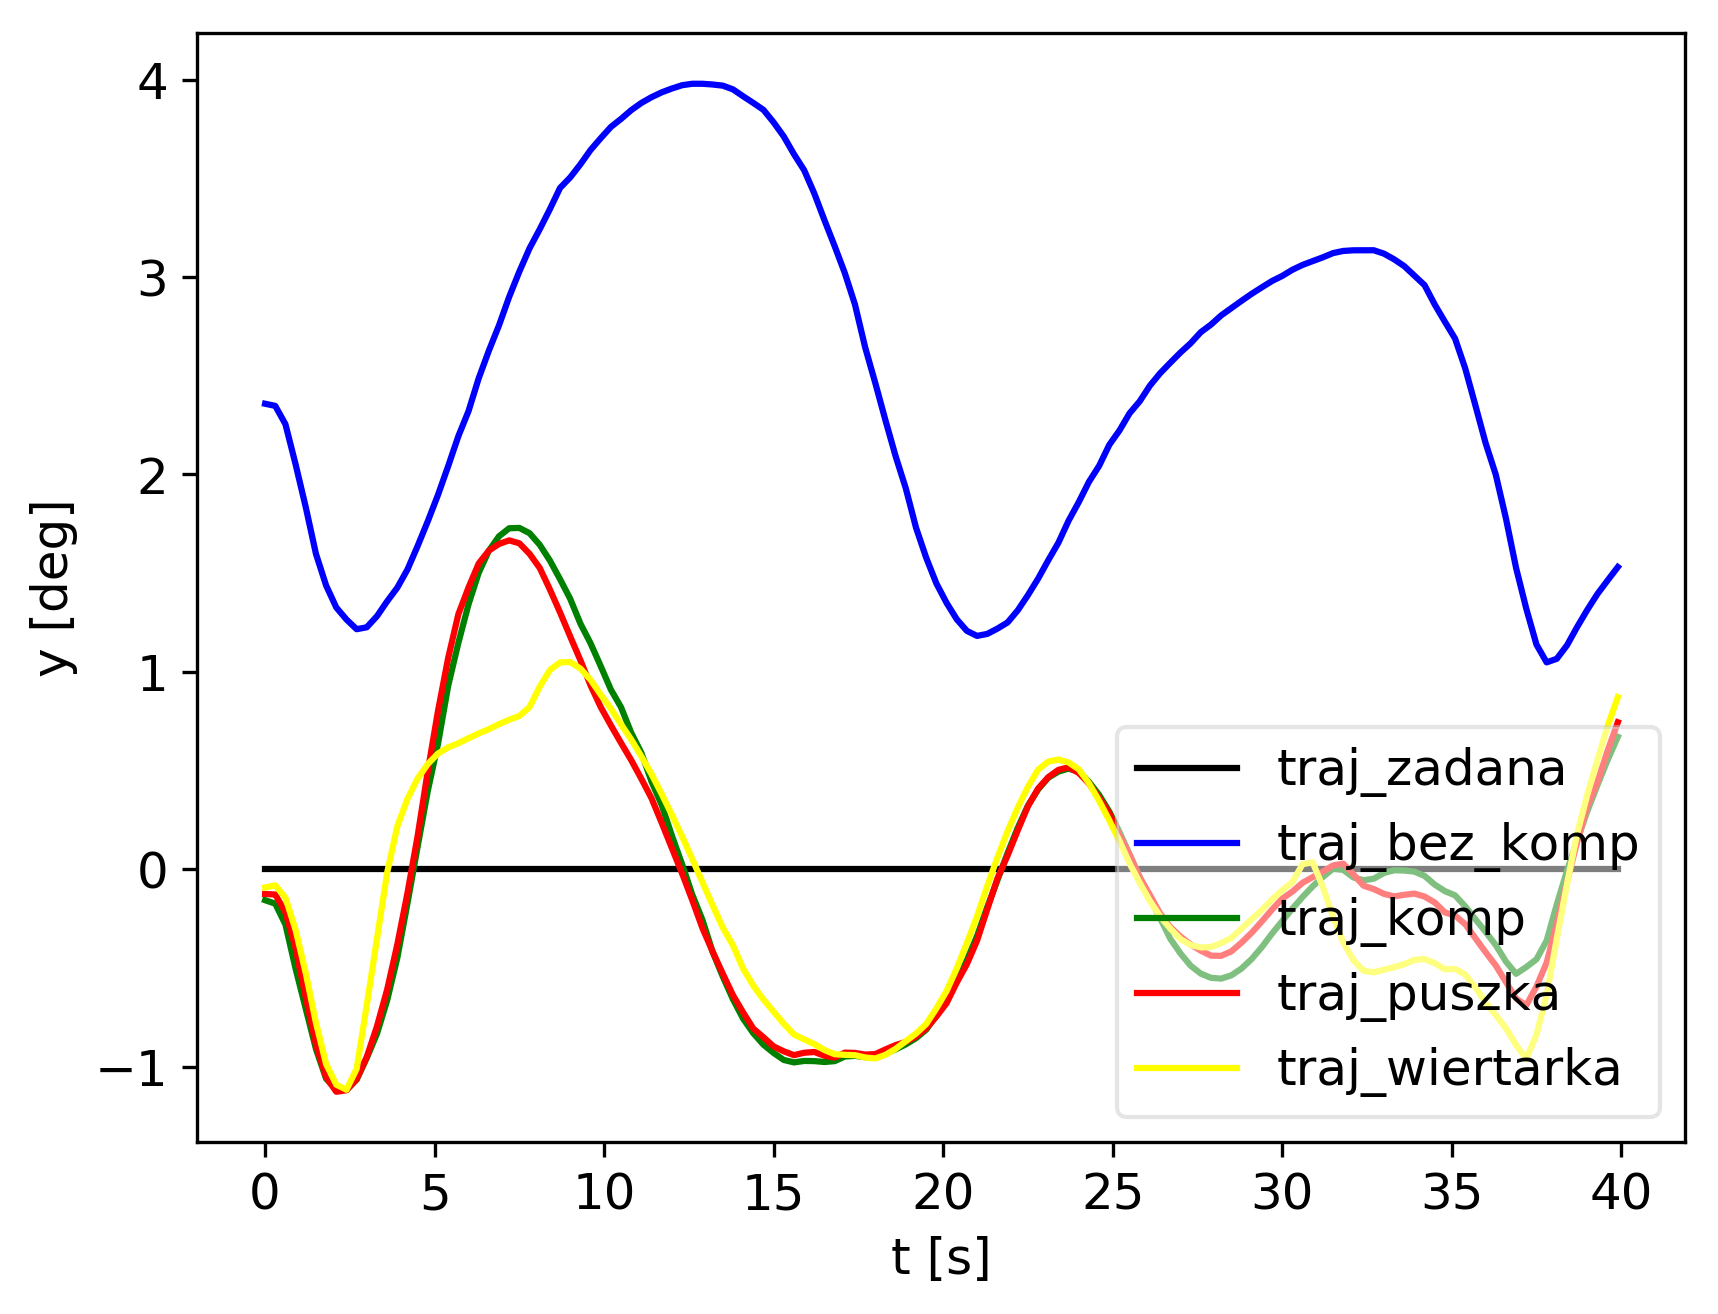
\includegraphics[width=.45\textwidth]{../../velma/przerobione_testy/out/osemka/common_roty.png}
	}
	
	\hfill
	\subfigure[Kat osi $Z$]{
		\label{fig:osemka_rotz}
		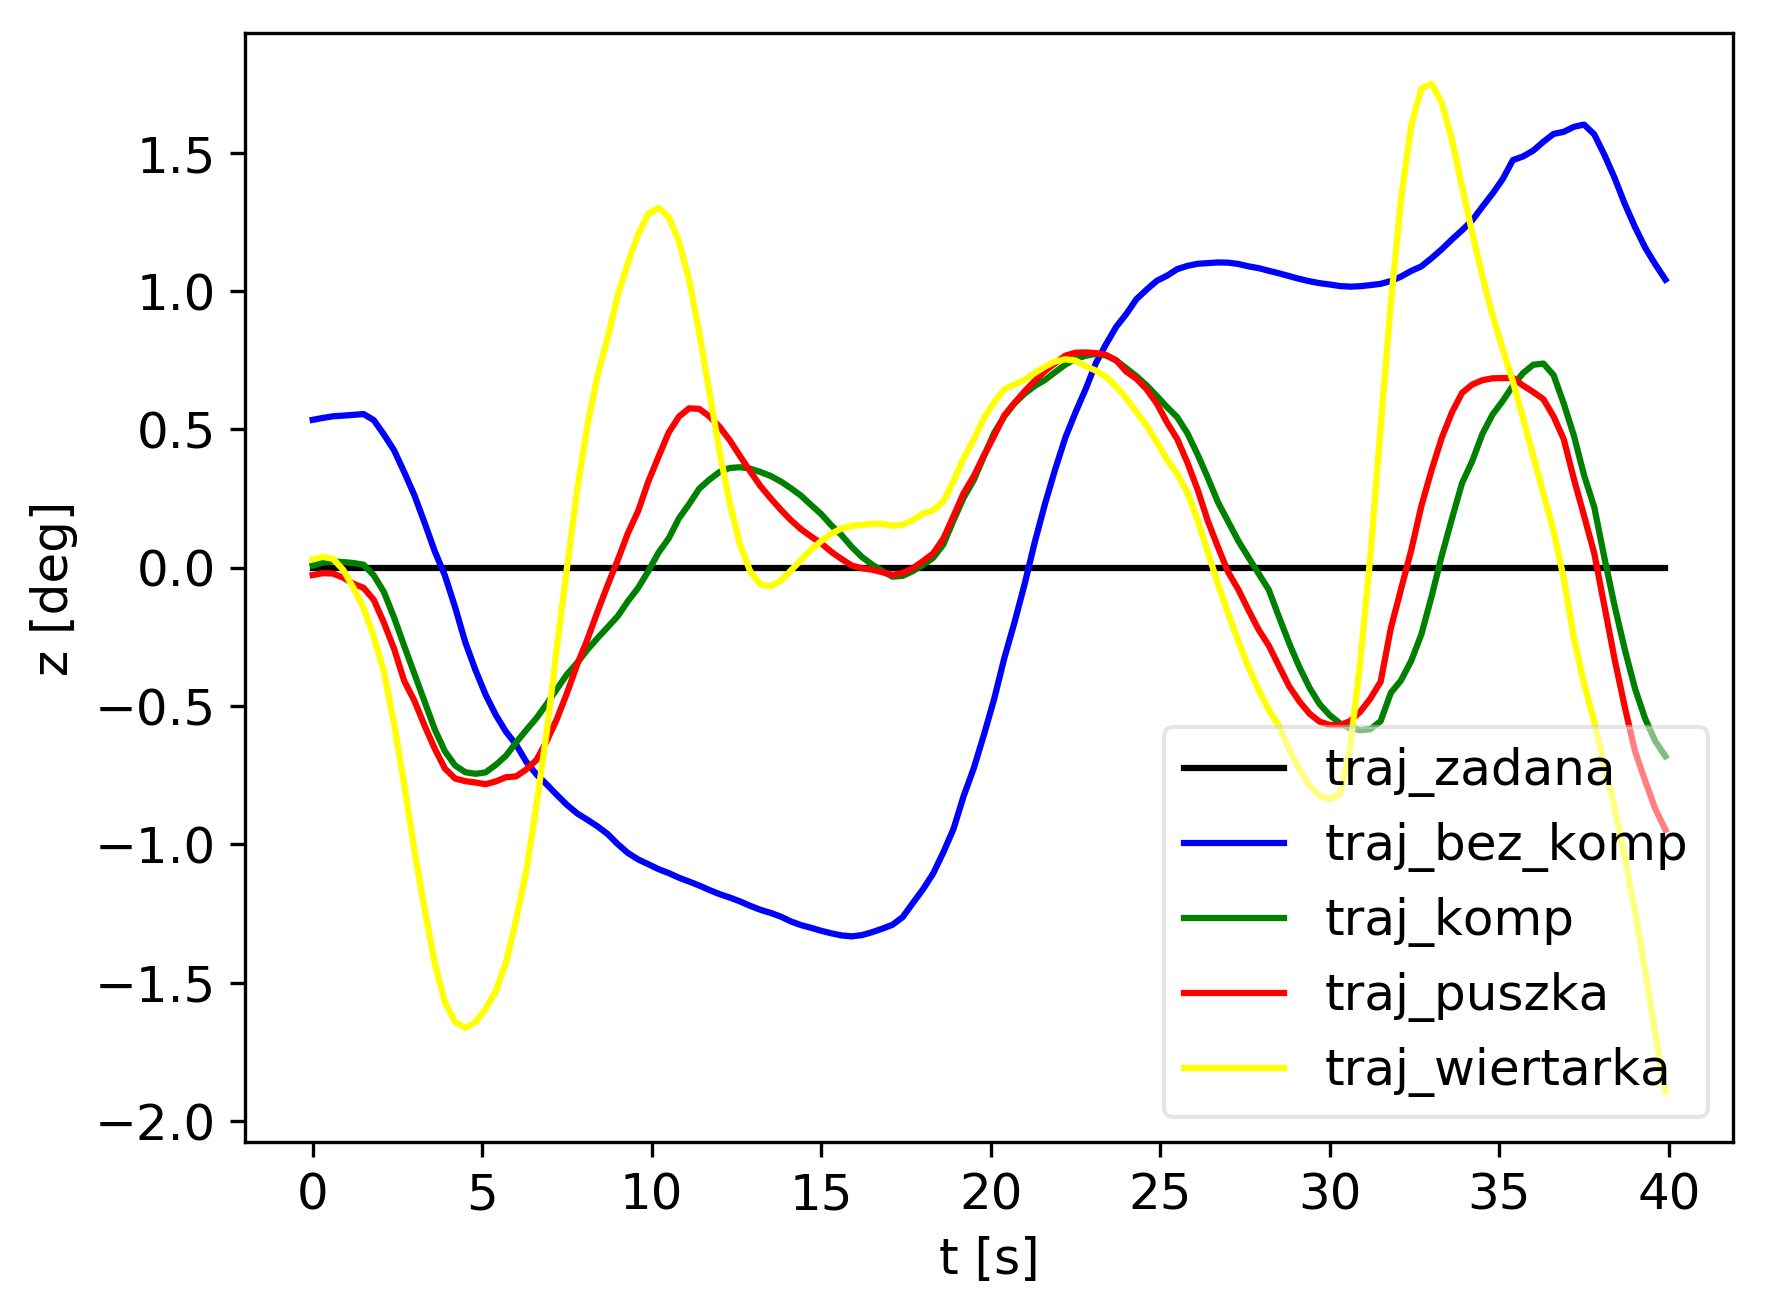
\includegraphics[width=.45\textwidth]{../../velma/przerobione_testy/out/osemka/common_rotz.png}
	}

	\caption{Ruch osemkowy. Porownanie trajektorii katow w notacji Eulera w zaleznosci od czasu.}
	\label{fig:osemka_rot}

\end{figure}

\begin{figure}
	\centering
	\subfigure[Brak algorytmu kompensacji]{
		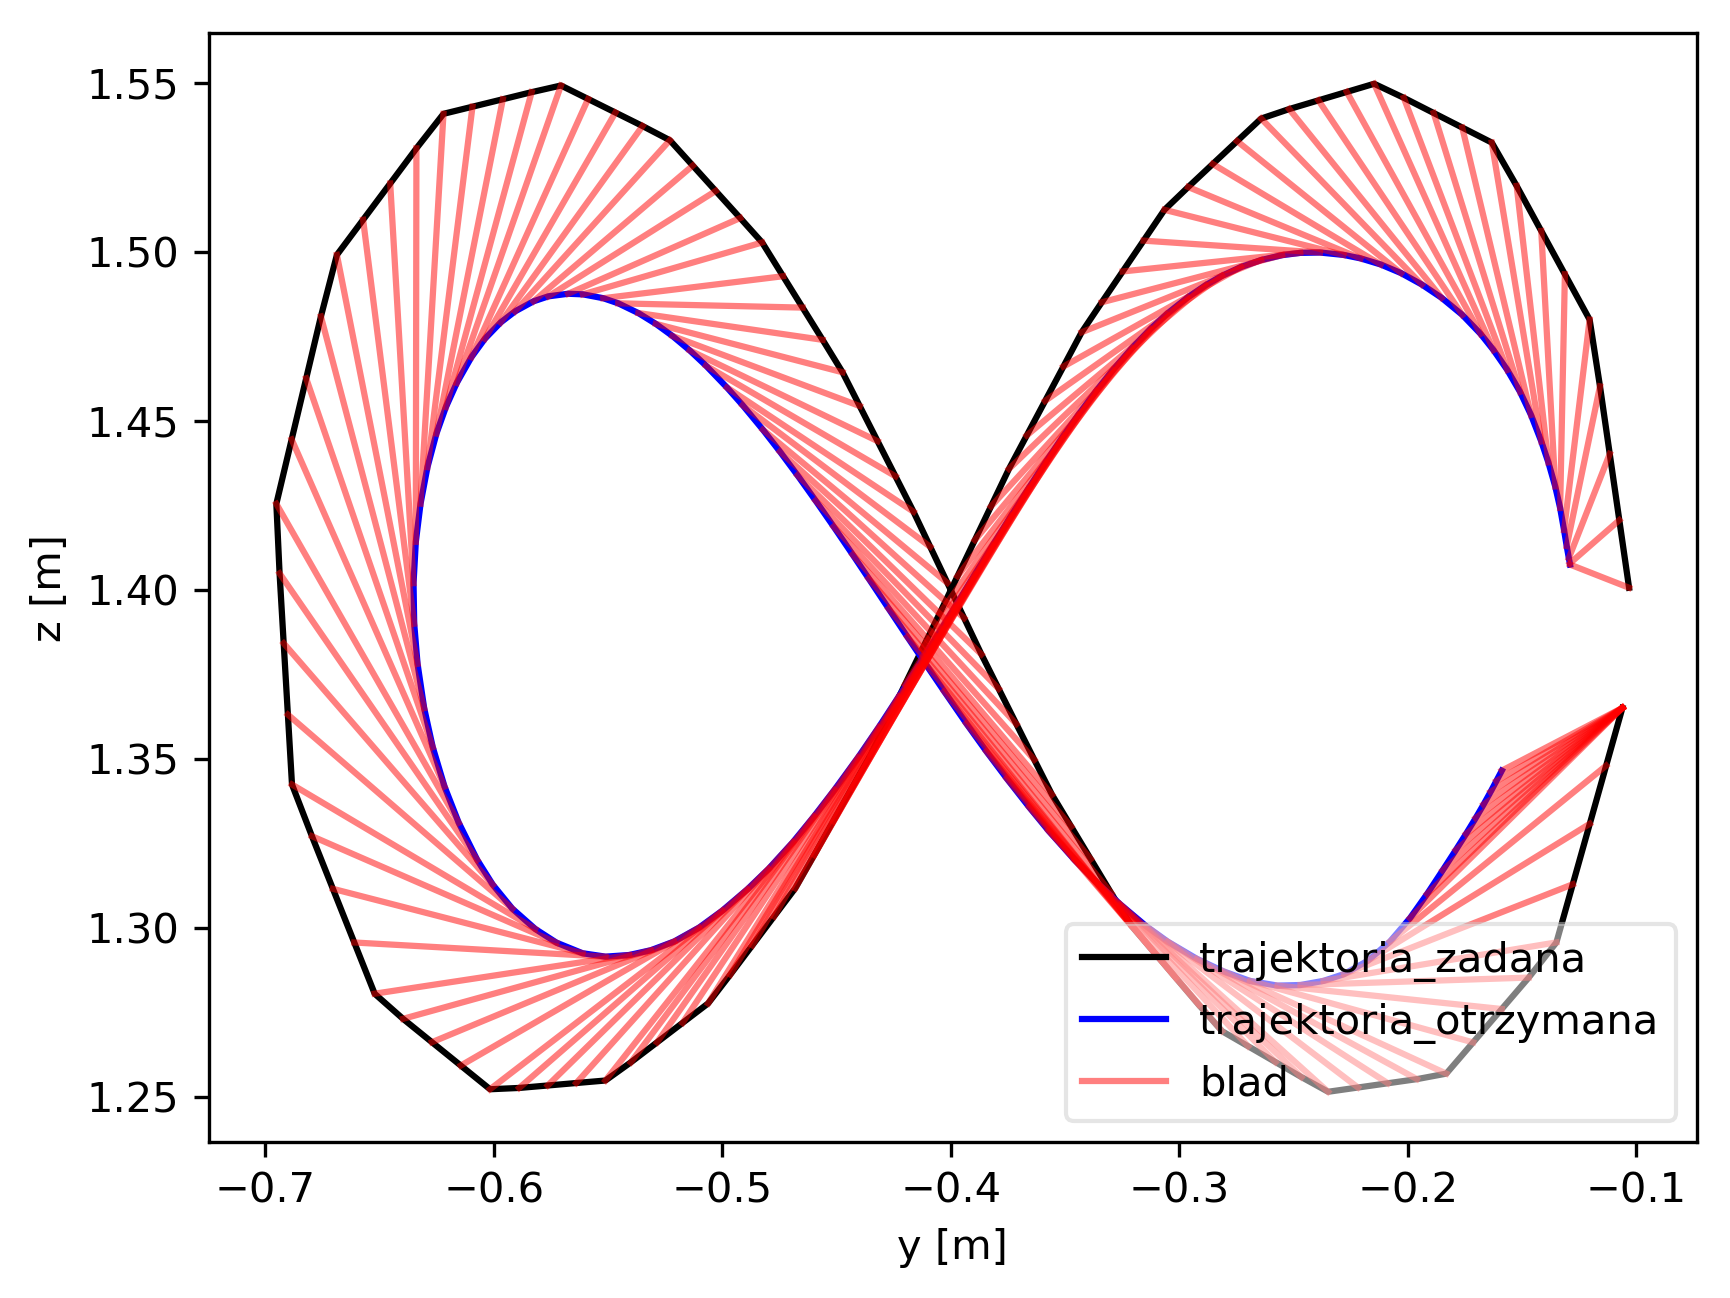
\includegraphics[width=.45\textwidth]{../../velma/przerobione_testy/out/osemka/yz_ate_plot_podnoszenie_miekki_bez_brak.png}
	}
	\hfill
	\subfigure[Zalaczony algorytm kompnesacji]{
		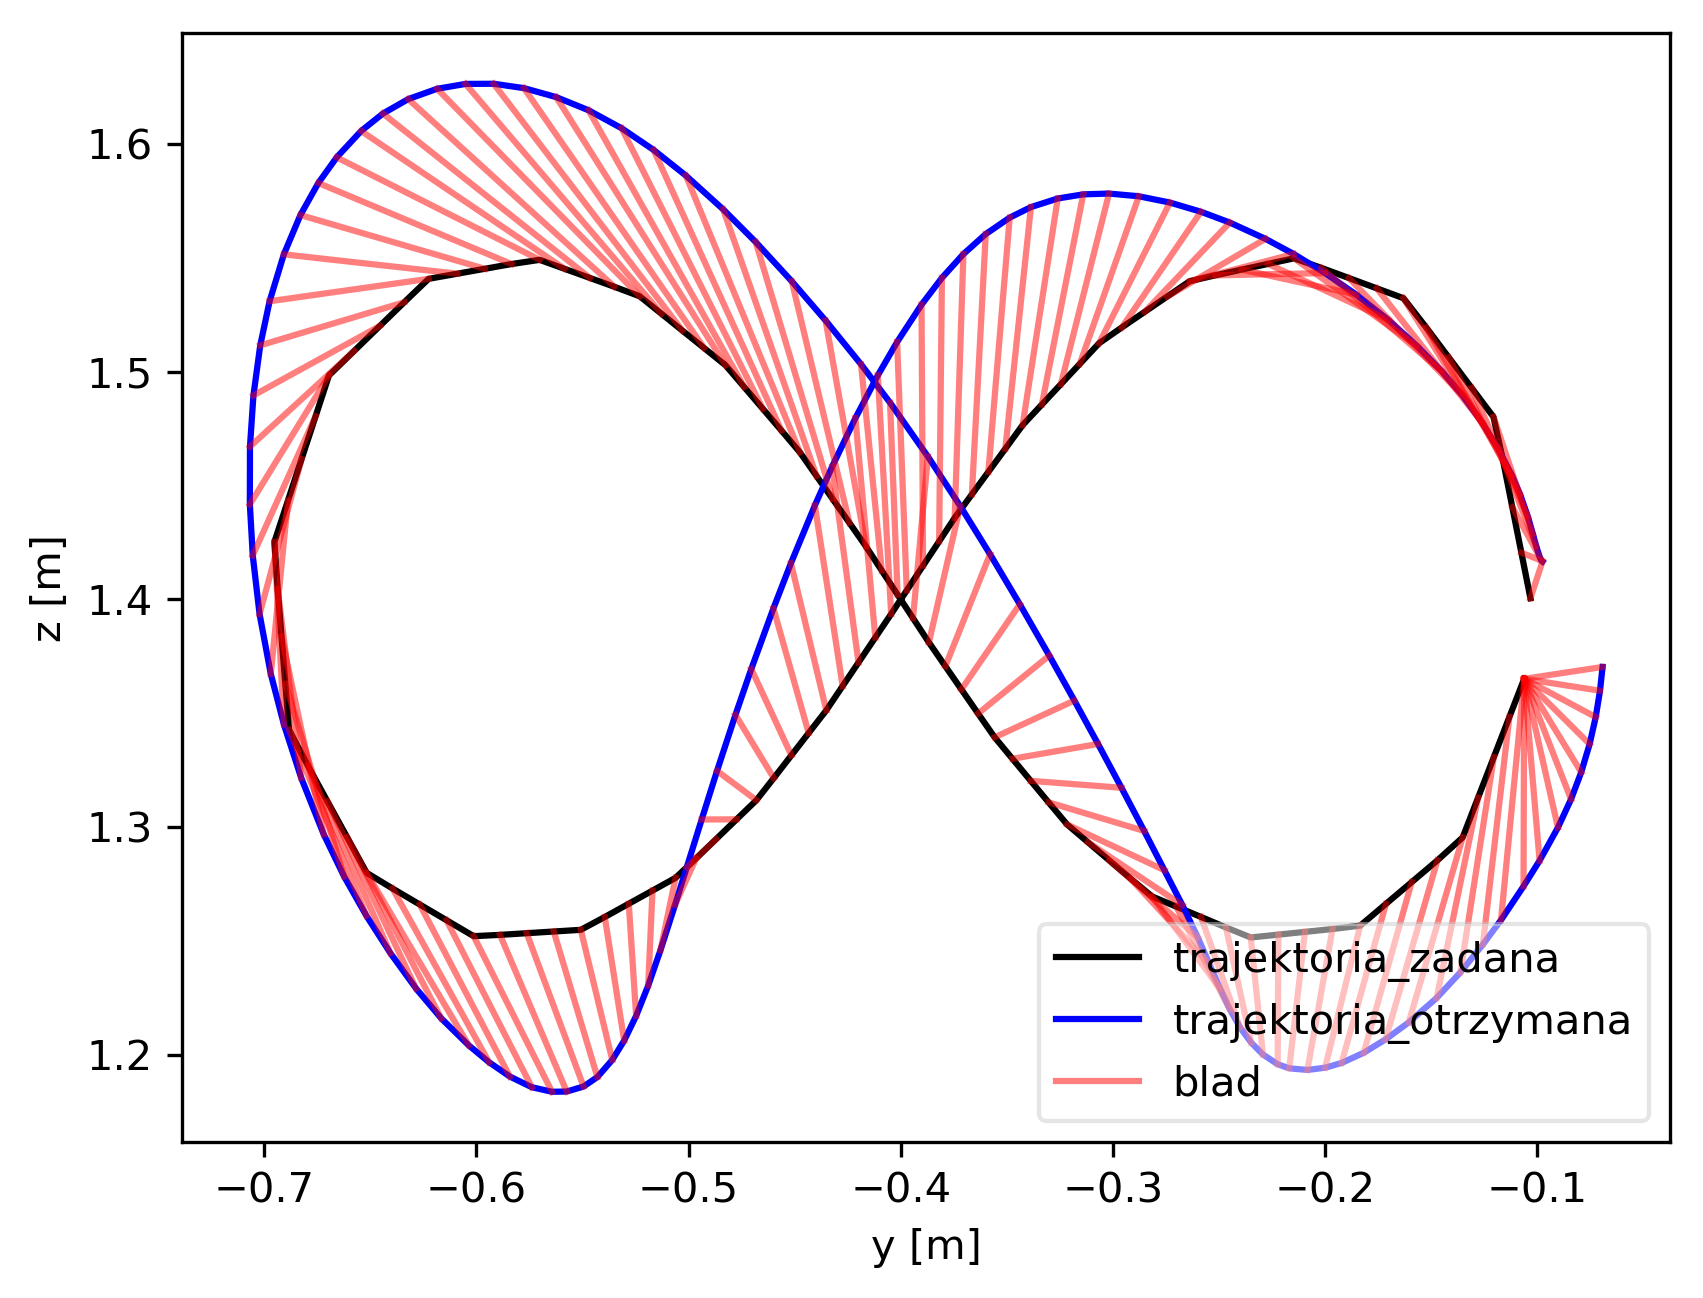
\includegraphics[width=.45\textwidth]{../../velma/przerobione_testy/out/osemka/yz_ate_plot_podnoszenie_miekki_komp_brak.png}
	}
	\caption{Porownanie trajektorii chwytaka w osiach $Y$ i $Z$}
	\label{fig:osemka_porow_komp}
\end{figure}

\begin{figure}
	\centering
	\subfigure[Trajektoria z chwycona puszka]{
		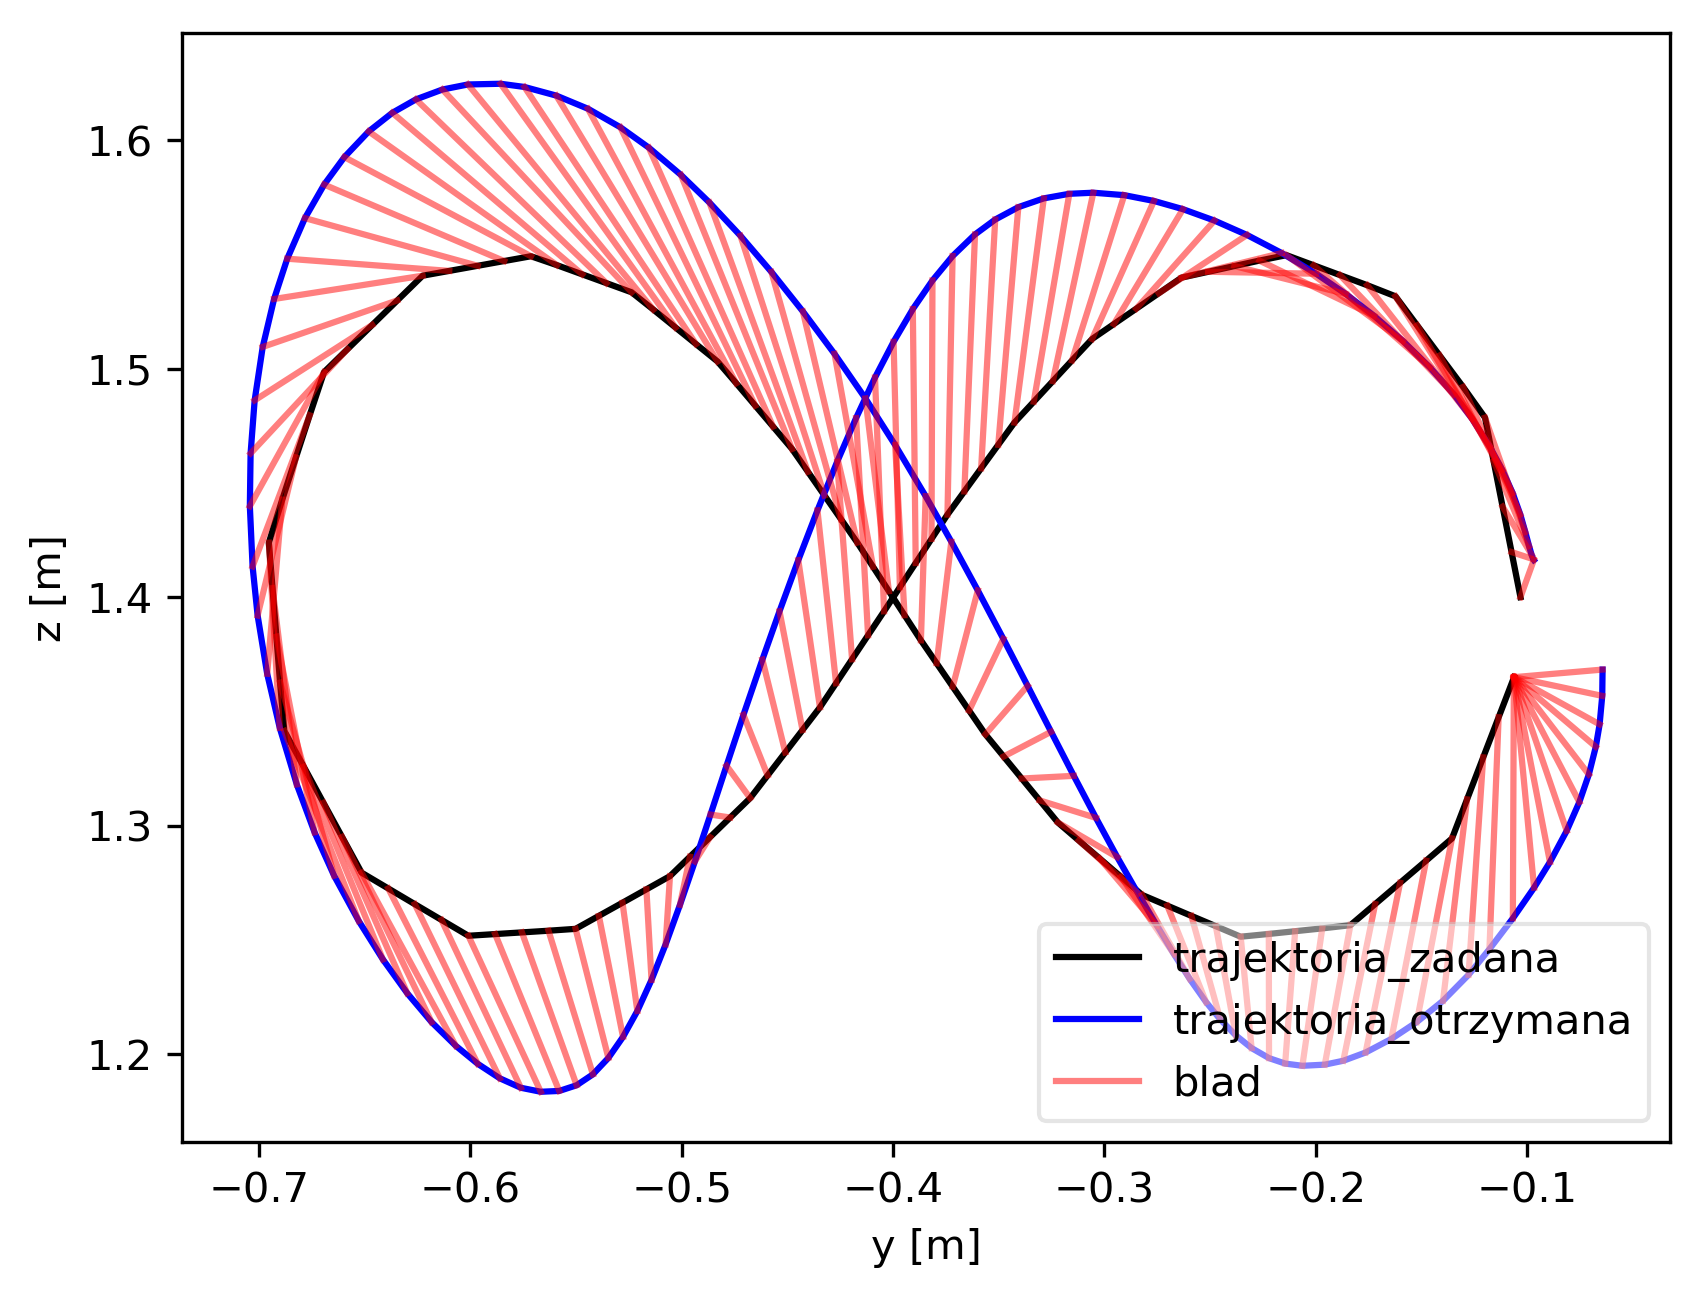
\includegraphics[width=.45\textwidth]{../../velma/przerobione_testy/out/osemka/yz_ate_plot_podnoszenie_miekki_komp_piwo.png}
	}
	\hfill
	\subfigure[Trajektoria z chwycona wiertarka]{
		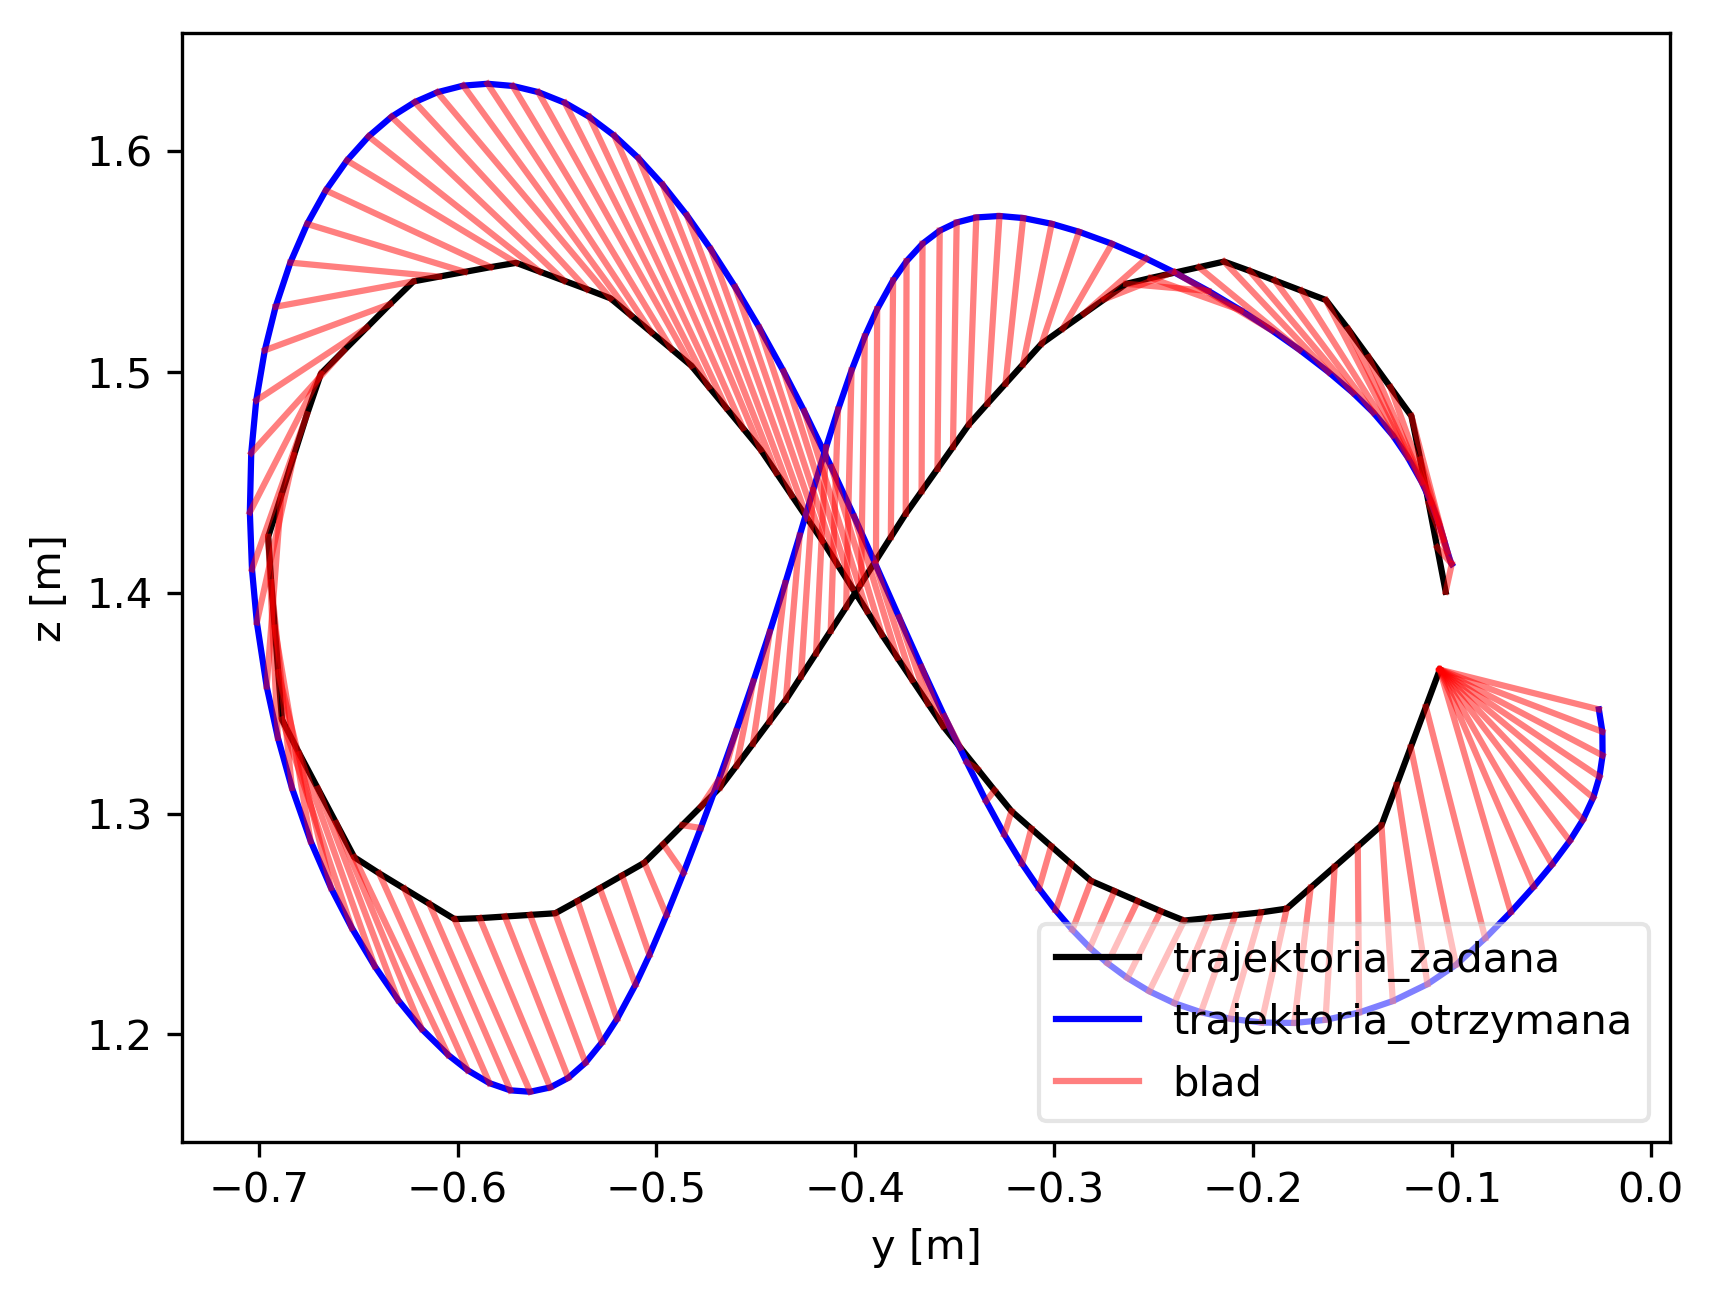
\includegraphics[width=.45\textwidth]{../../velma/przerobione_testy/out/osemka/yz_ate_plot_podnoszenie_miekki_komp_wiertarka.png}
	}
	\caption{Porownanie trajektorii chwytaka w osiach $Y$ i $Z$}
	\label{fig:osemka_porow_przedm}
\end{figure}


\begin{figure}
	\centering
	\subfigure[Brak algorytmu kompensacji]{
		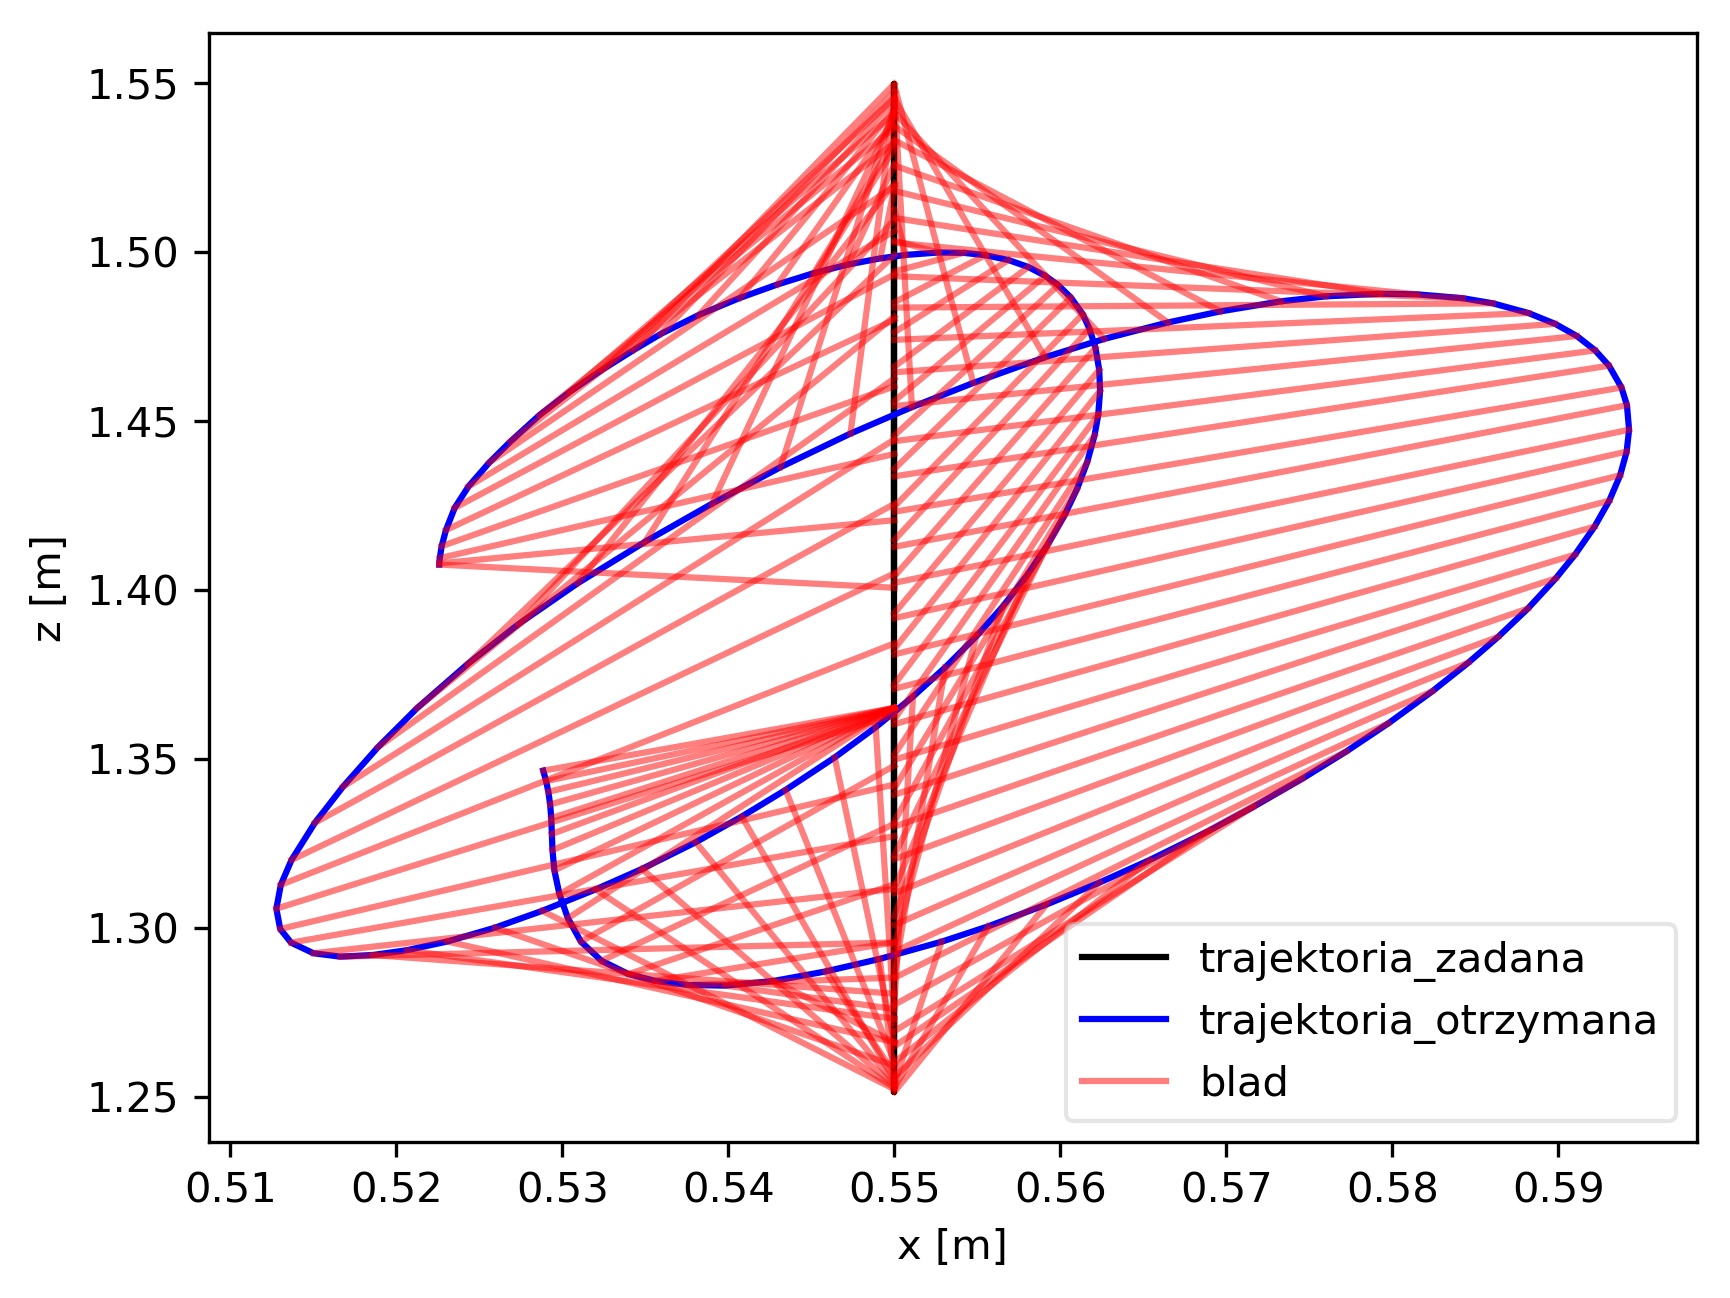
\includegraphics[width=.45\textwidth]{../../velma/przerobione_testy/out/osemka/xz_ate_plot_podnoszenie_miekki_bez_brak.png}
	}
	\hfill
	\subfigure[Zalaczony algorytm kompnesacji]{
		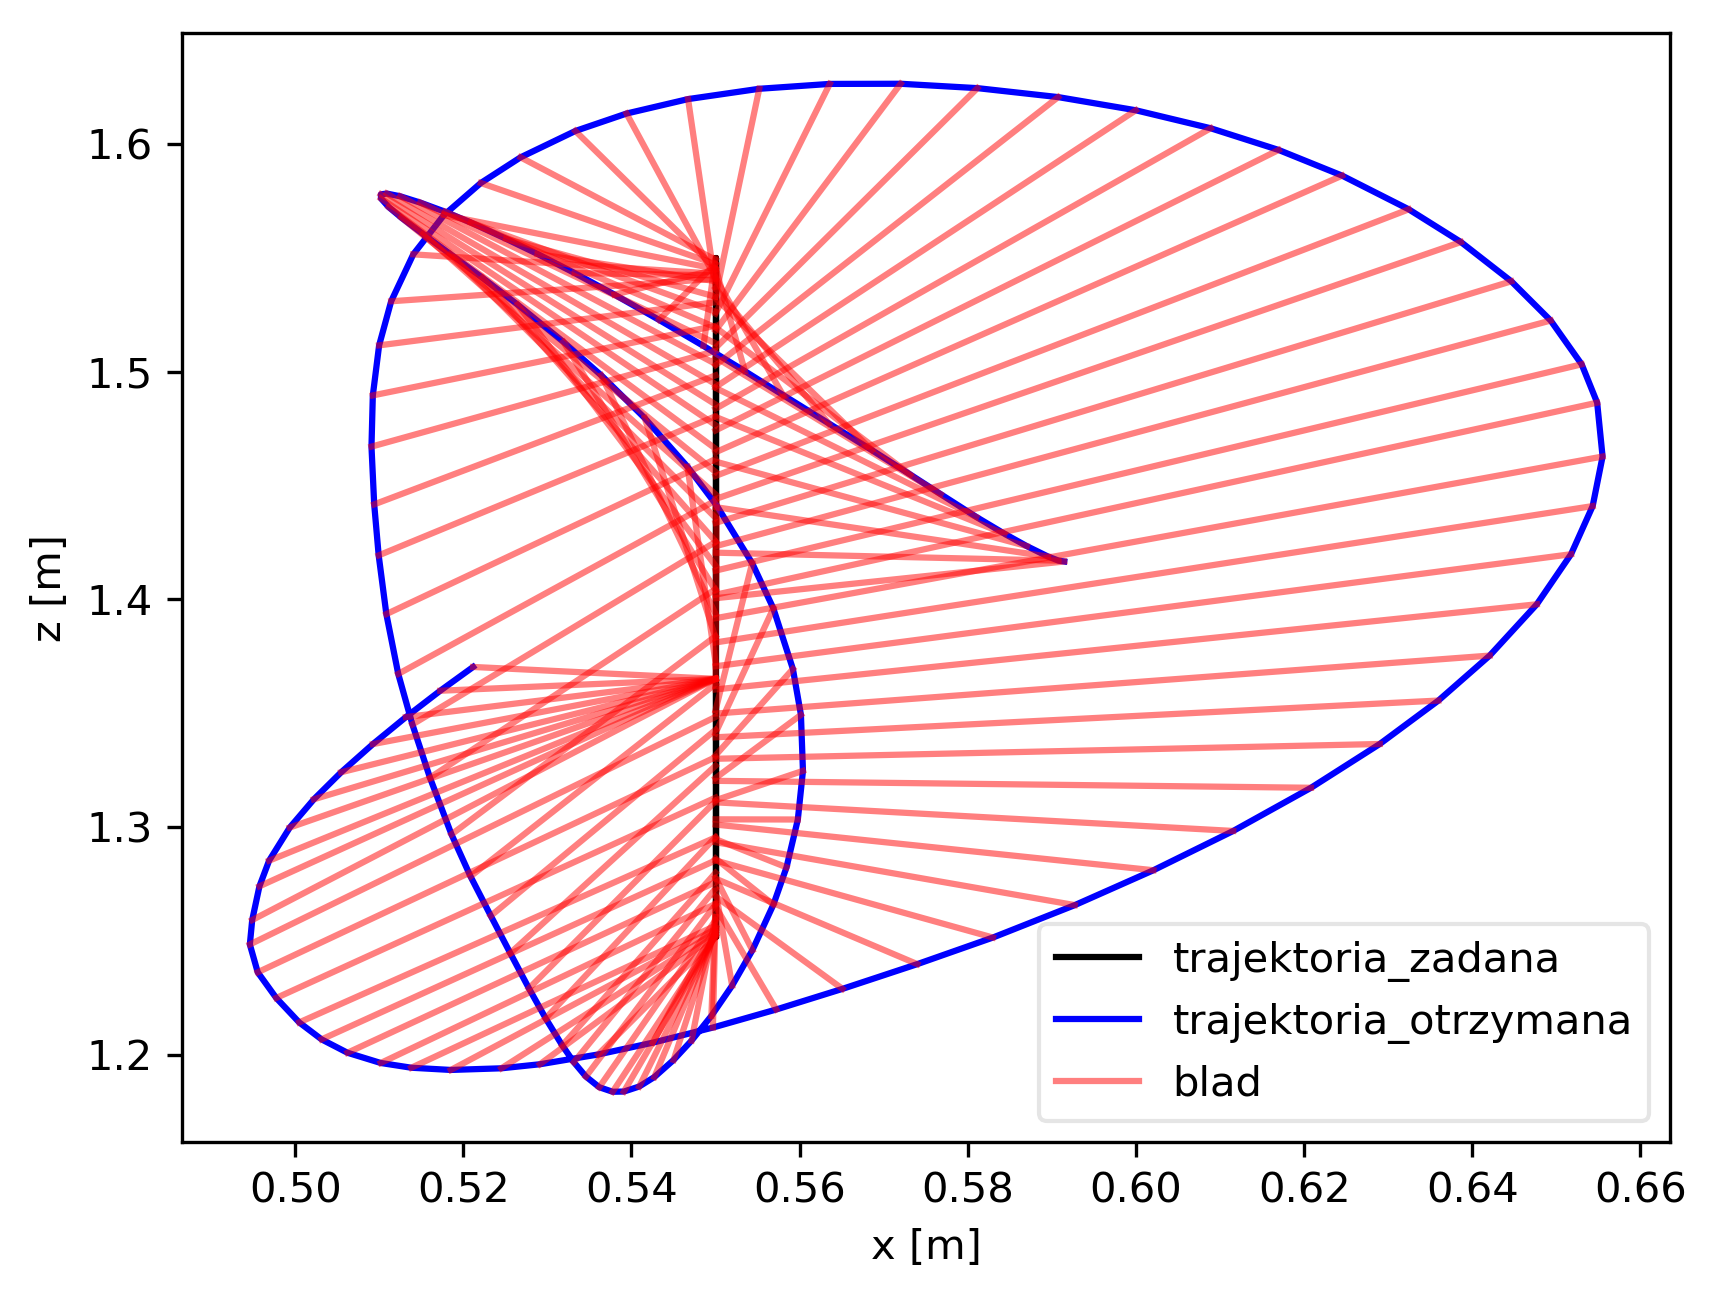
\includegraphics[width=.45\textwidth]{../../velma/przerobione_testy/out/osemka/xz_ate_plot_podnoszenie_miekki_komp_brak.png}
	}
	\caption{Porownanie trajektorii chwytaka w osiach $X$ i $Z$}
	\label{fig:osemka_porow_komp_bok}
\end{figure}

\begin{figure}
	\centering
	\subfigure[Trajektoria z chwycona puszka]{
		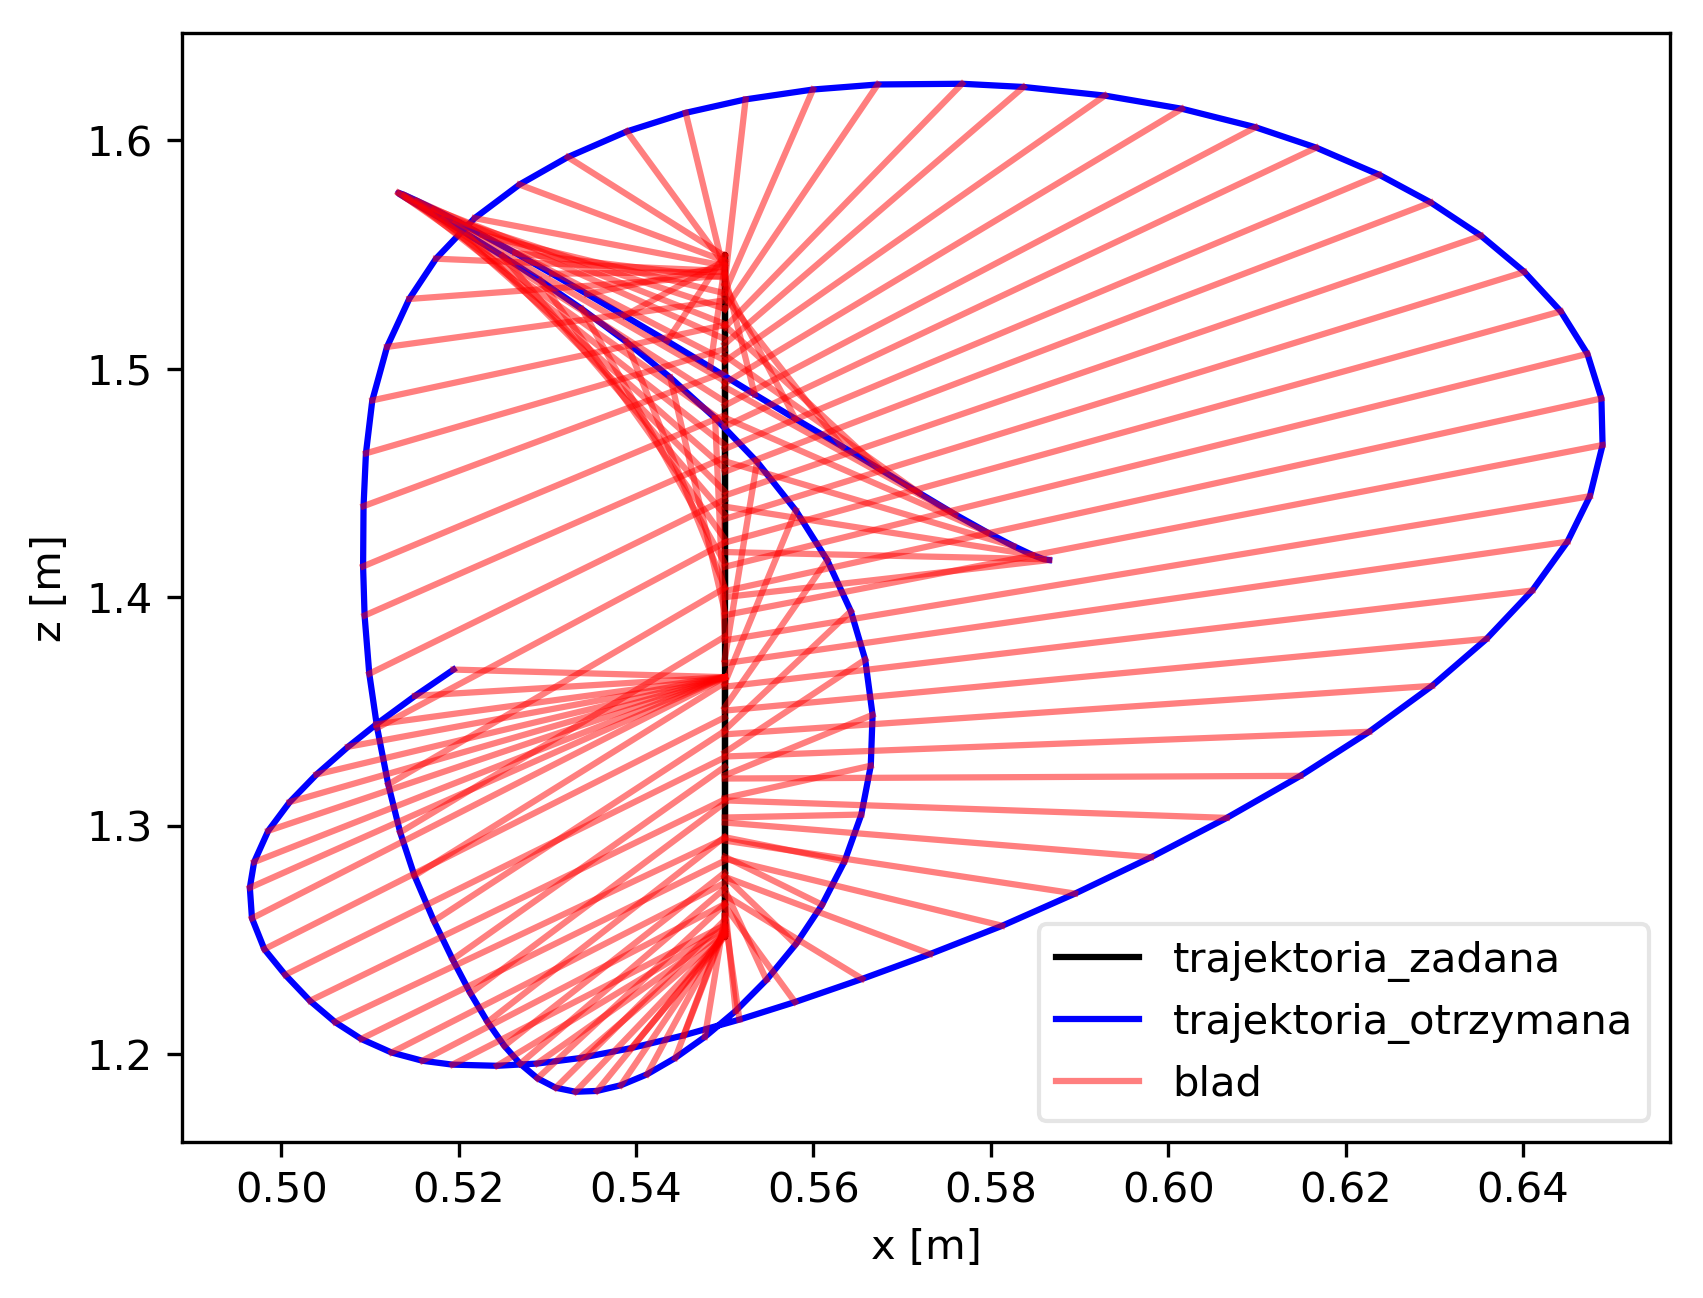
\includegraphics[width=.45\textwidth]{../../velma/przerobione_testy/out/osemka/xz_ate_plot_podnoszenie_miekki_komp_piwo.png}
	}
	\hfill
	\subfigure[Trajektoria z chwycona wiertarka]{
		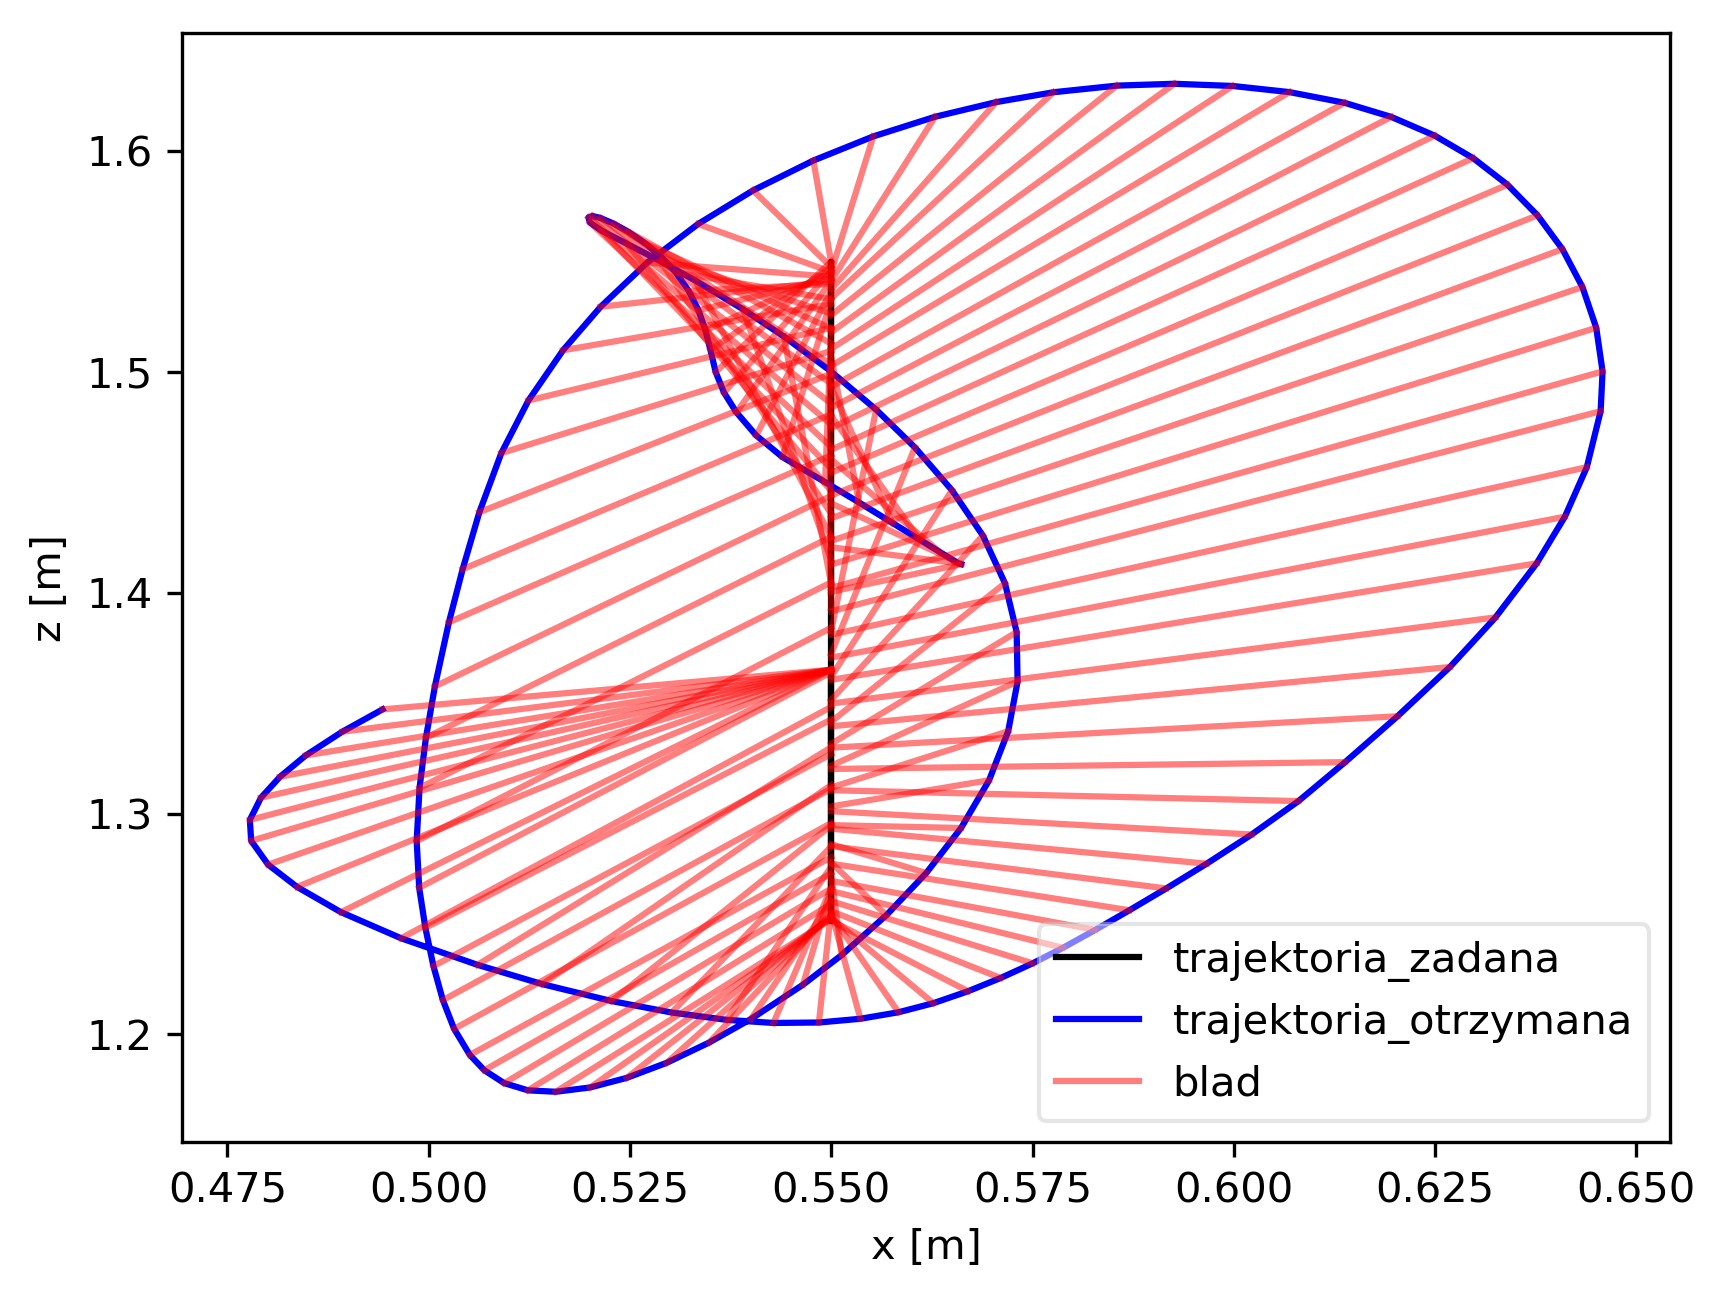
\includegraphics[width=.45\textwidth]{../../velma/przerobione_testy/out/osemka/xz_ate_plot_podnoszenie_miekki_komp_wiertarka.png}
	}
	\caption{Porownanie trajektorii chwytaka w osiach $X$ i $Z$}
	\label{fig:osemka_porow_przedm_bok}
\end{figure}

\begin{figure}
	\centering
	\subfigure[Rzut na wprost]{
		\label{fig:osemka_porow_zbiorcze_a}
		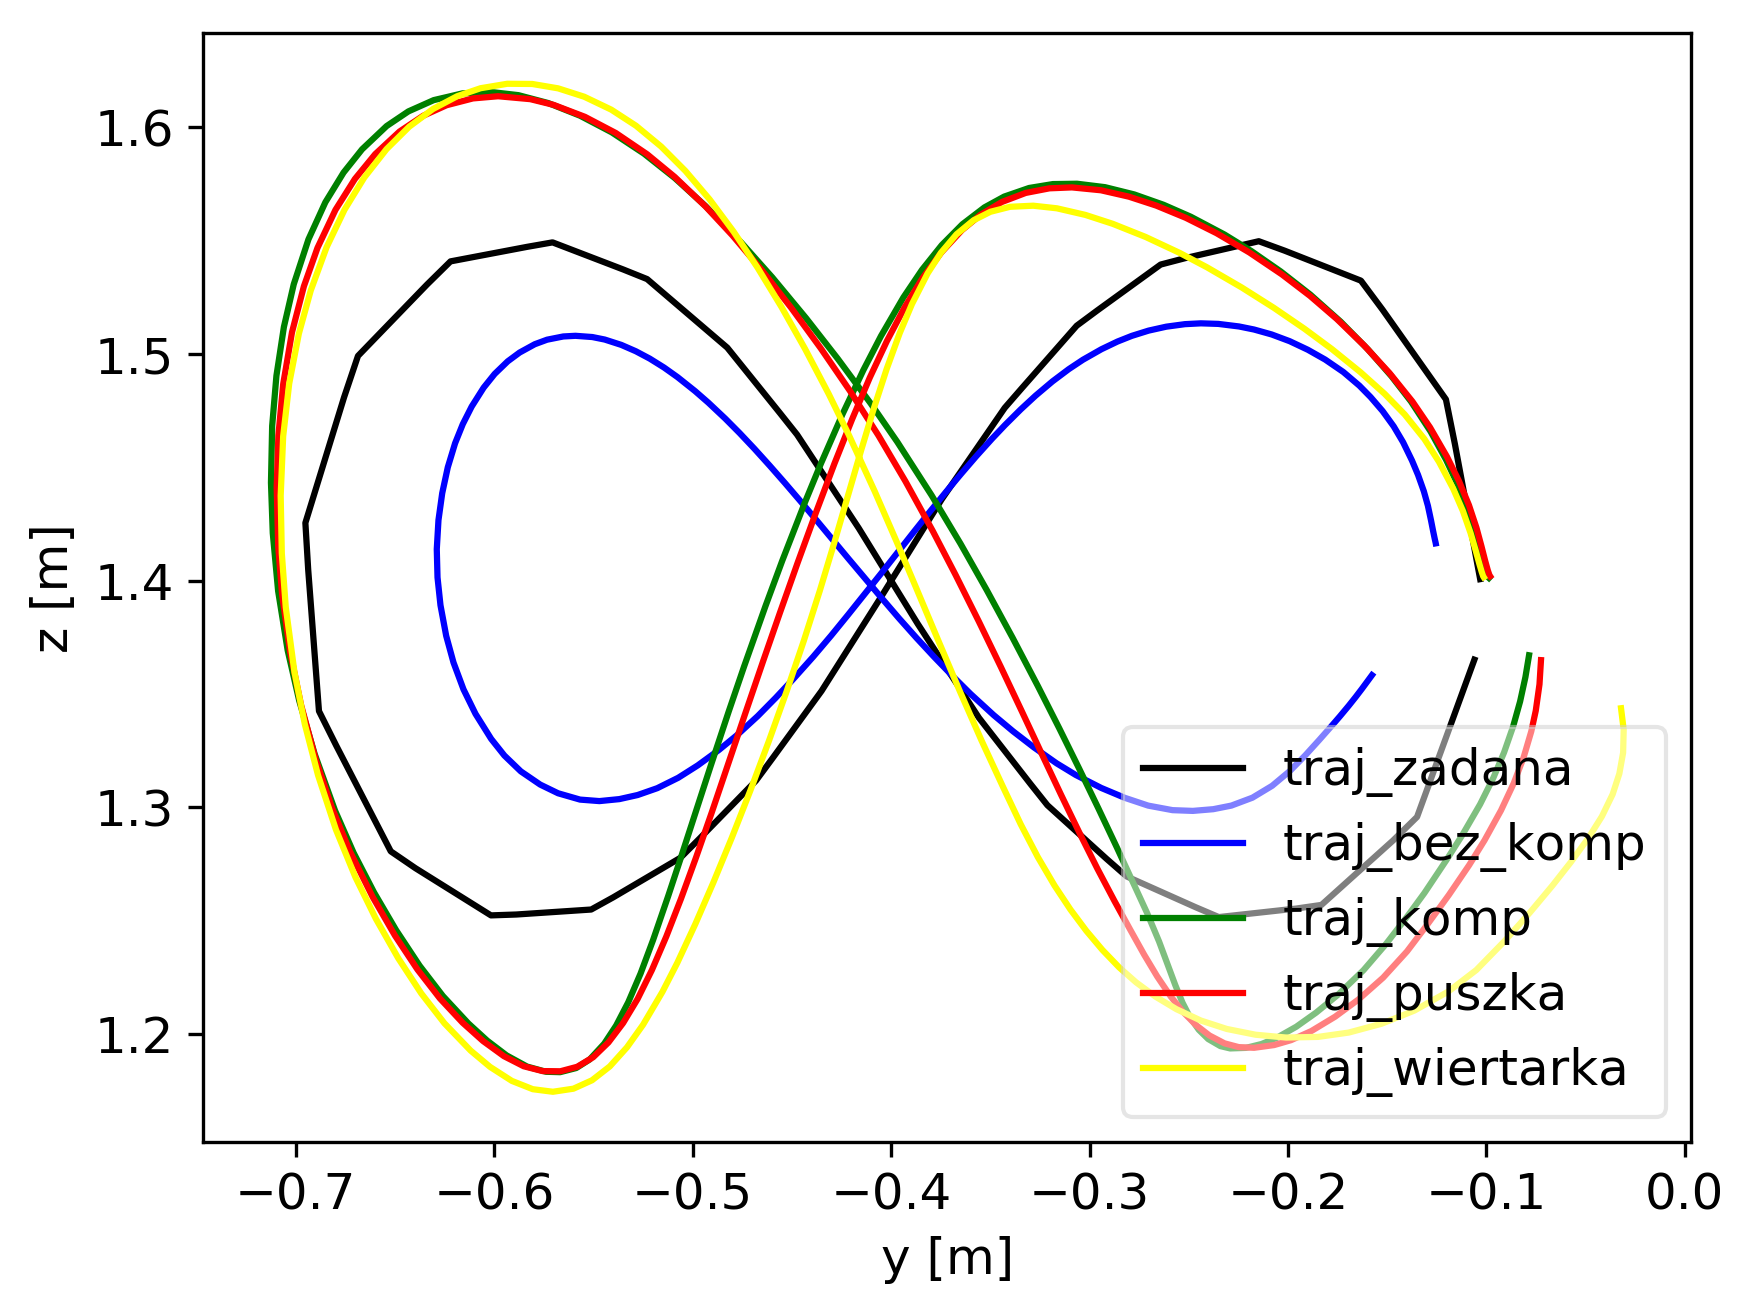
\includegraphics[width=.45\textwidth]{../../velma/przerobione_testy/out/osemka/common_yz.png}
	}
	\hfill
	\subfigure[Rzut z boku]{
		\label{fig:osemka_porow_zbiorcze_b}
		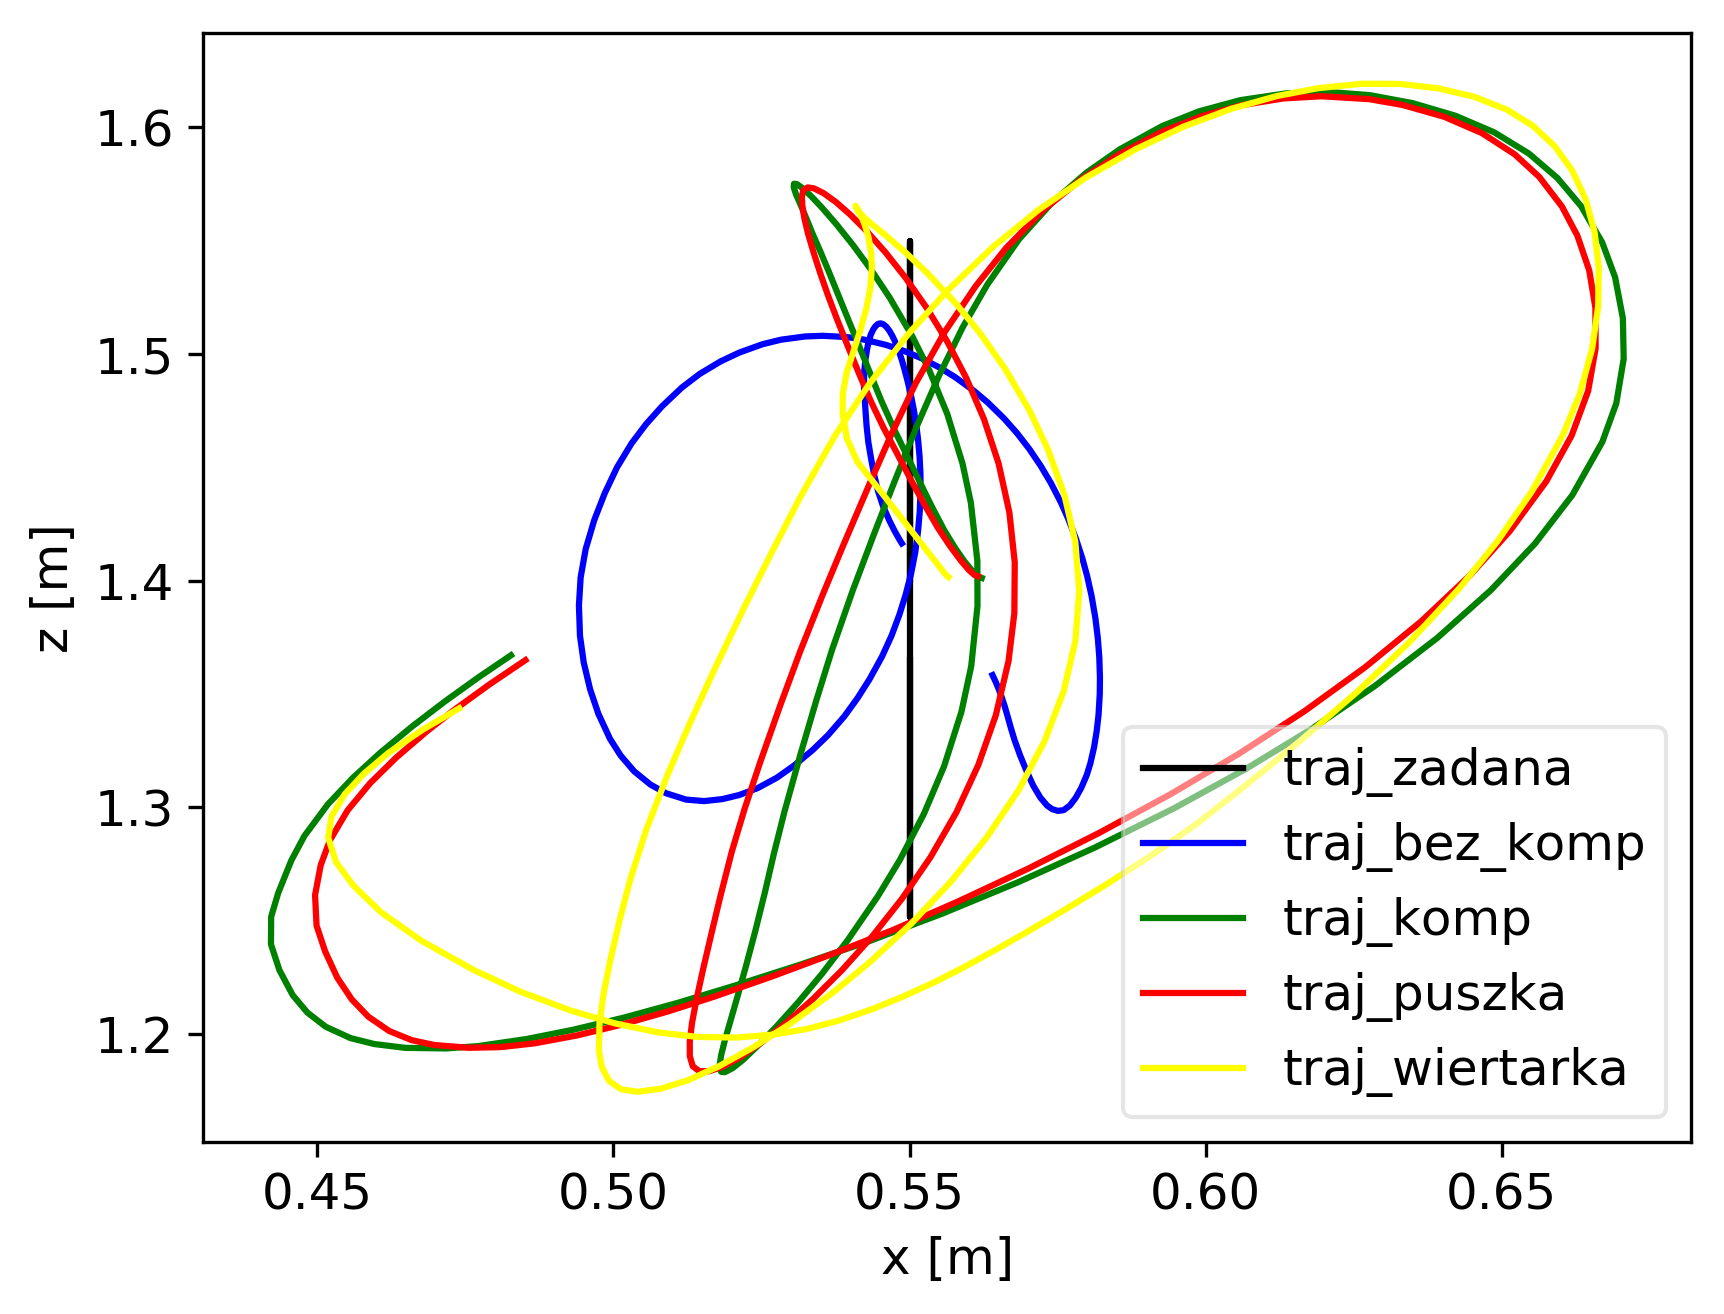
\includegraphics[width=.45\textwidth]{../../velma/przerobione_testy/out/osemka/common_xz.png}
	}
	\caption{Porowanie wszystkich trajektorii bez zaznaczonego bledu.}
	\label{fig:osemka_porow_zbiorcze}
\end{figure}

\subsection{Ruch w bok}

Eksperyment ma przetestowac zachowanie algorytmu kompensacji przy ruchu koncowki w bok. Trajektoria ruchu w rzucie na wprost ruchu zostala zaprezentowana na rys. \ref{fig:w_bok_miekki_porow_komp}, \ref{fig:w_bok_miekki_porow_przedm} i \ref{fig:w_bok_miekki_porow_zbiorcze_a}. 
% Trajektoria widoczna z boku (w osiach $X$ oraz $Z$) zostala zaprezentowana na rys. \ref{fig:w_bok_miekki_porow_komp_bok}, \ref{fig:w_bok_miekki_porow_przedm_bok} i \ref{fig:w_bok_miekki_porow_zbiorcze_b}.
\begin{figure}[h]
	\centering
	\subfigure[Os $X$]{
		\label{fig:w_bok_miekki_ax}
		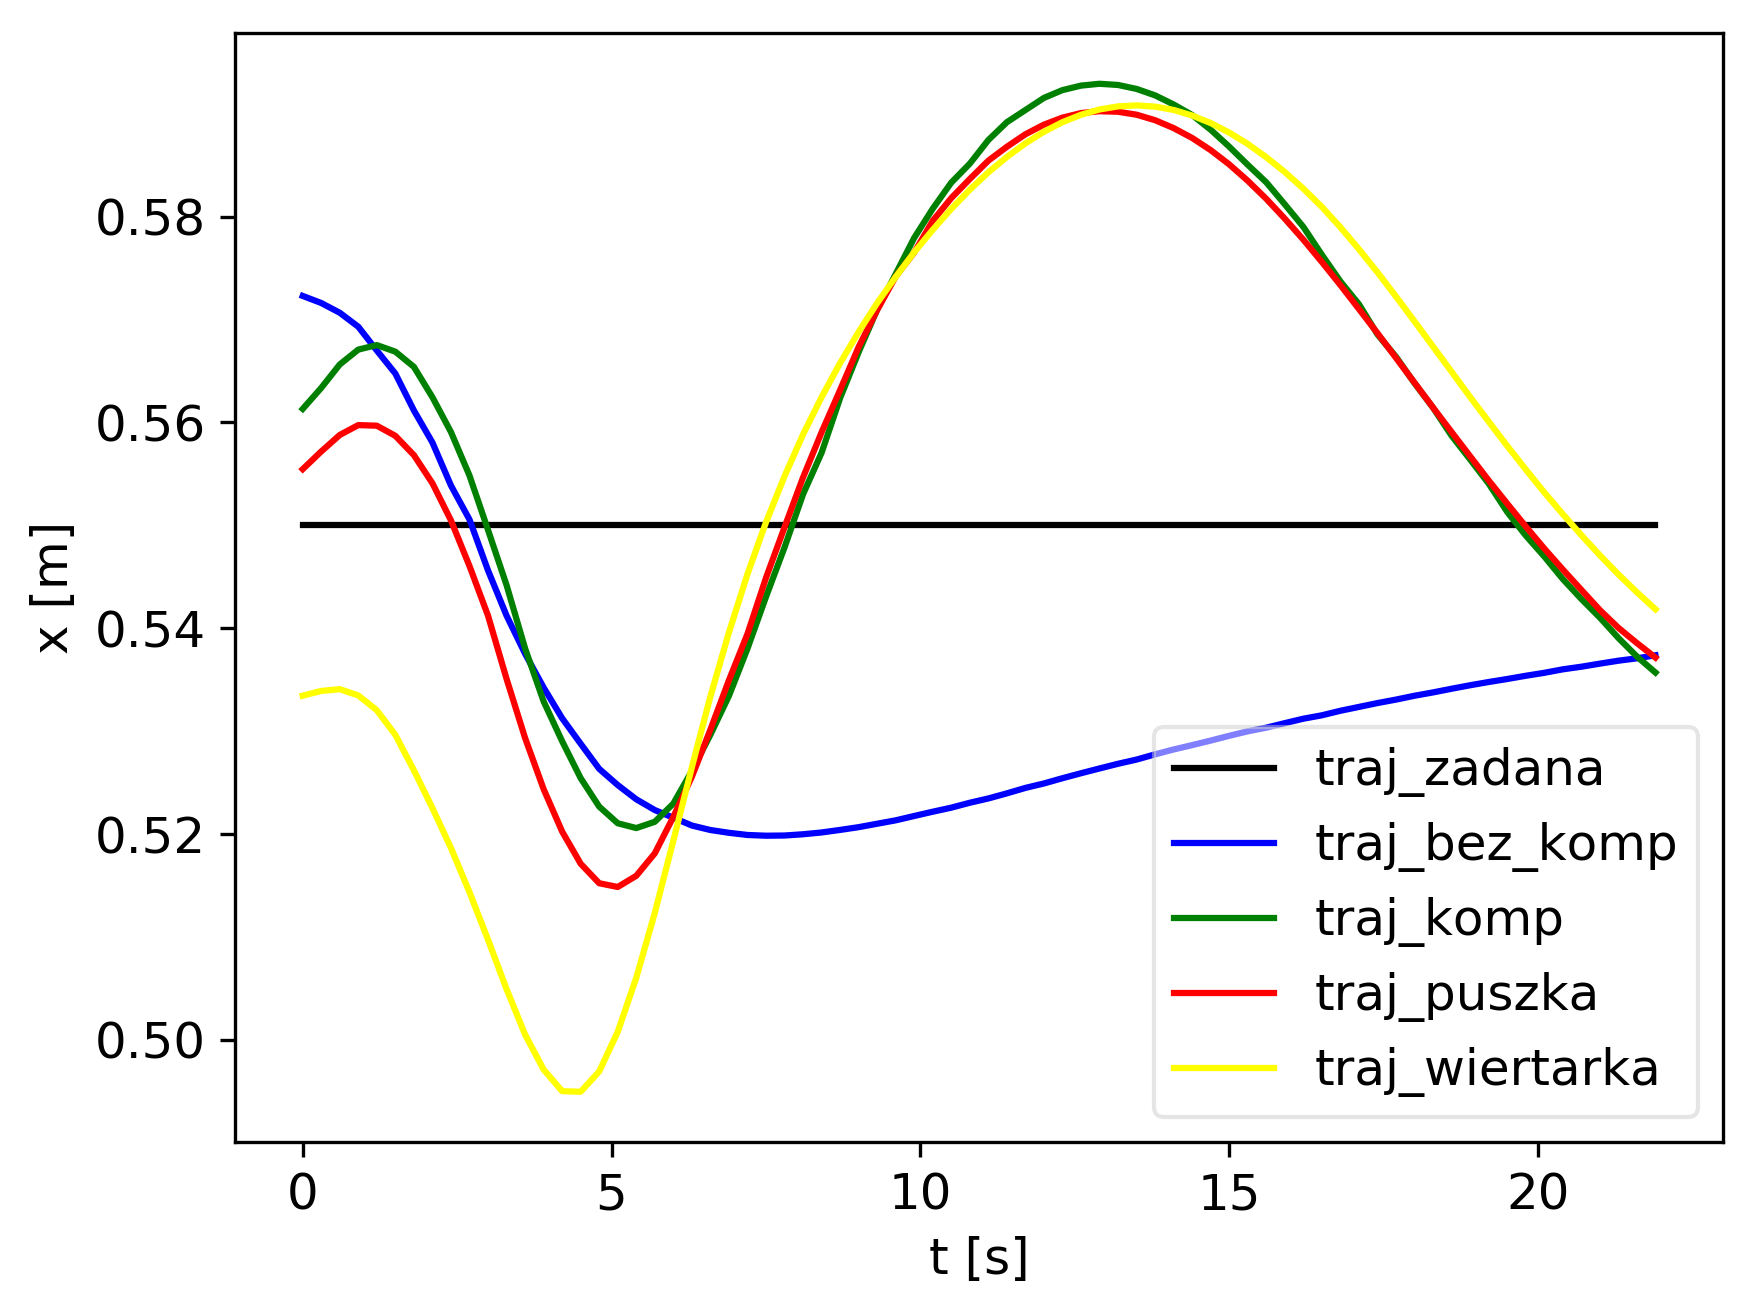
\includegraphics[width=.45\textwidth]{../../velma/przerobione_testy/out/w_bok_miekki/common_ax.png}
	}
	\hfill
	\subfigure[Os $Y$]{
		\label{fig:w_bok_miekki_ay}
		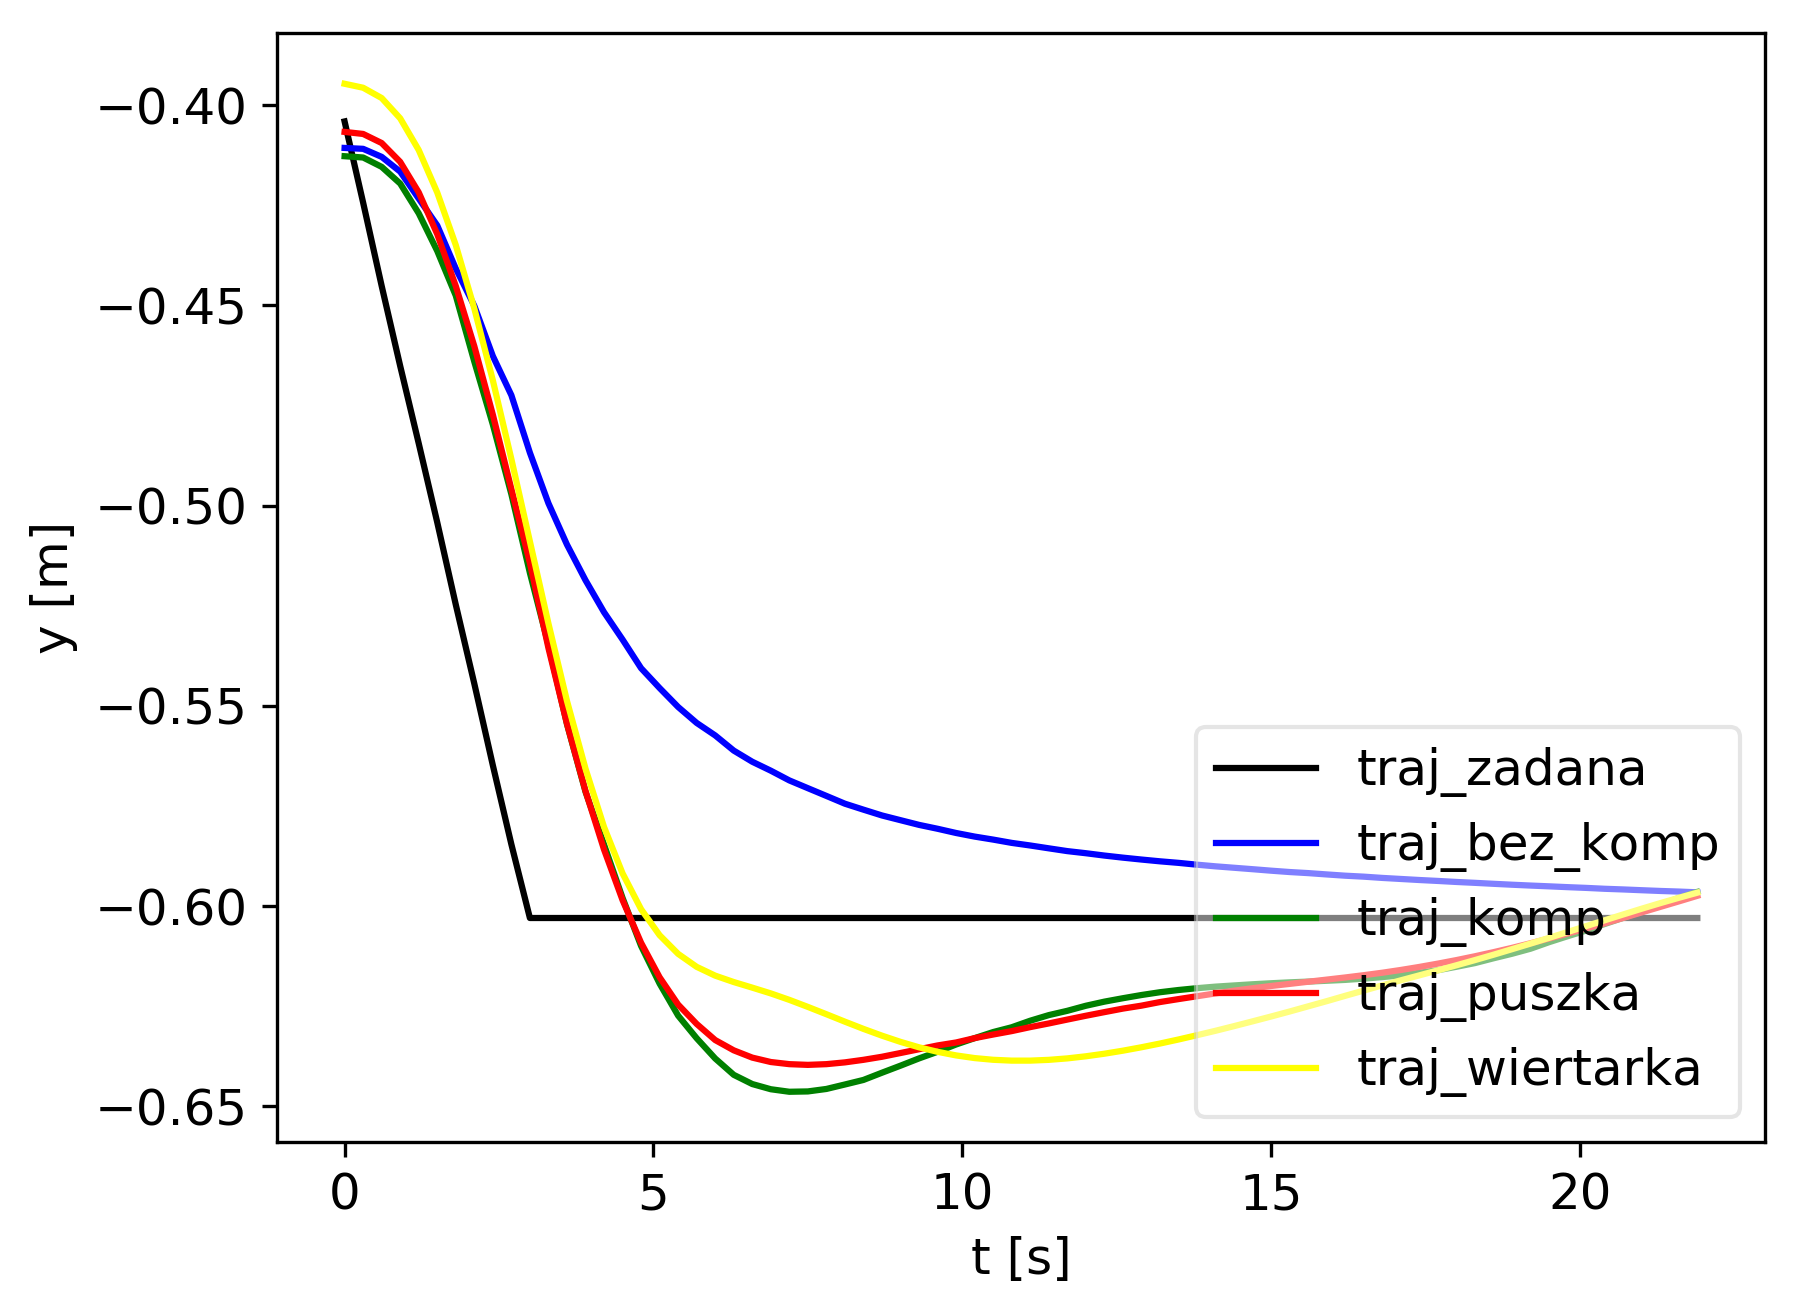
\includegraphics[width=.45\textwidth]{../../velma/przerobione_testy/out/w_bok_miekki/common_ay.png}
	}
	
	\hfill
	\subfigure[Os $Z$]{
		\label{fig:w_bok_miekki_az}
		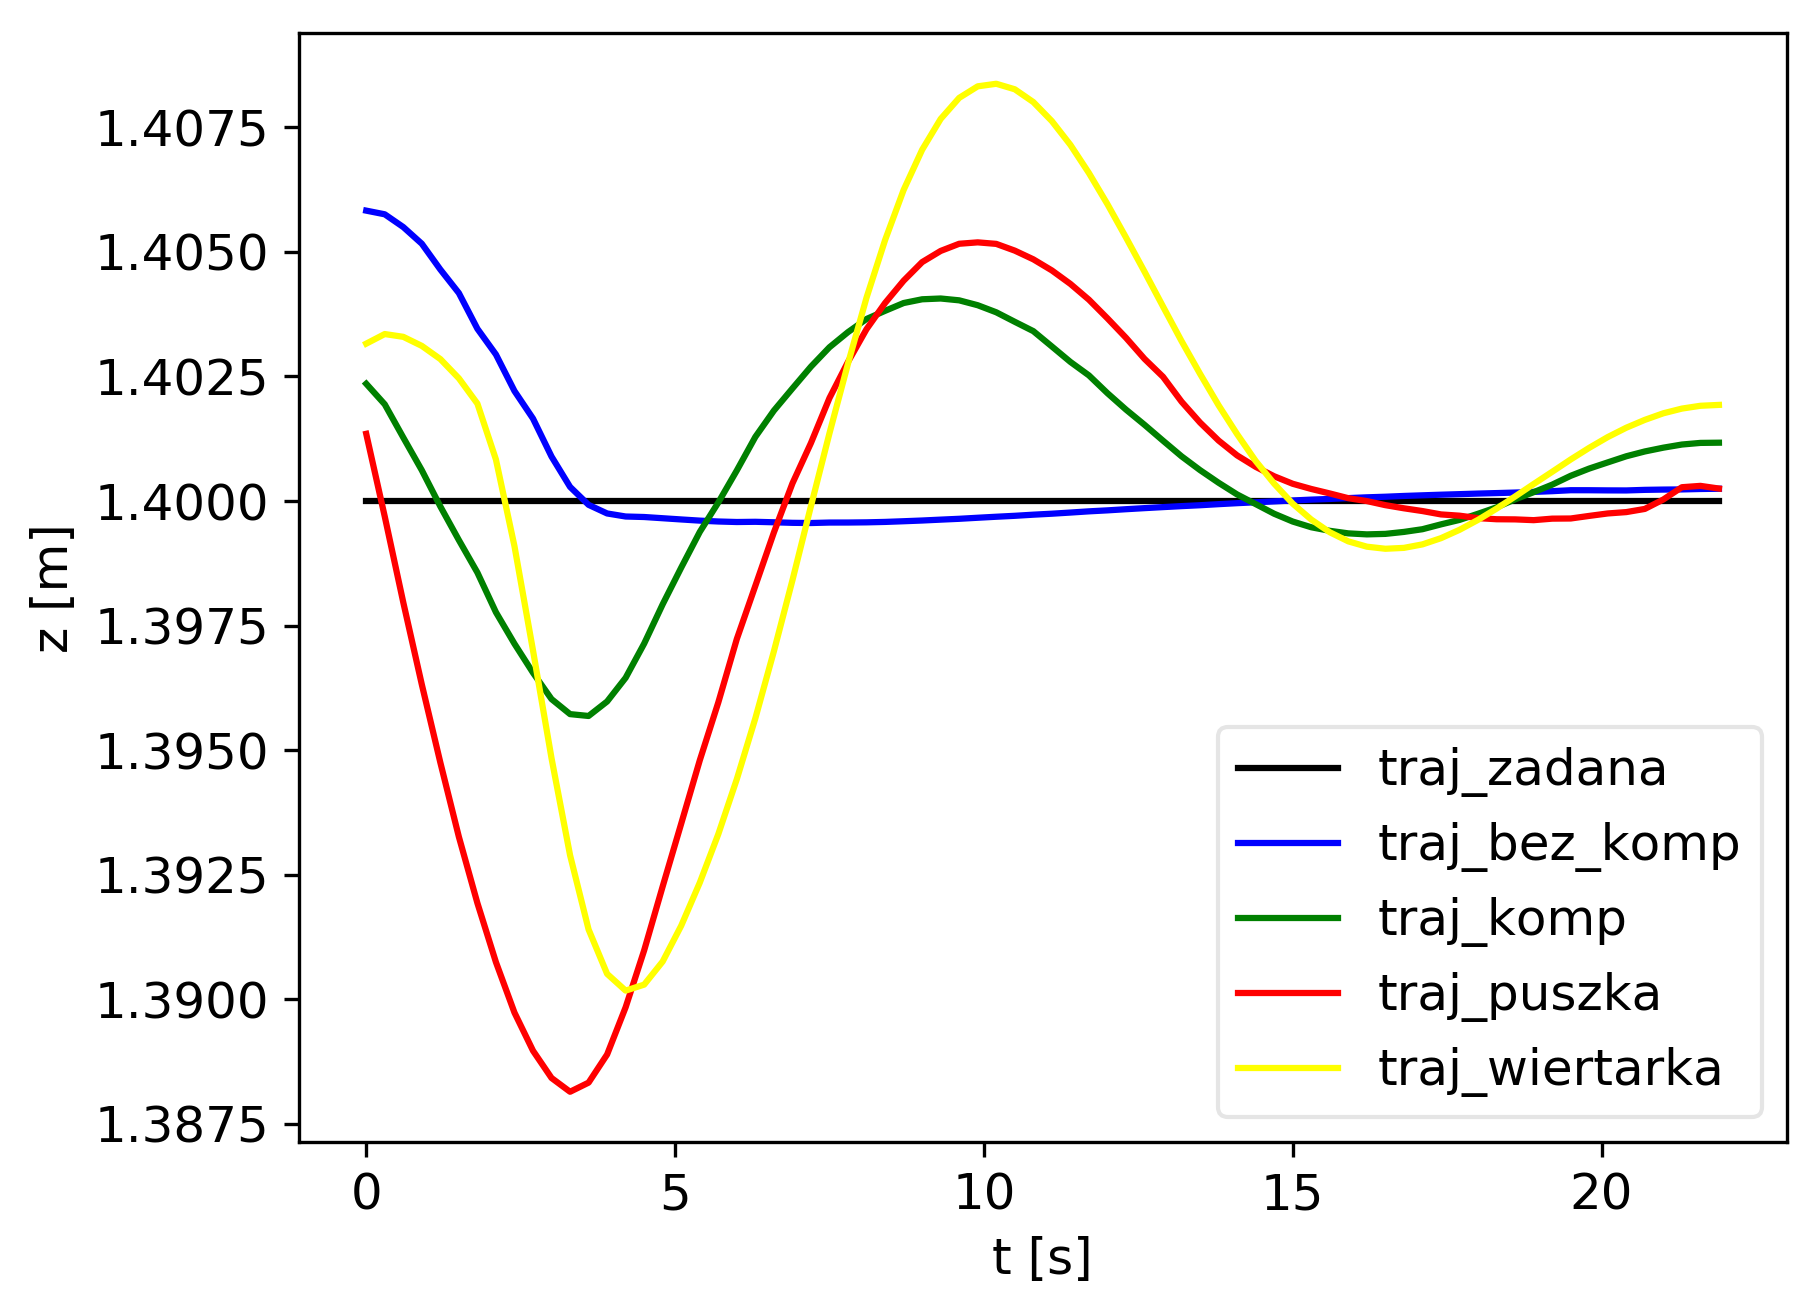
\includegraphics[width=.45\textwidth]{../../velma/przerobione_testy/out/w_bok_miekki/common_az.png}
	}

	\caption{Ruch do gory. Porownanie trajektorii pozycji w zaleznosci od czasu.}
	\label{fig:w_bok_miekki_a}

\end{figure}


\begin{figure}[h]
	\centering
	\subfigure[Kat osi $X$]{
		\label{fig:w_bok_miekki_rotx}
		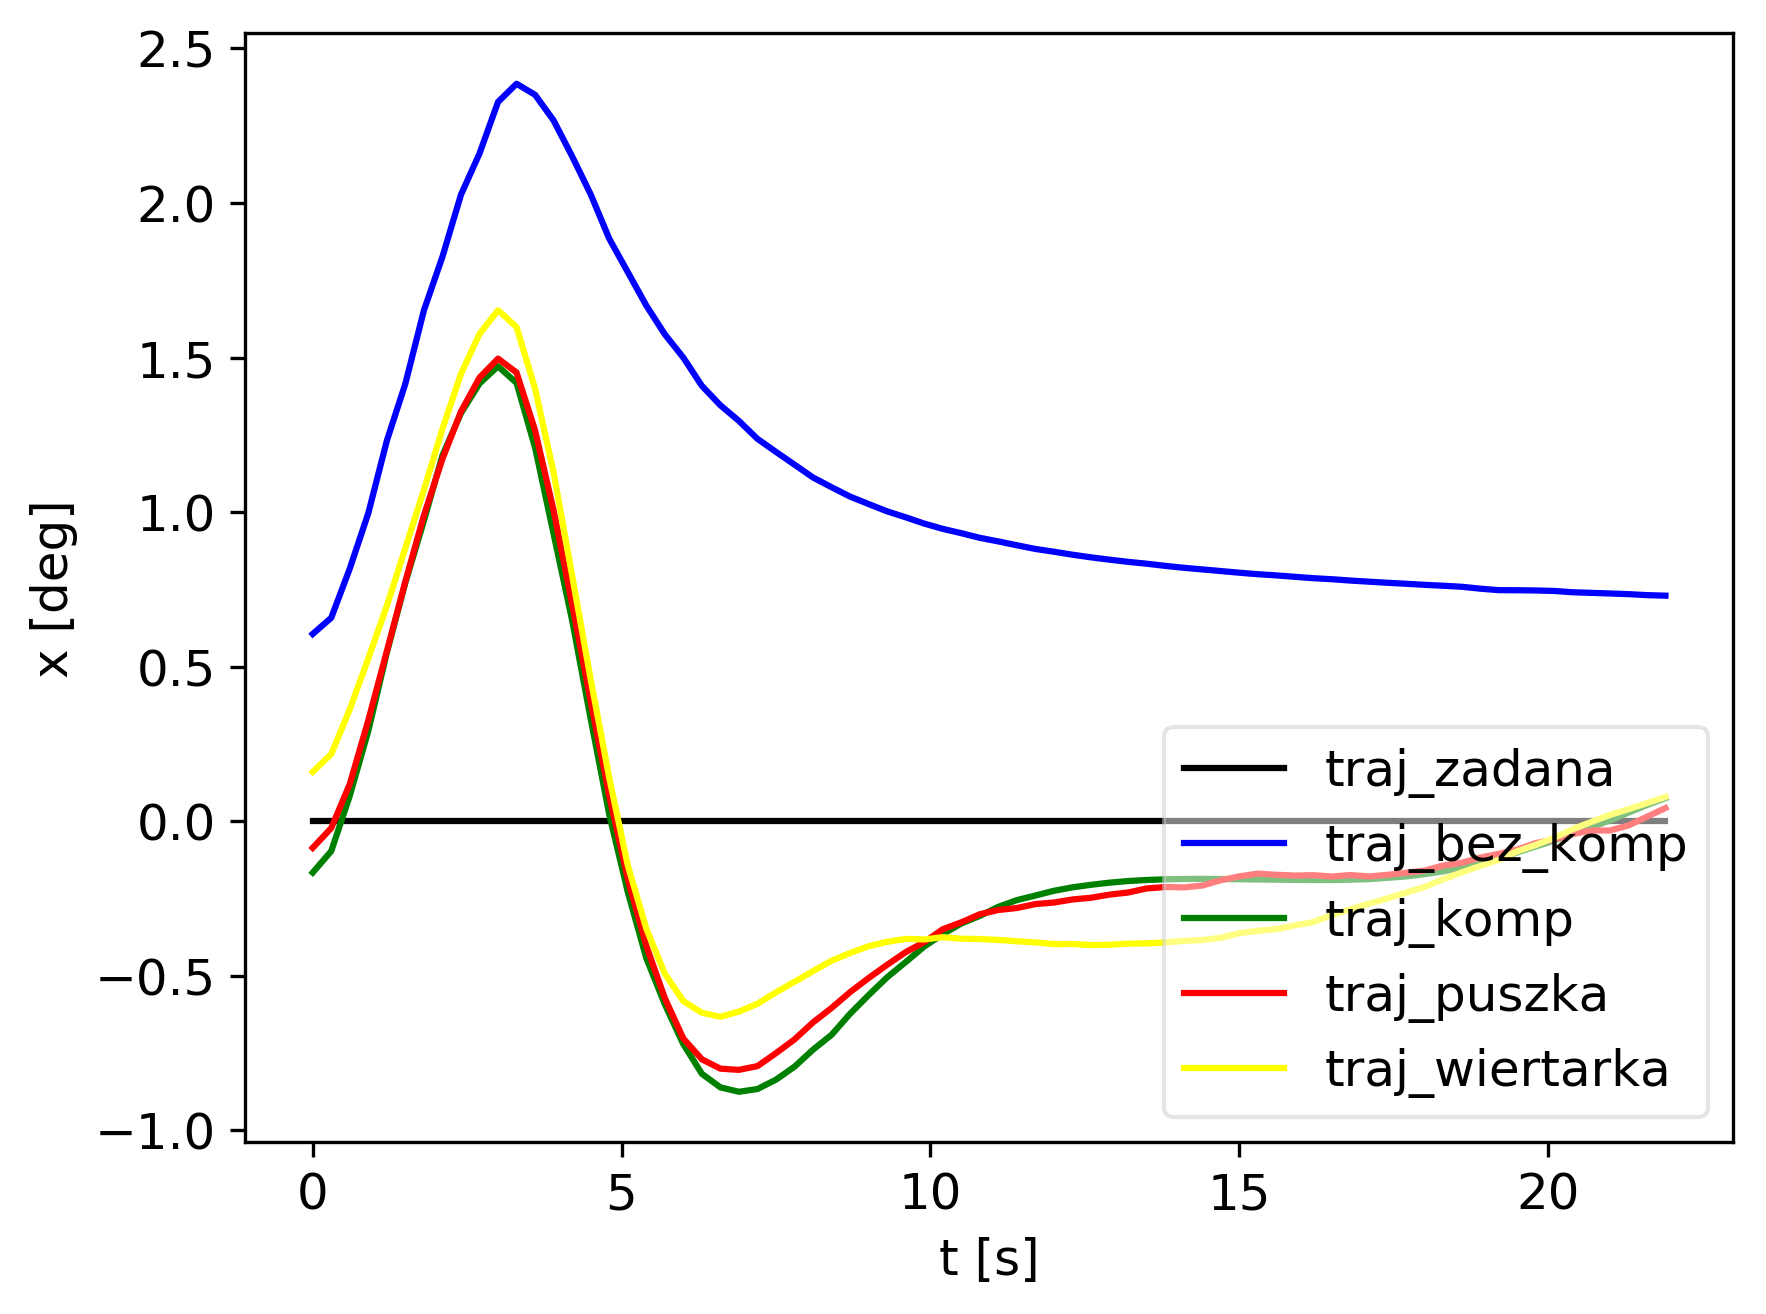
\includegraphics[width=.45\textwidth]{../../velma/przerobione_testy/out/w_bok_miekki/common_rotx.png}
	}
	\hfill
	\subfigure[Kat osi $Y$]{
		\label{fig:w_bok_miekki_roty}
		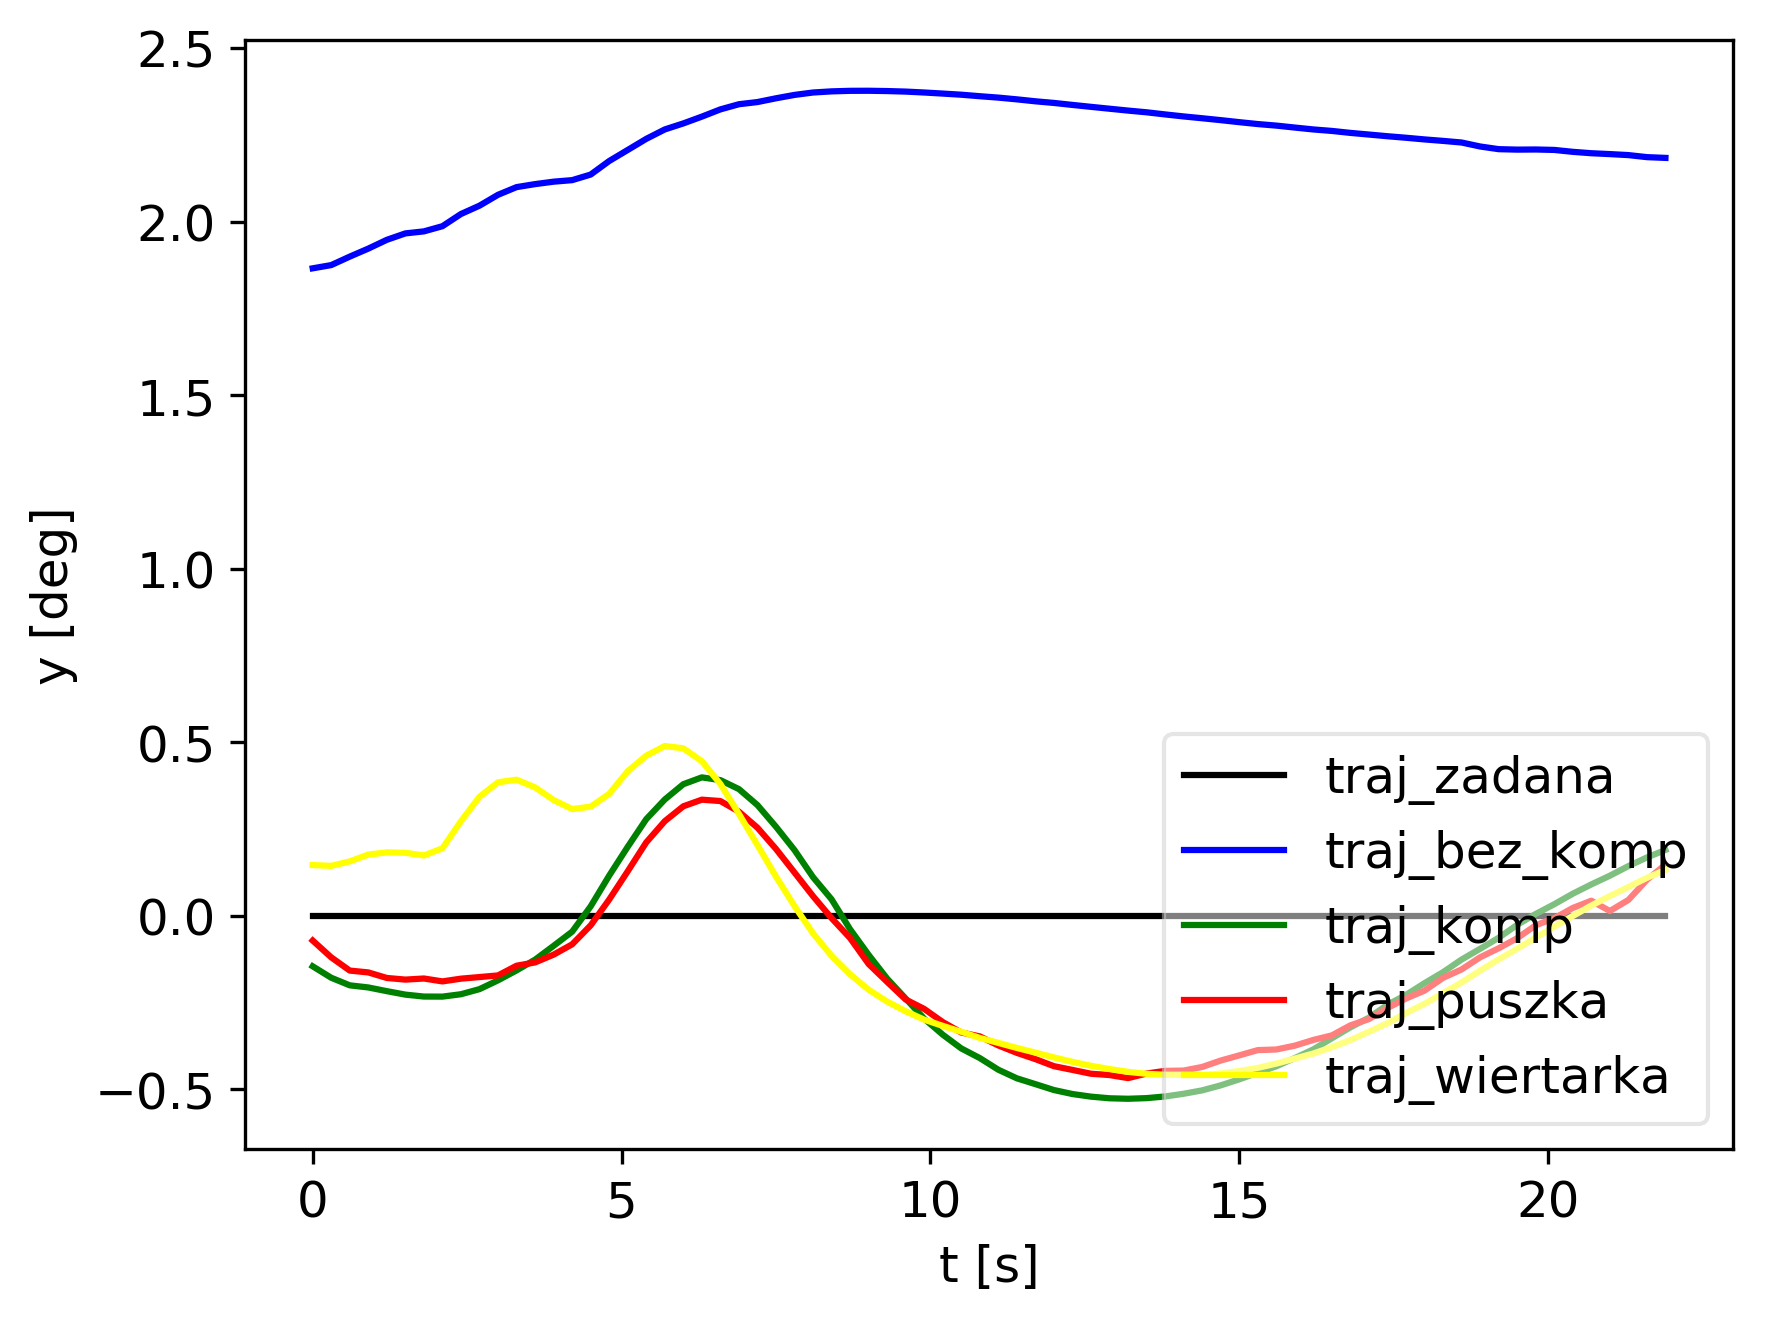
\includegraphics[width=.45\textwidth]{../../velma/przerobione_testy/out/w_bok_miekki/common_roty.png}
	}
	
	\hfill
	\subfigure[Kat osi $Z$]{
		\label{fig:w_bok_miekki_rotz}
		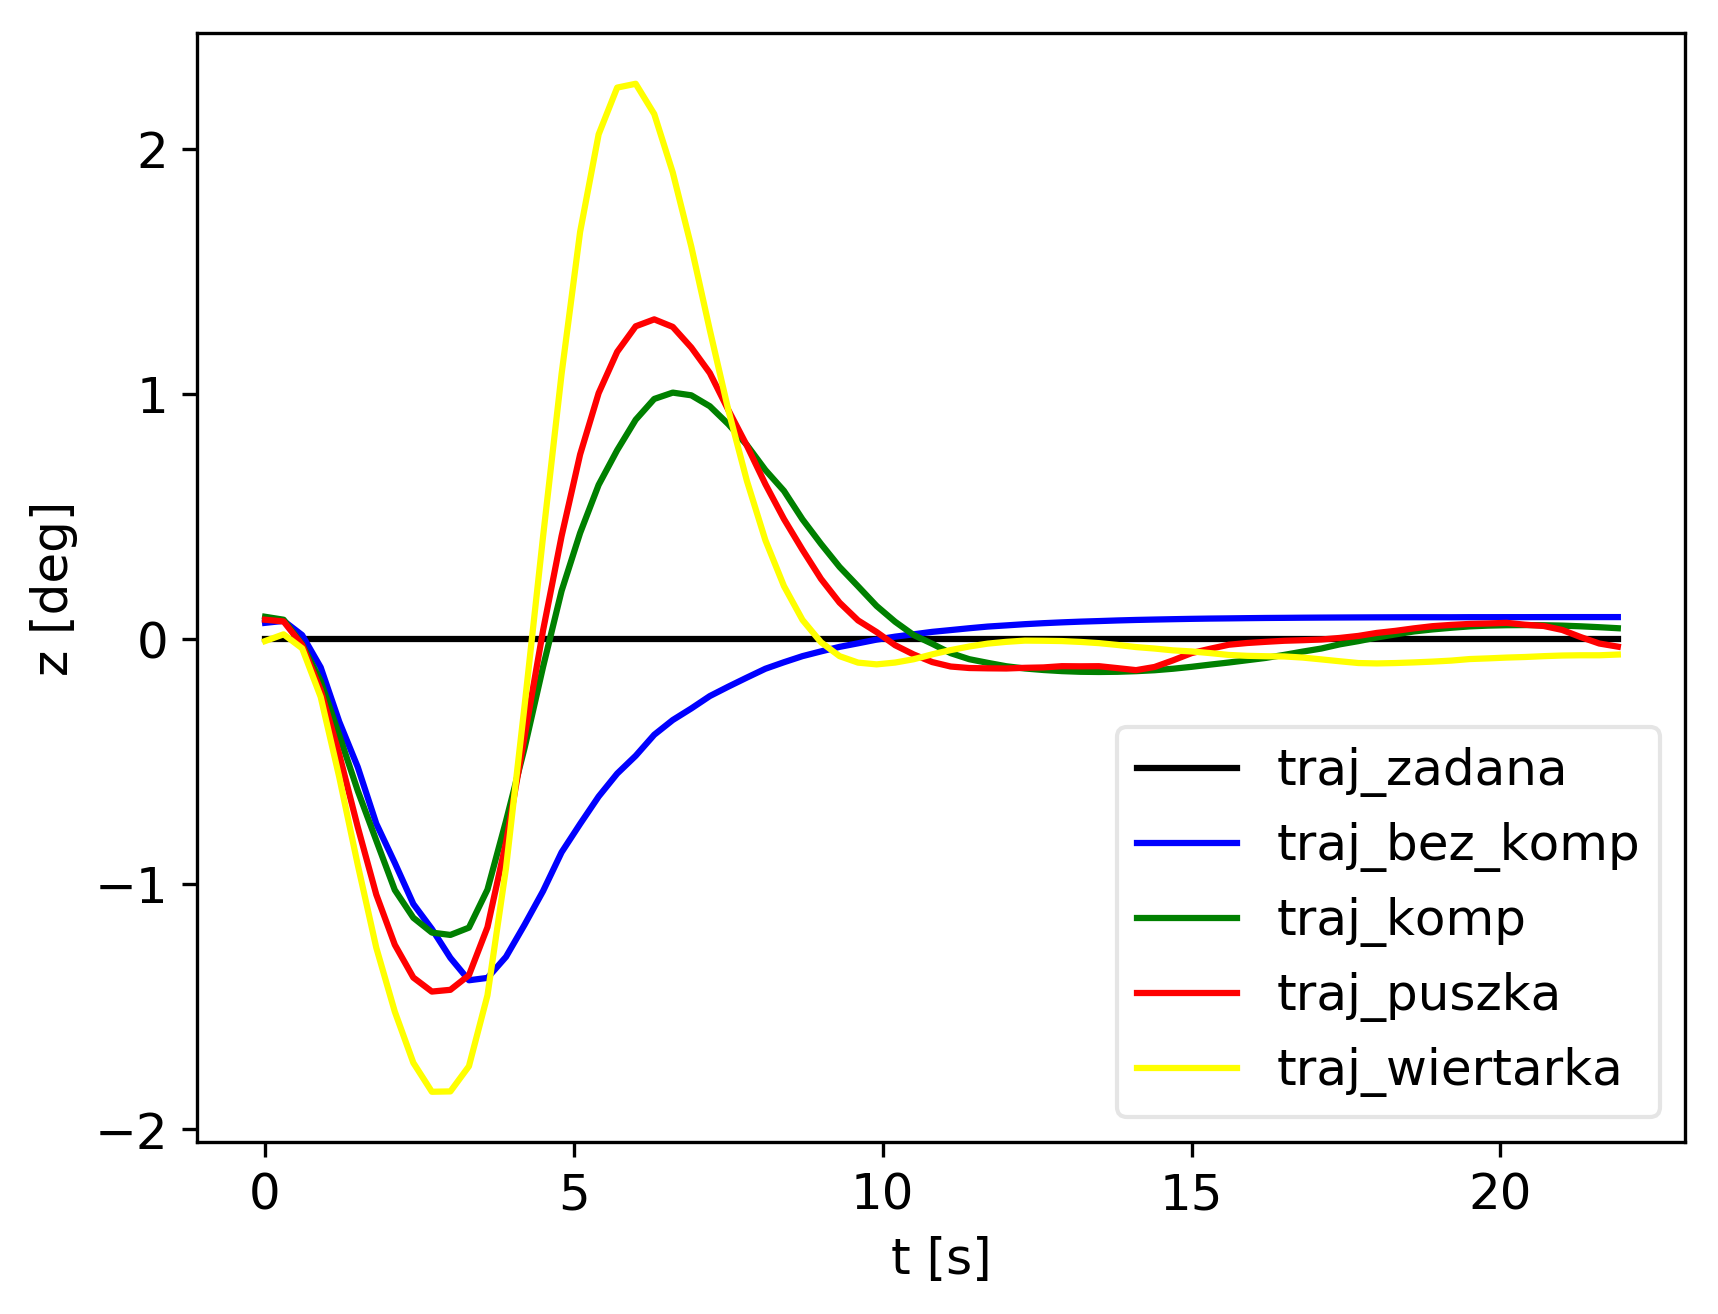
\includegraphics[width=.45\textwidth]{../../velma/przerobione_testy/out/w_bok_miekki/common_rotz.png}
	}

	\caption{Ruch do gory. Porownanie trajektorii katow w notacji Eulera w zaleznosci od czasu.}
	\label{fig:w_bok_miekki_rot}

\end{figure}


\begin{figure}[h]
	\centering
	\subfigure[Brak algorytmu kompensacji]{
		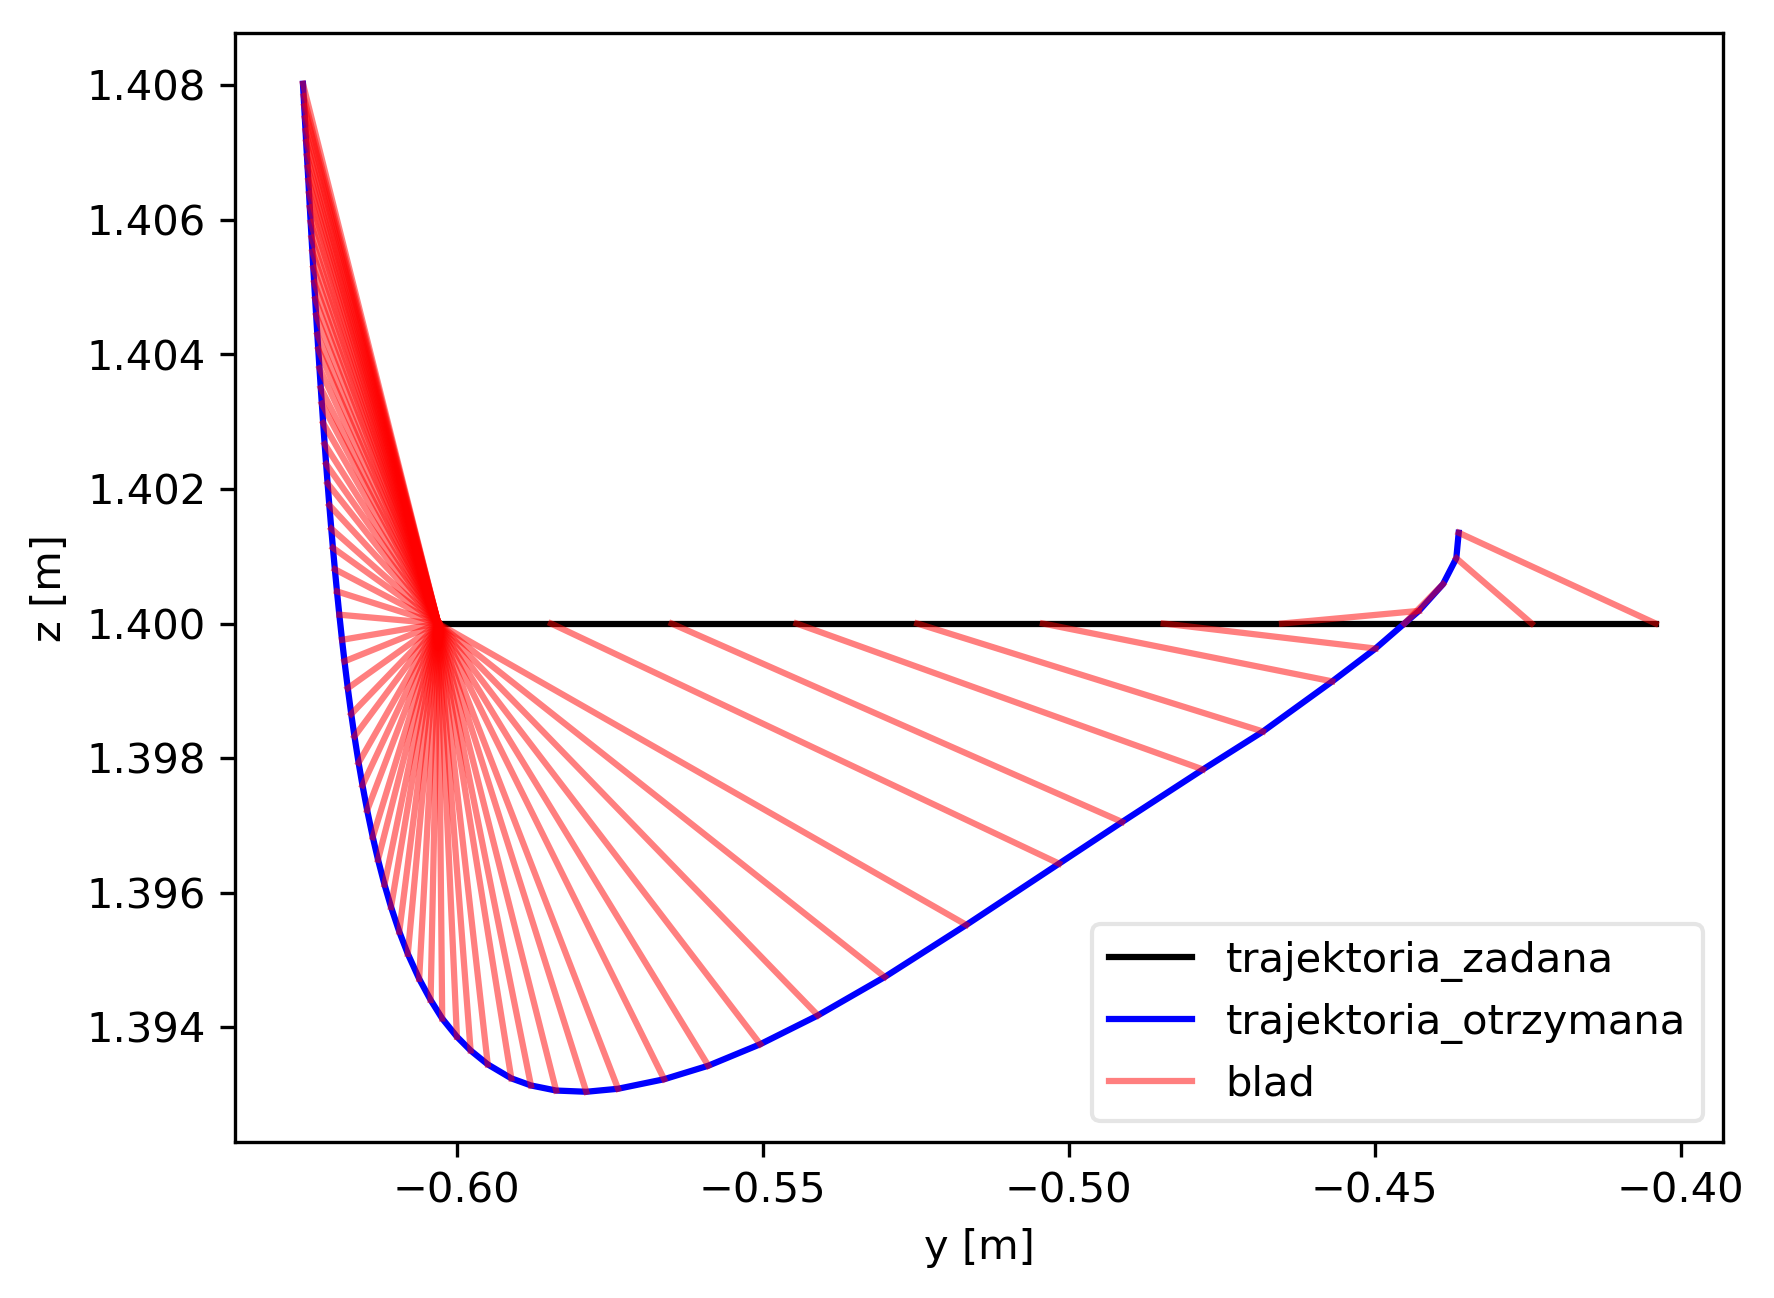
\includegraphics[width=.45\textwidth]{../../velma/przerobione_testy/out/w_bok_miekki/yz_ate_plot_podnoszenie_miekki_bez_brak.png}
	}
	\hfill
	\subfigure[Zalaczony algorytm kompnesacji]{
		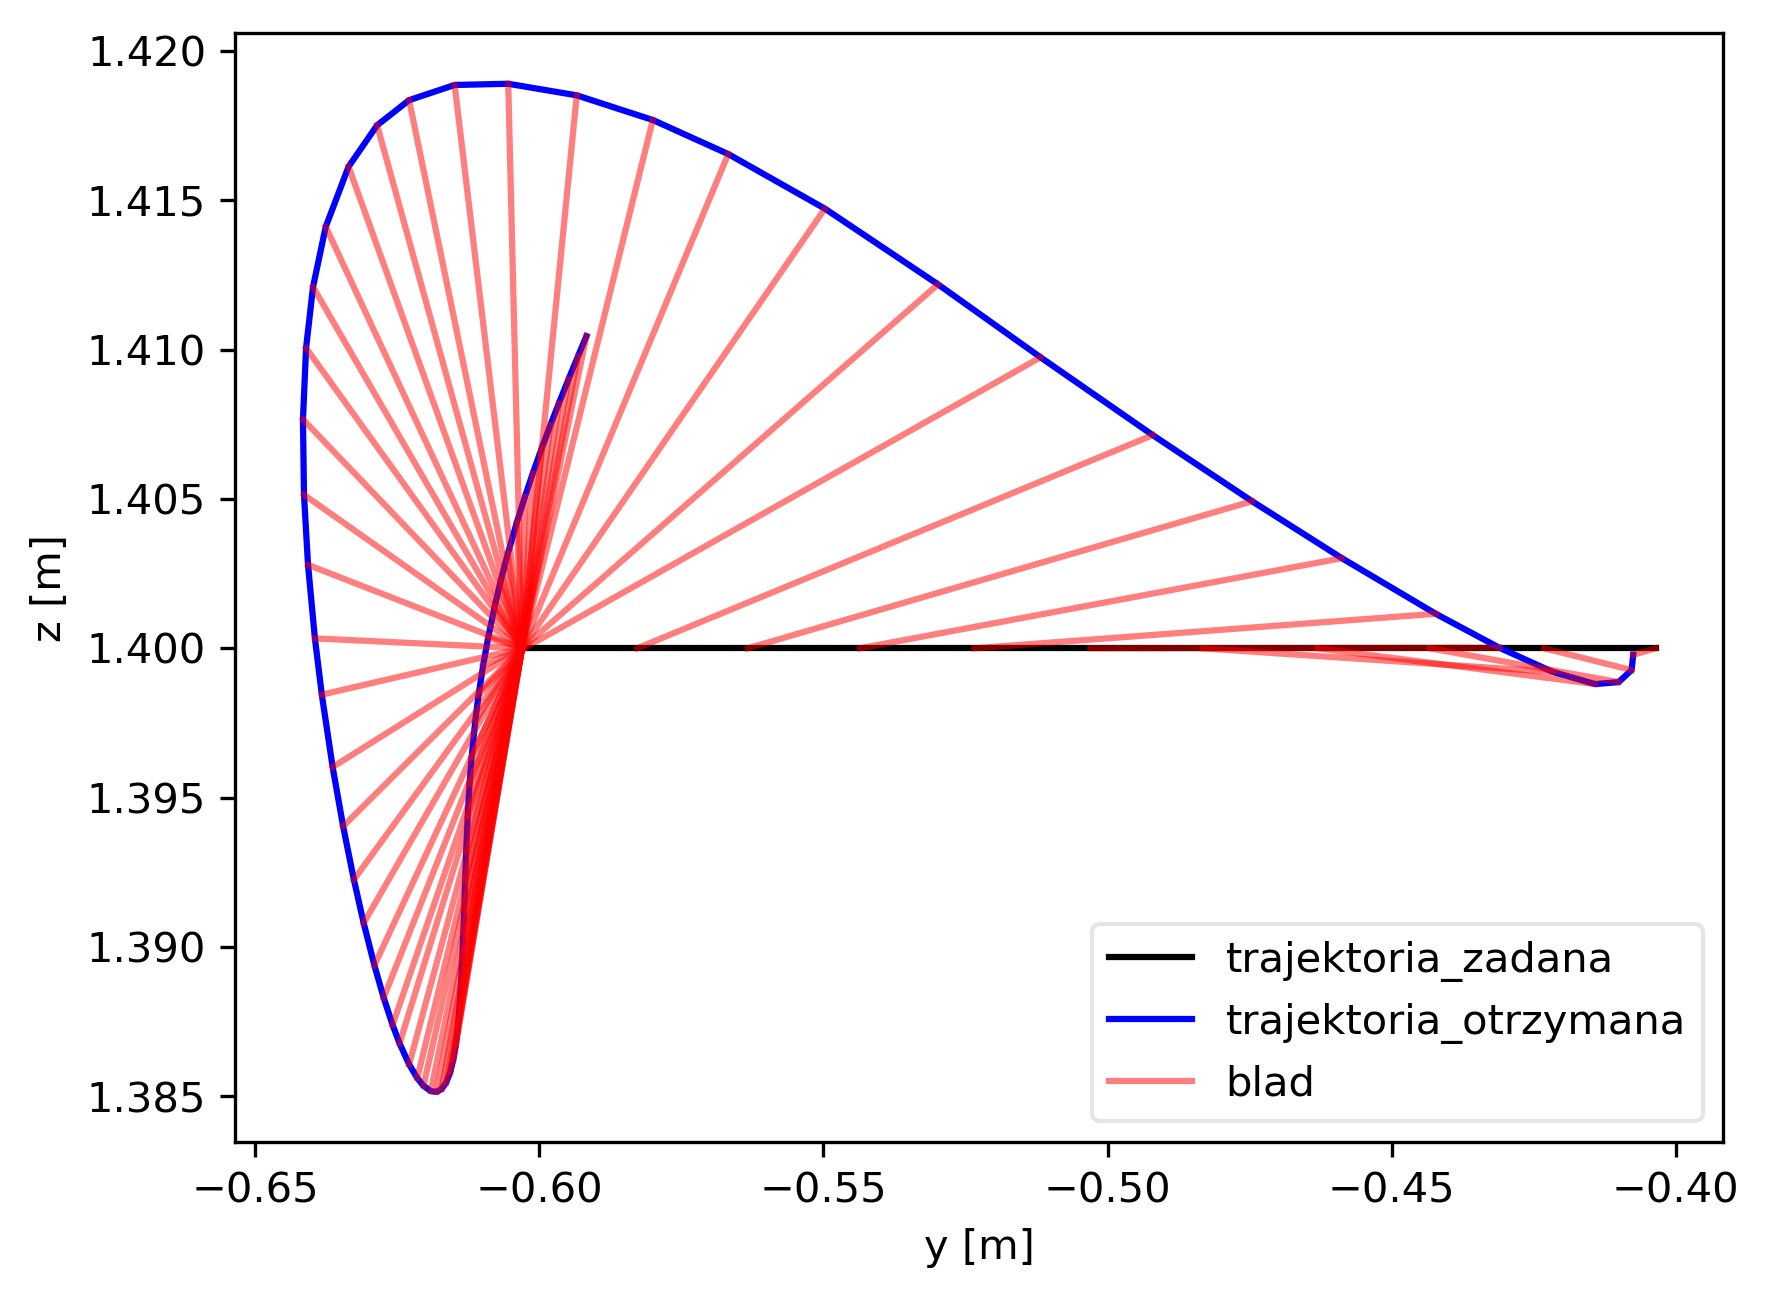
\includegraphics[width=.45\textwidth]{../../velma/przerobione_testy/out/w_bok_miekki/yz_ate_plot_podnoszenie_miekki_komp_brak.png}
	}
	\caption{Porownanie trajektorii chwytaka w osiach $Y$ i $Z$}
	\label{fig:w_bok_miekki_porow_komp}
\end{figure}

\begin{figure}[h]
	\centering
	\subfigure[Trajektoria z chwycona puszka]{
		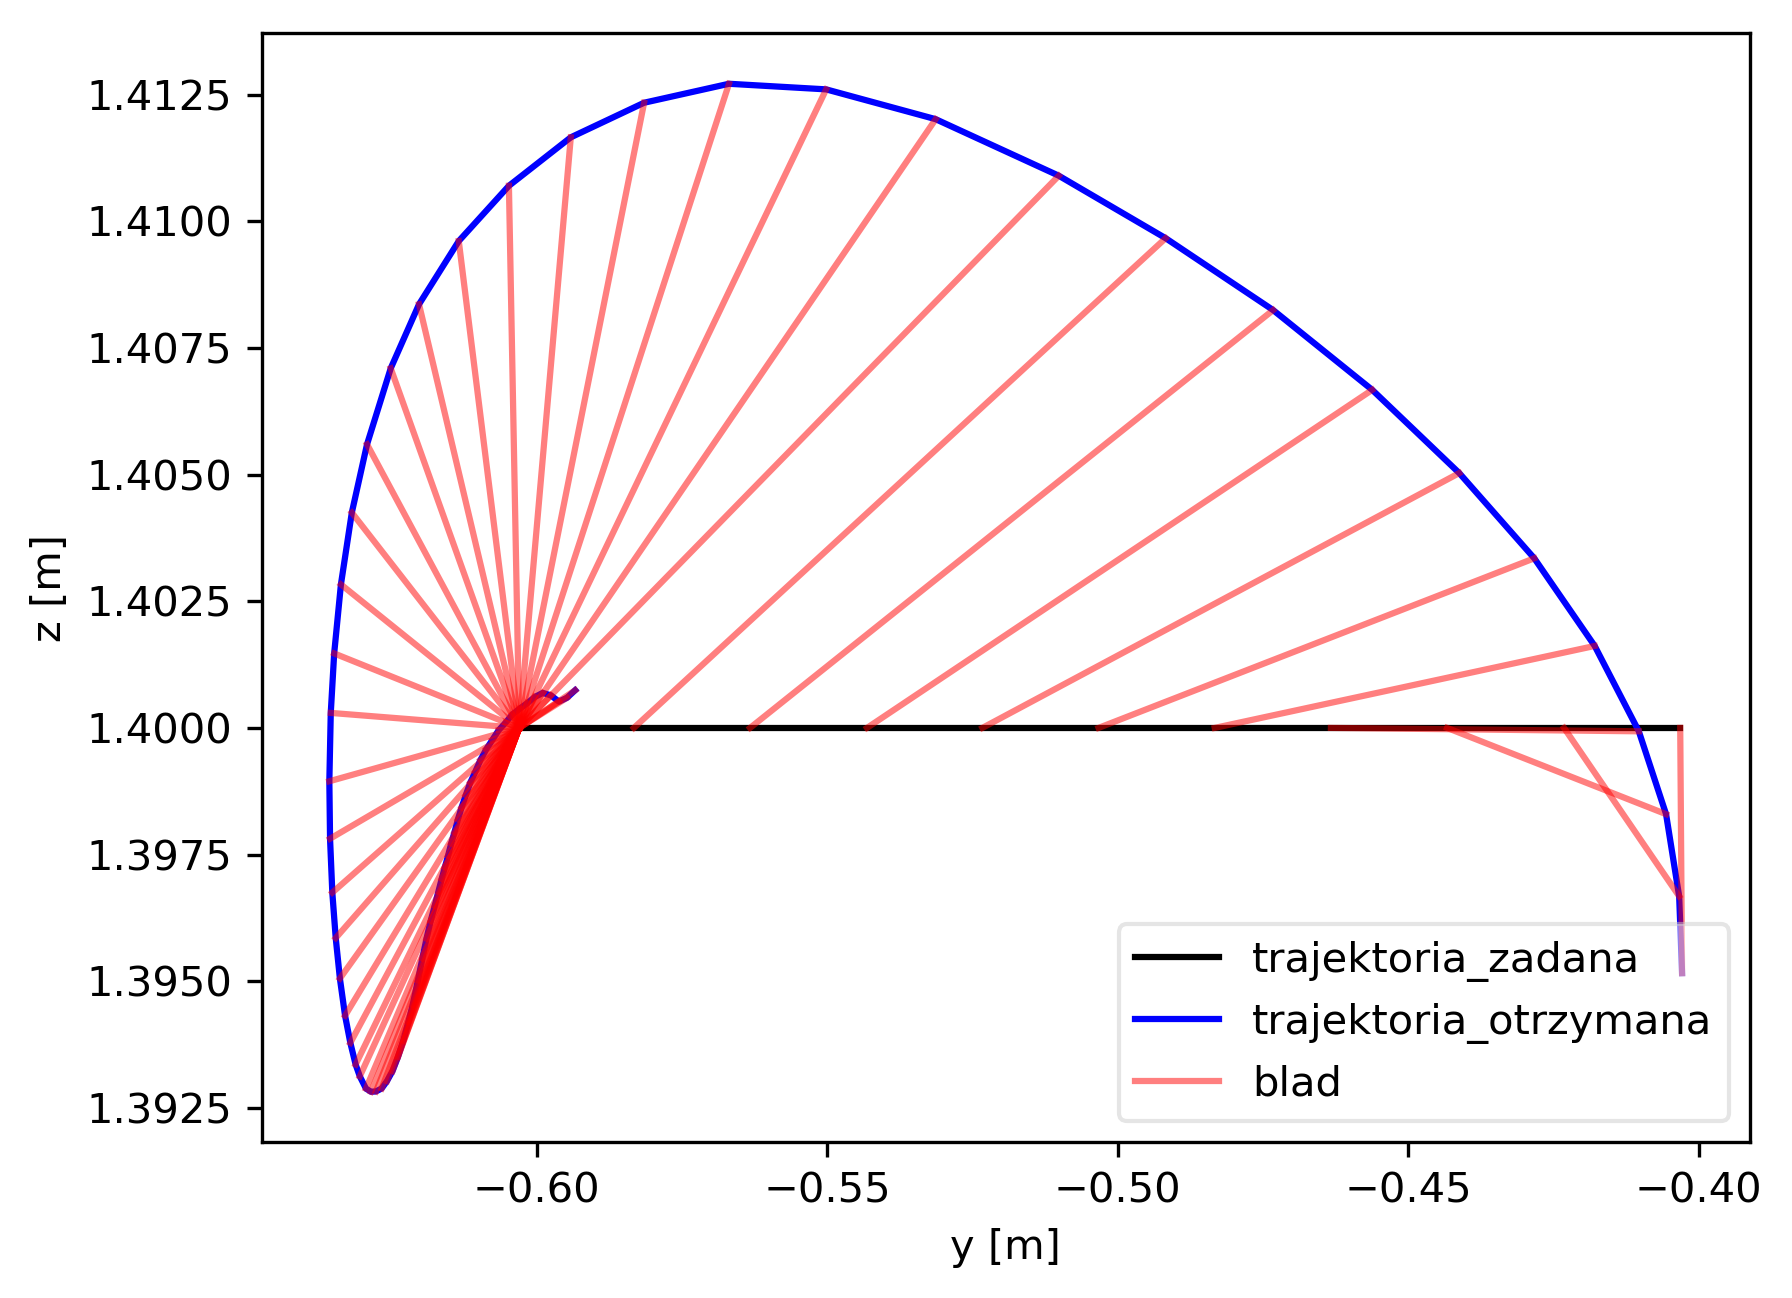
\includegraphics[width=.45\textwidth]{../../velma/przerobione_testy/out/w_bok_miekki/yz_ate_plot_podnoszenie_miekki_komp_piwo.png}
	}
	\hfill
	\subfigure[Trajektoria z chwycona wiertarka]{
		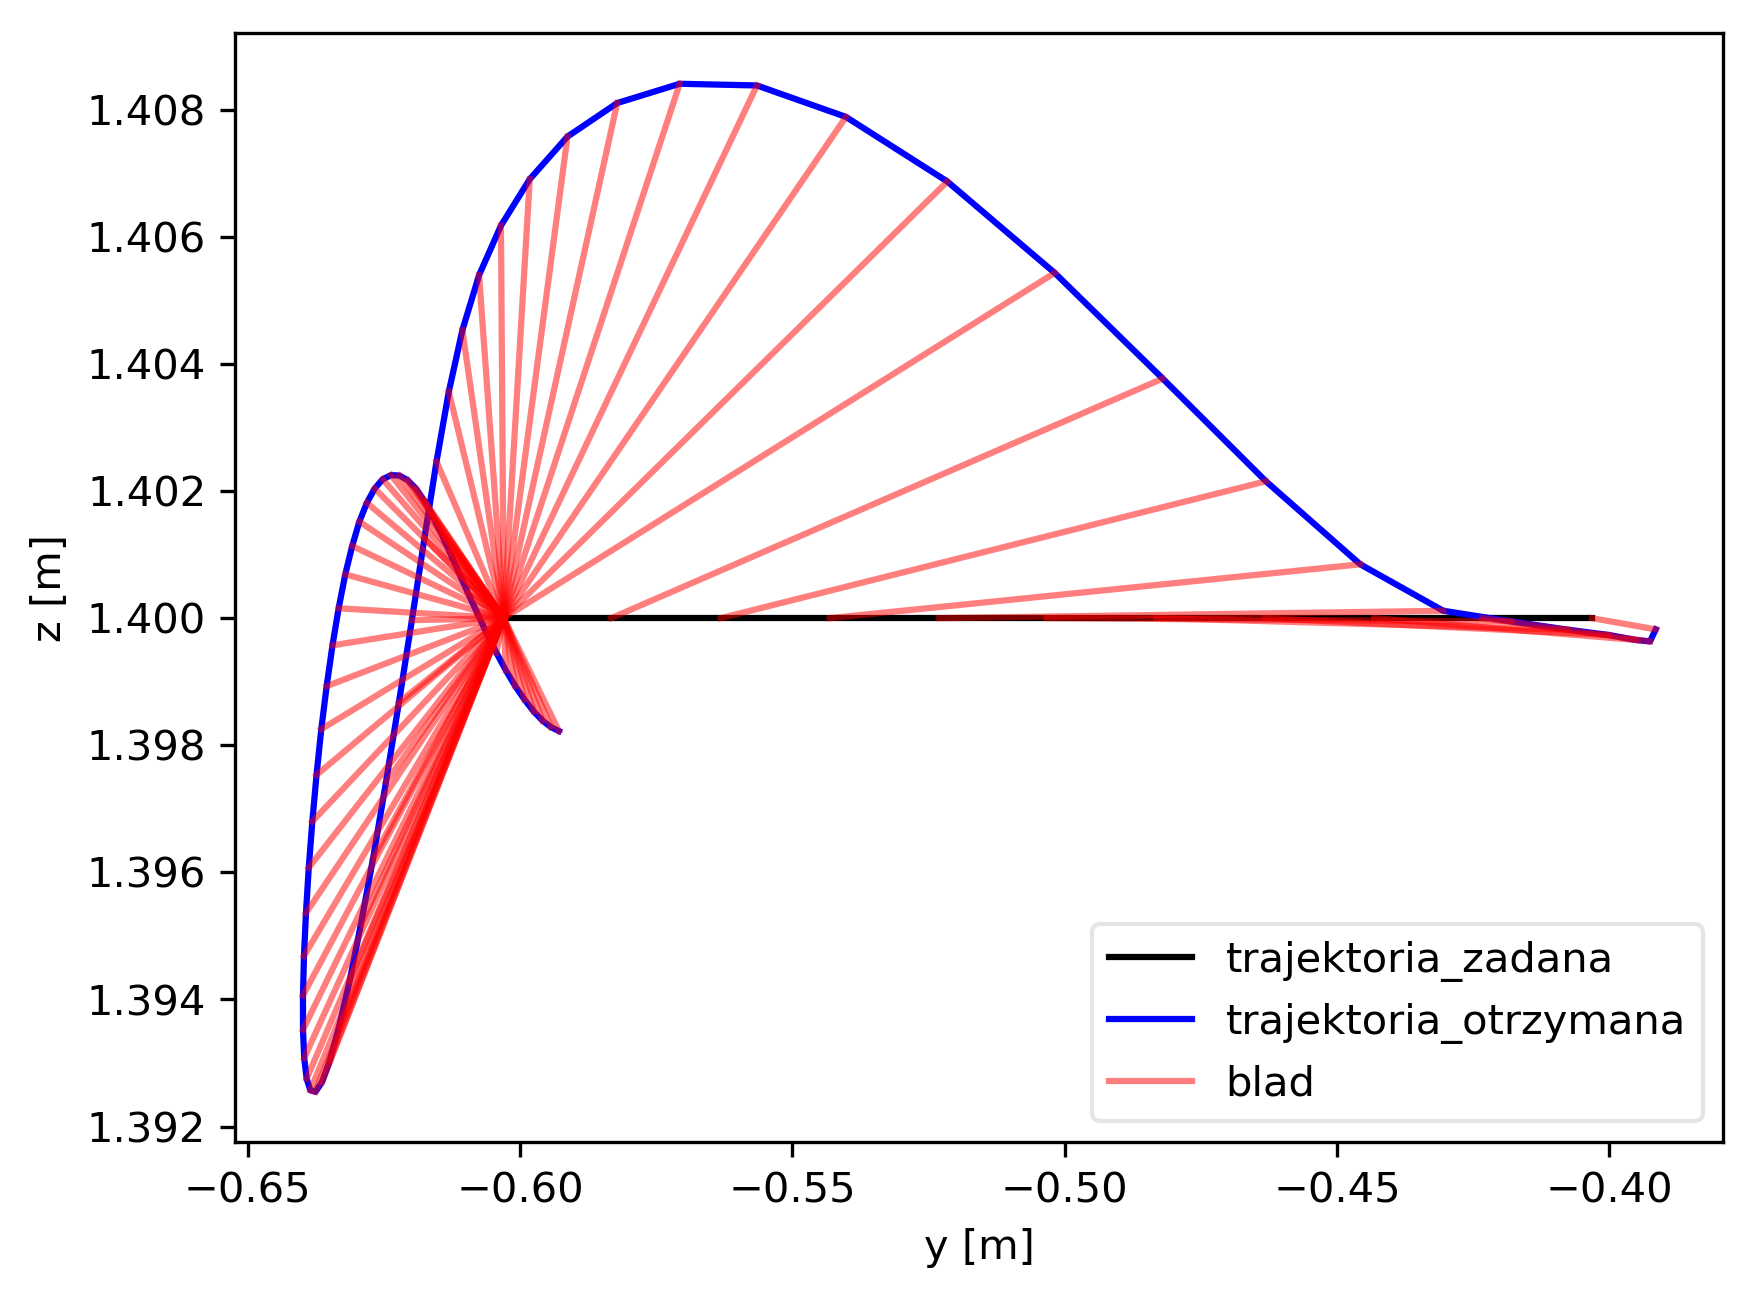
\includegraphics[width=.45\textwidth]{../../velma/przerobione_testy/out/w_bok_miekki/yz_ate_plot_podnoszenie_miekki_komp_wiertarka.png}
	}
	\caption{Porownanie trajektorii chwytaka w osiach $Y$ i $Z$}
	\label{fig:w_bok_miekki_porow_przedm}
\end{figure}


% \begin{figure}
% 	\centering
% 	\subfigure[Brak algorytmu kompensacji]{
% 		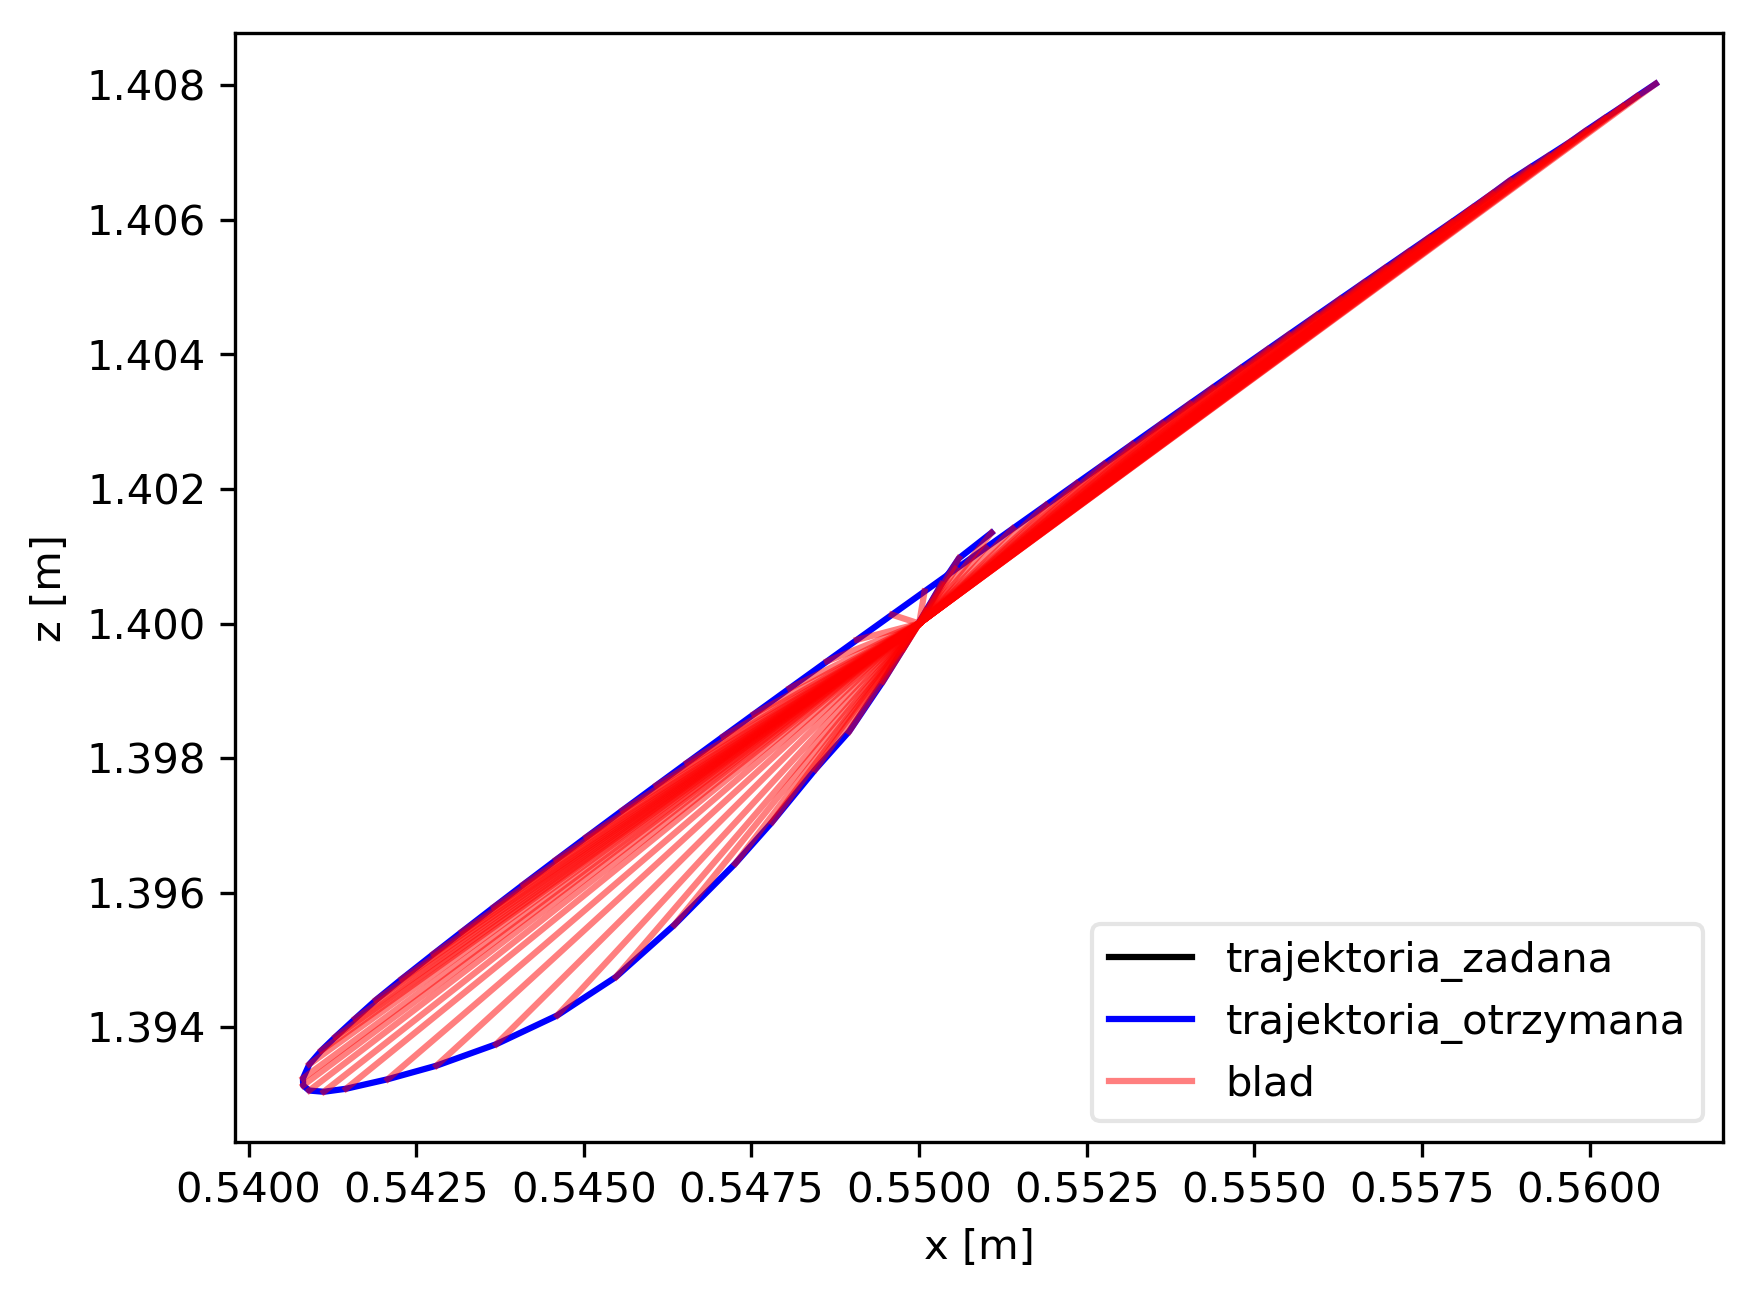
\includegraphics[width=.45\textwidth]{../../velma/przerobione_testy/out/w_bok_miekki/xz_ate_plot_podnoszenie_miekki_bez_brak.png}
% 	}
% 	\hfill
% 	\subfigure[Zalaczony algorytm kompnesacji]{
% 		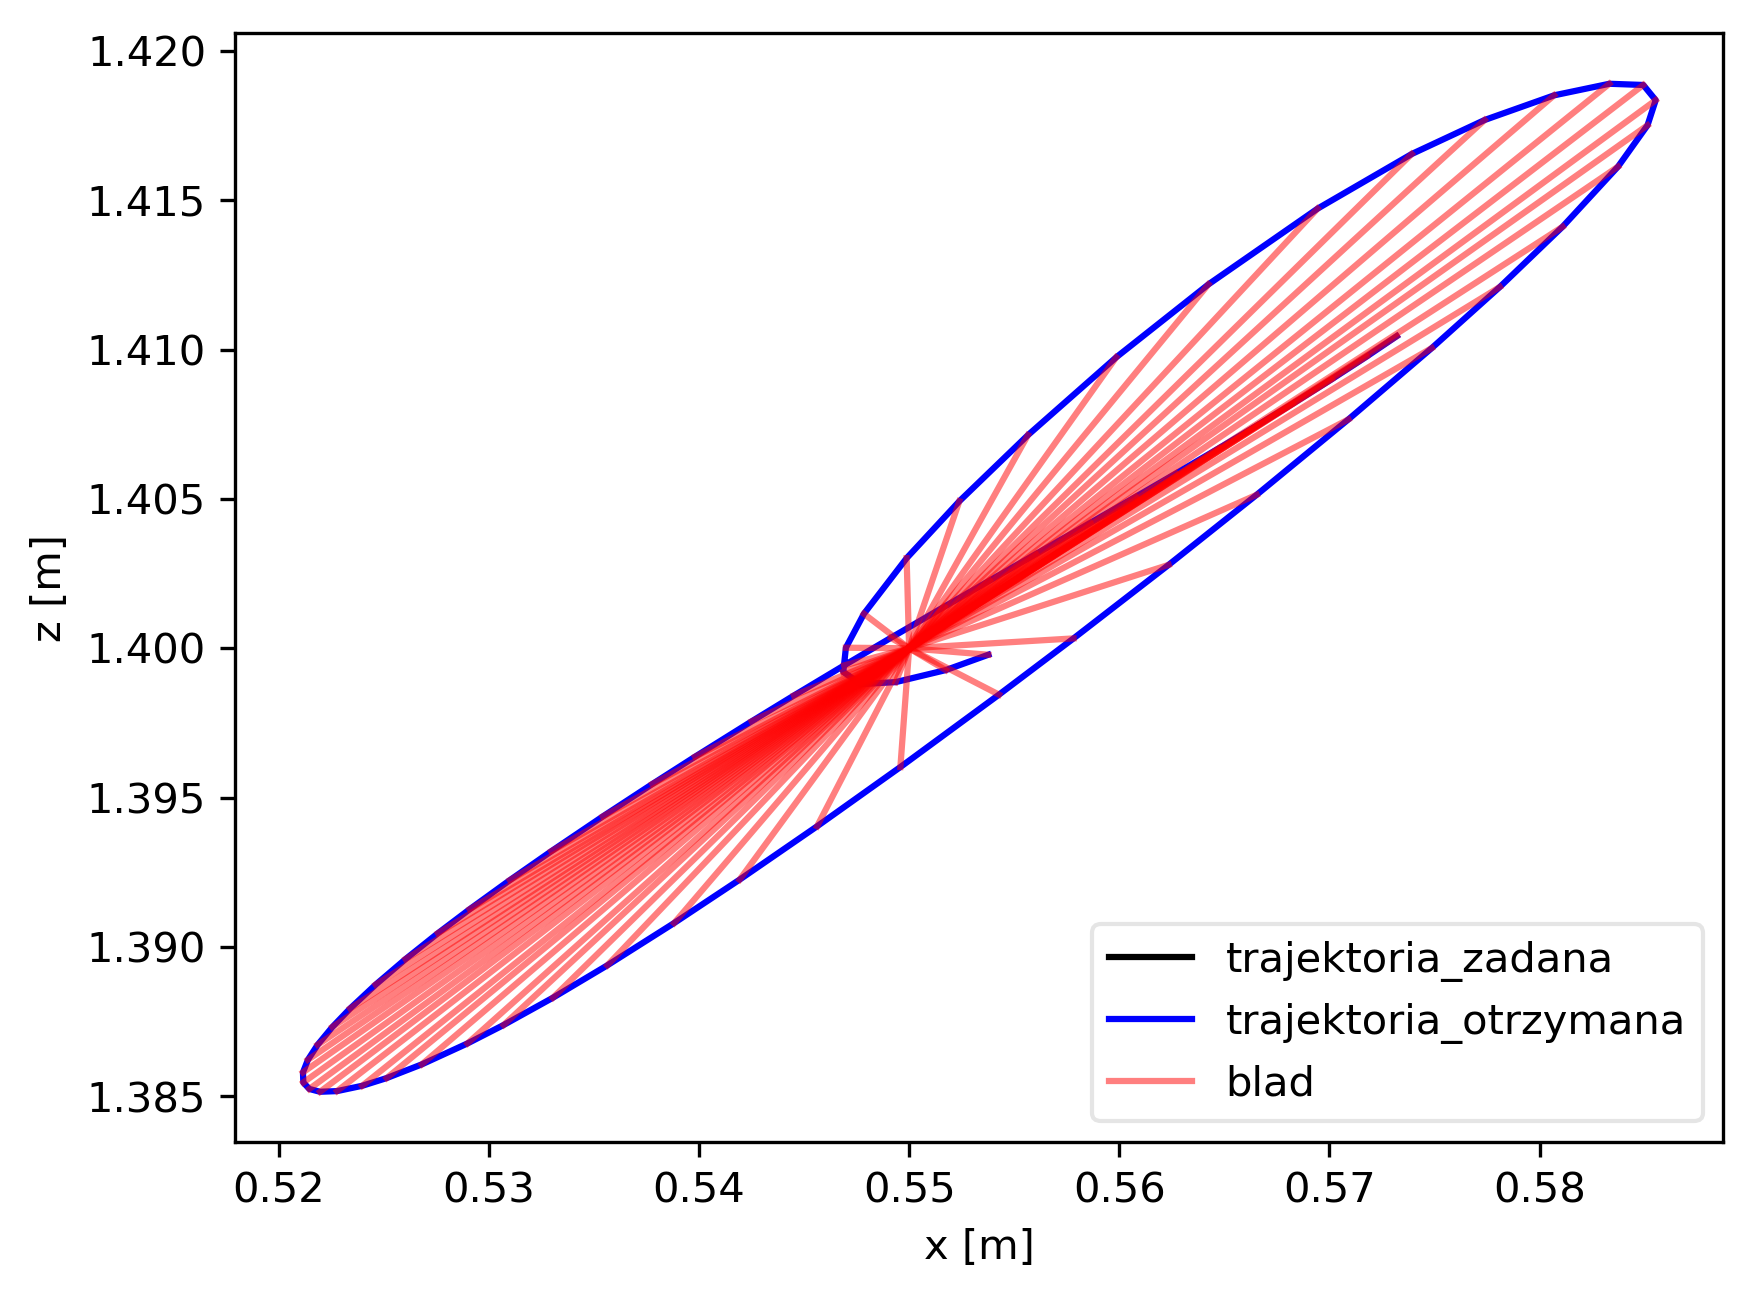
\includegraphics[width=.45\textwidth]{../../velma/przerobione_testy/out/w_bok_miekki/xz_ate_plot_podnoszenie_miekki_komp_brak.png}
% 	}
% 	\caption{Porownanie trajektorii chwytaka w osiach $X$ i $Z$}
% 	\label{fig:w_bok_miekki_porow_komp_bok}
% \end{figure}

% \begin{figure}
% 	\centering
% 	\subfigure[Trajektoria z chwycona puszka]{
% 		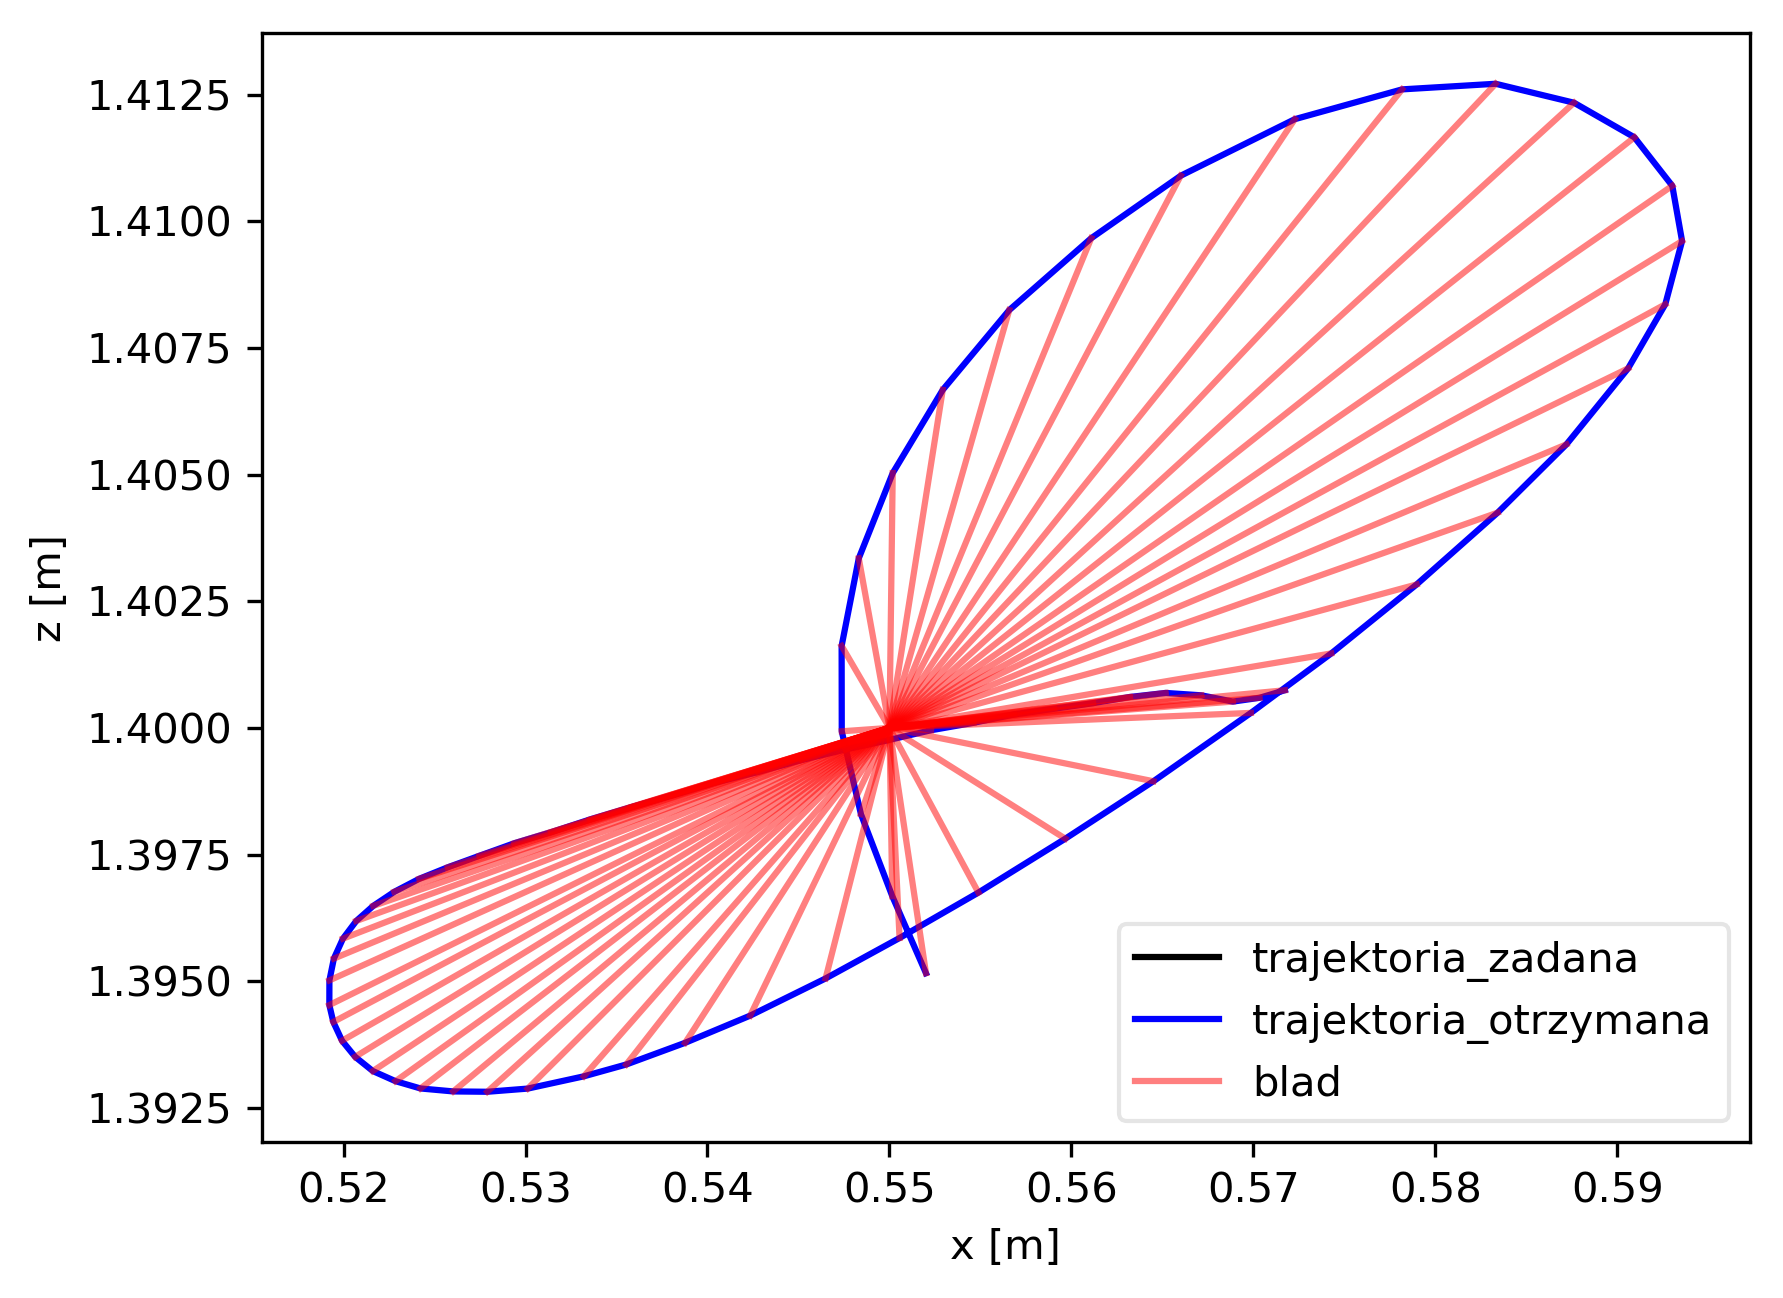
\includegraphics[width=.45\textwidth]{../../velma/przerobione_testy/out/w_bok_miekki/xz_ate_plot_podnoszenie_miekki_komp_piwo.png}
% 	}
% 	\hfill
% 	\subfigure[Trajektoria z chwycona wiertarka]{
% 		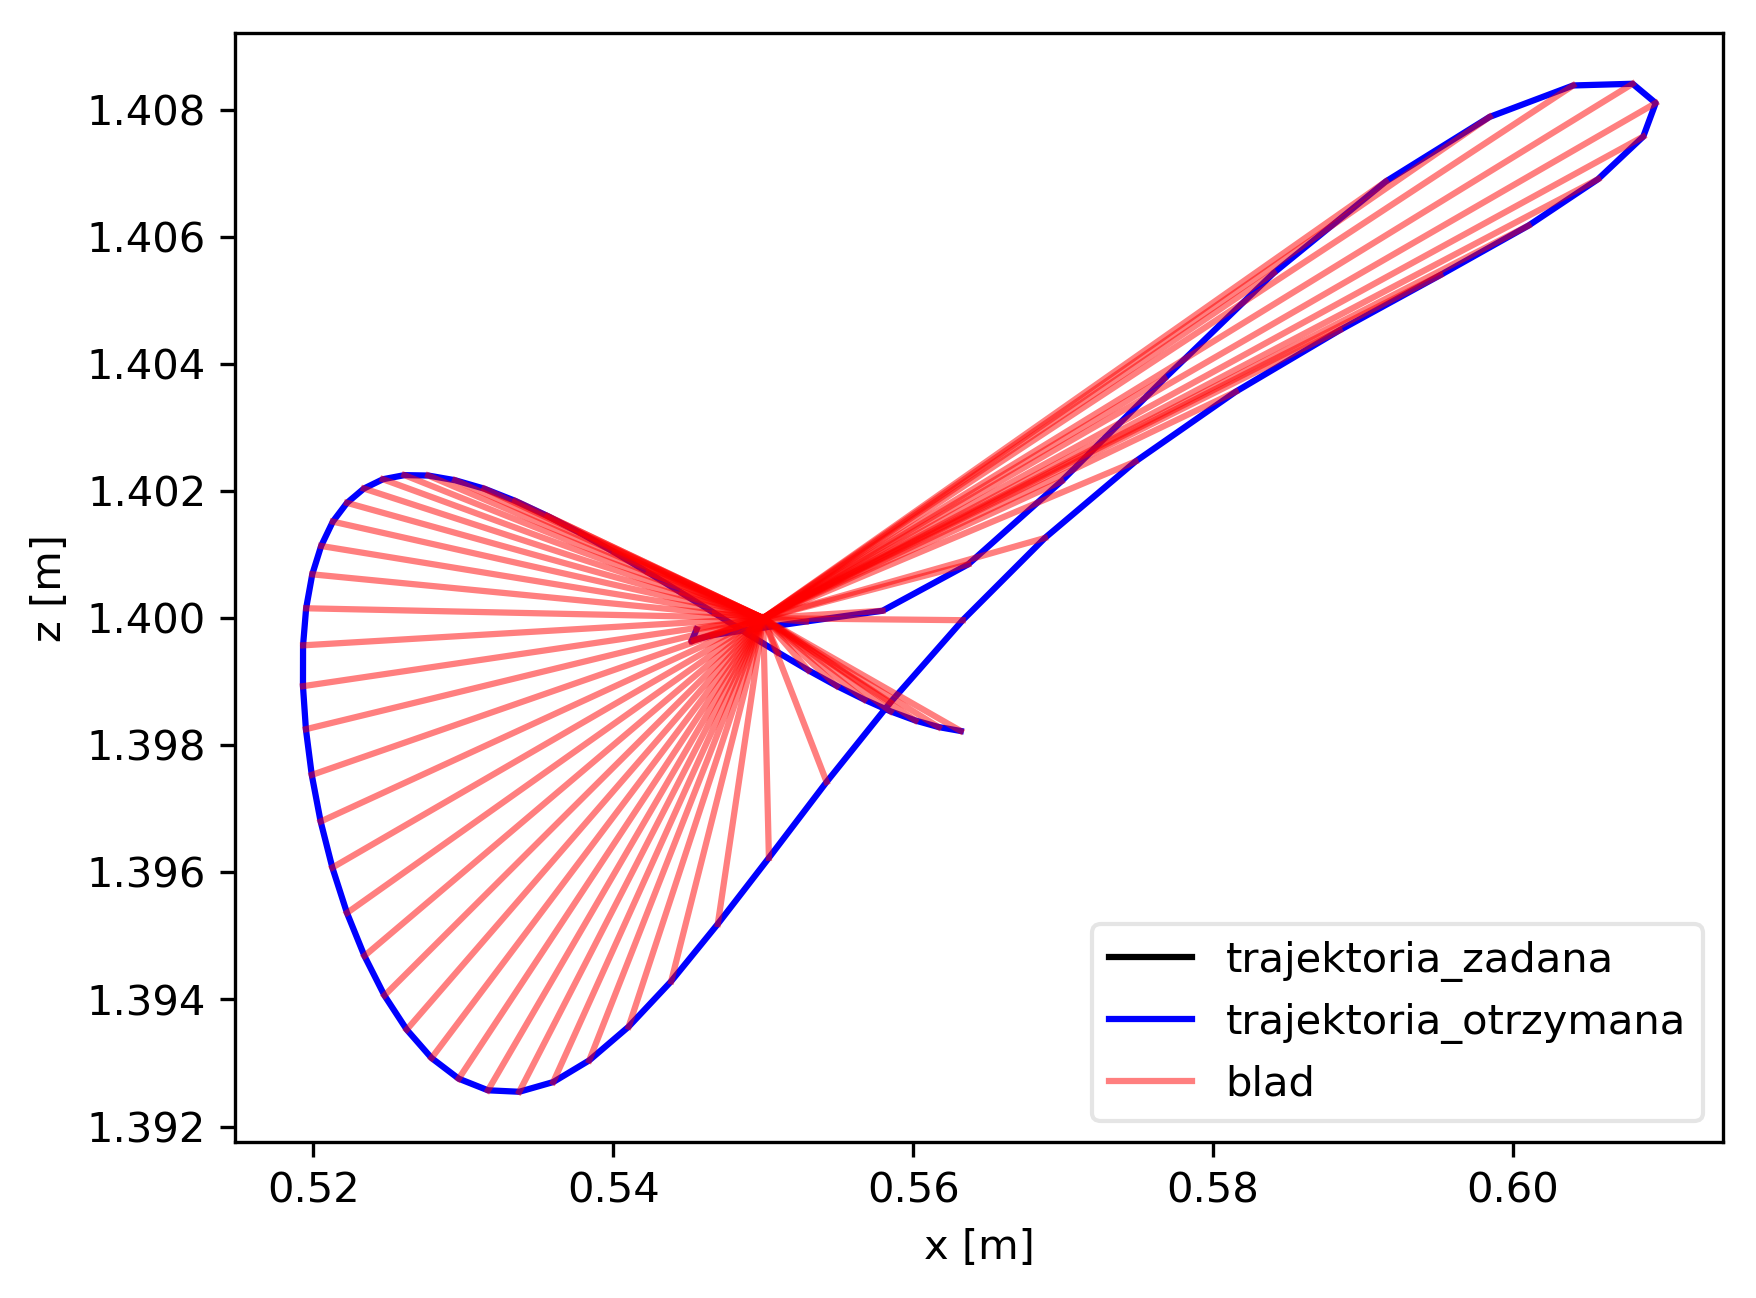
\includegraphics[width=.45\textwidth]{../../velma/przerobione_testy/out/w_bok_miekki/xz_ate_plot_podnoszenie_miekki_komp_wiertarka.png}
% 	}
% 	\caption{Porownanie trajektorii chwytaka w osiach $X$ i $Z$}
% 	\label{fig:w_bok_miekki_porow_przedm_bok}
% \end{figure}

\begin{figure}[h]
	\centering
	\subfigure[Rzut na wprost]{
		\label{fig:w_bok_miekki_porow_zbiorcze_a}
		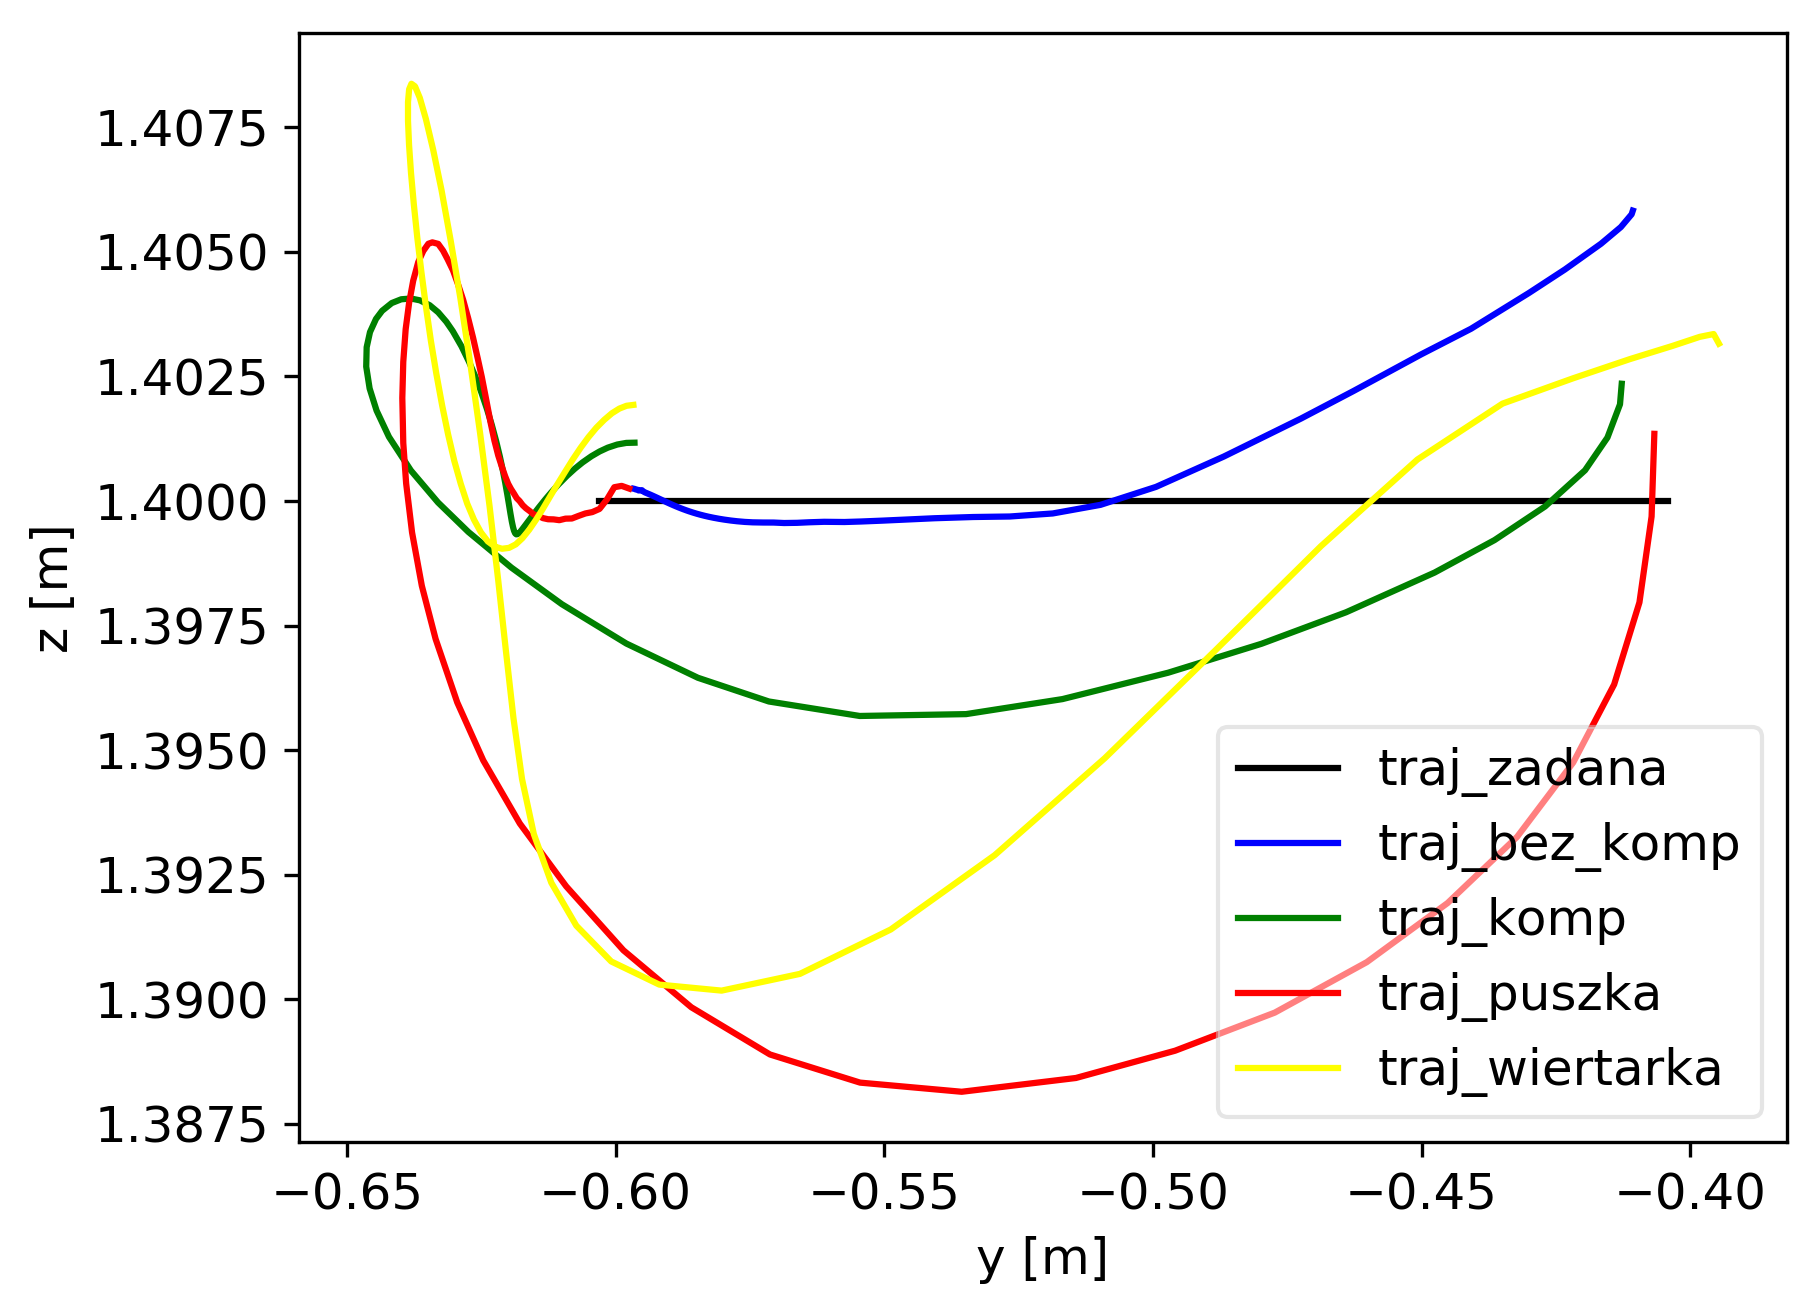
\includegraphics[width=.45\textwidth]{../../velma/przerobione_testy/out/w_bok_miekki/common_yz.png}
	}
	\hfill
	% \subfigure[Rzut z boku]{
	% 	\label{fig:w_bok_miekki_porow_zbiorcze_b}
	% 	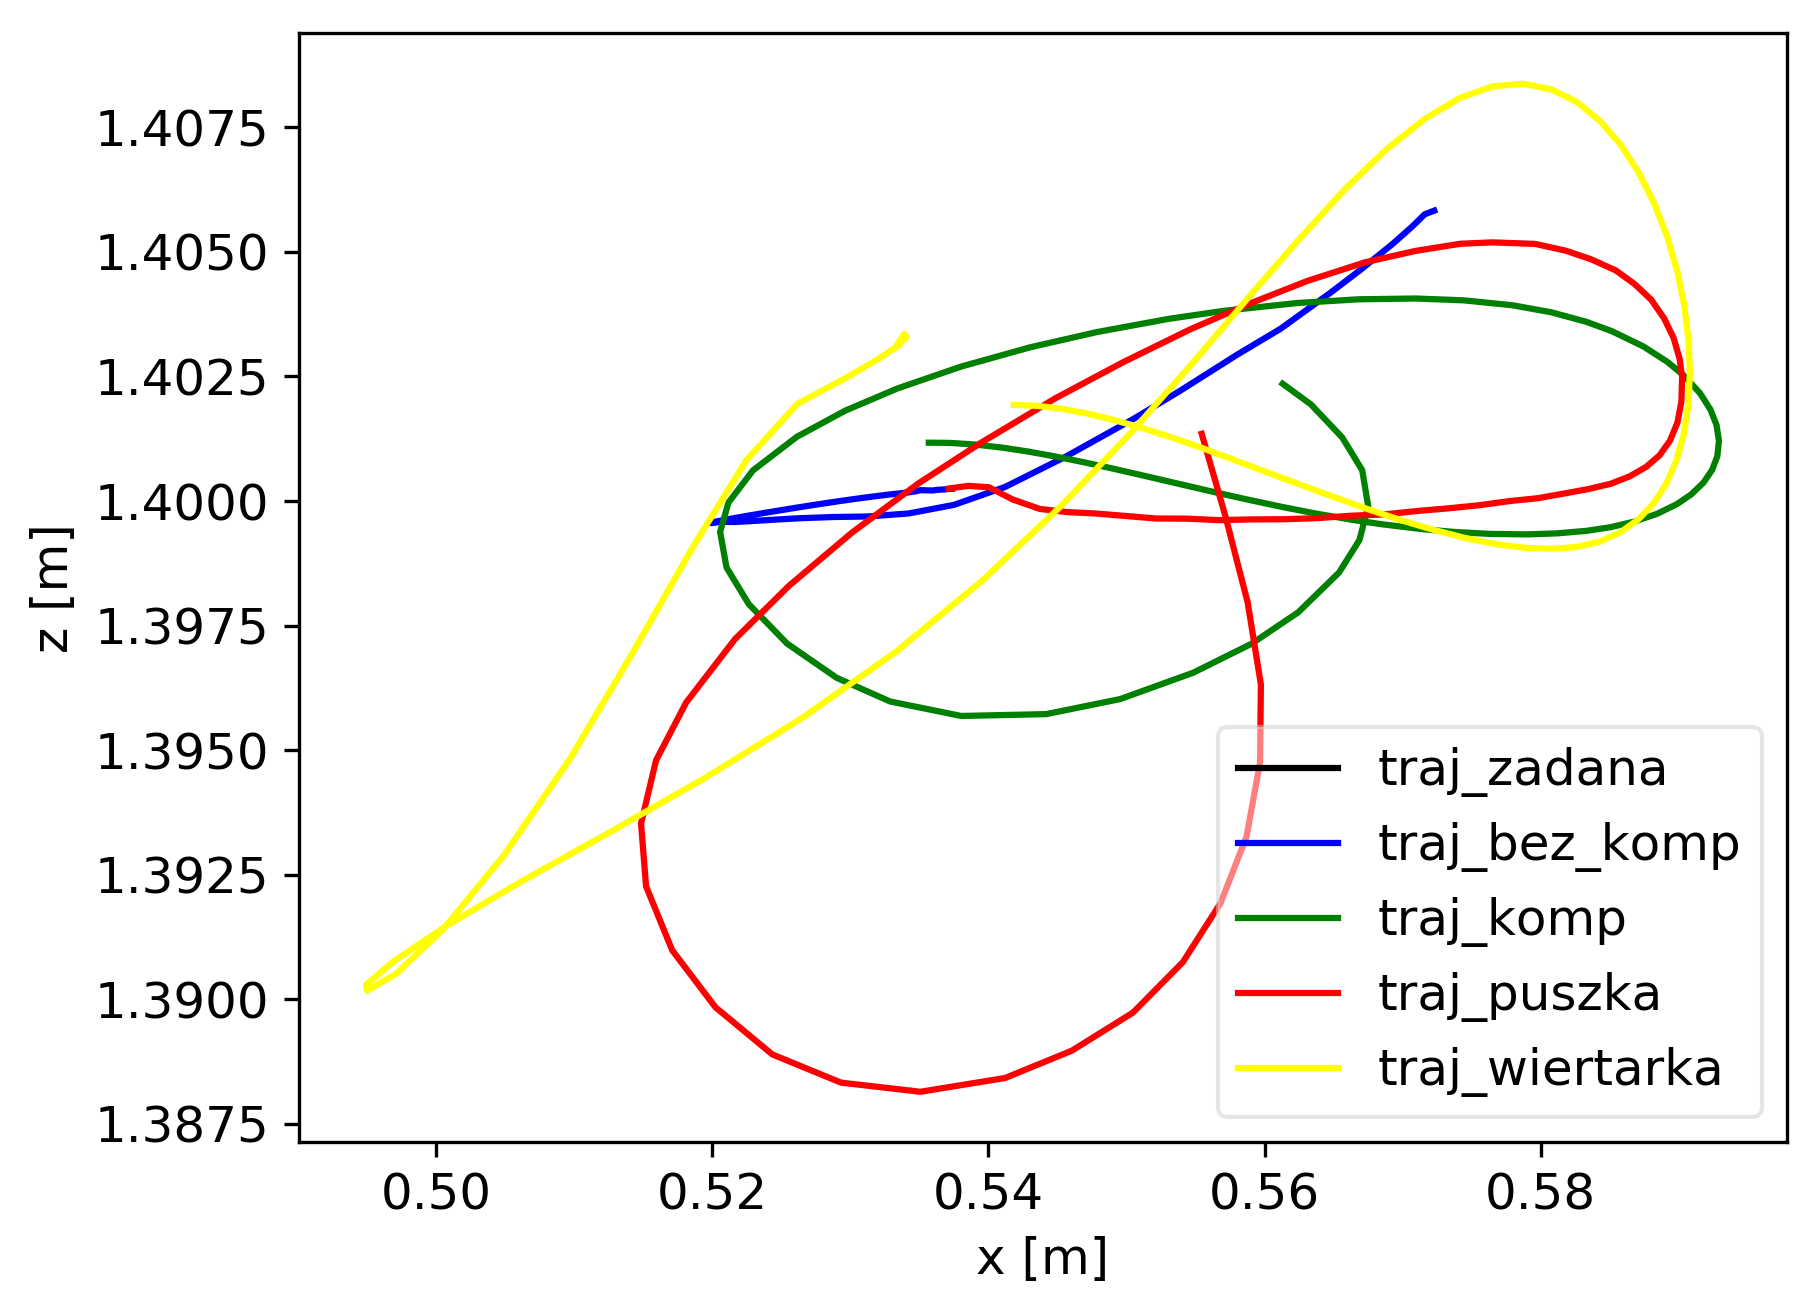
\includegraphics[width=.45\textwidth]{../../velma/przerobione_testy/out/w_bok_miekki/common_xz.png}
	% }
	\caption{Porowanie wszystkich trajektorii.}
	\label{fig:w_bok_miekki_porow_zbiorcze}
\end{figure}


\subsection{Ruch do gory}

Eksperyment ma przetestowac zachowanie algorytmu kompensacji przy ruchu koncowki do gory (rys. \ref{fig:do_gory_a}, \ref{fig:do_gory_rot}). Jest to dla algorytmu potencjalnie trudny ruch z przez sile grawitacji dzialajaca wlasnie w tej osi. Trajektoria ruchu w rzucie APE zostala zaprezentowana na rys. \ref{fig:do_gory_porow_komp}, \ref{fig:do_gory_porow_przedm} i \ref{fig:do_gory_porow_zbiorcze_a}.

\begin{figure}[h]
	\centering
	\subfigure[Os $X$]{
		\label{fig:do_gory_ax}
		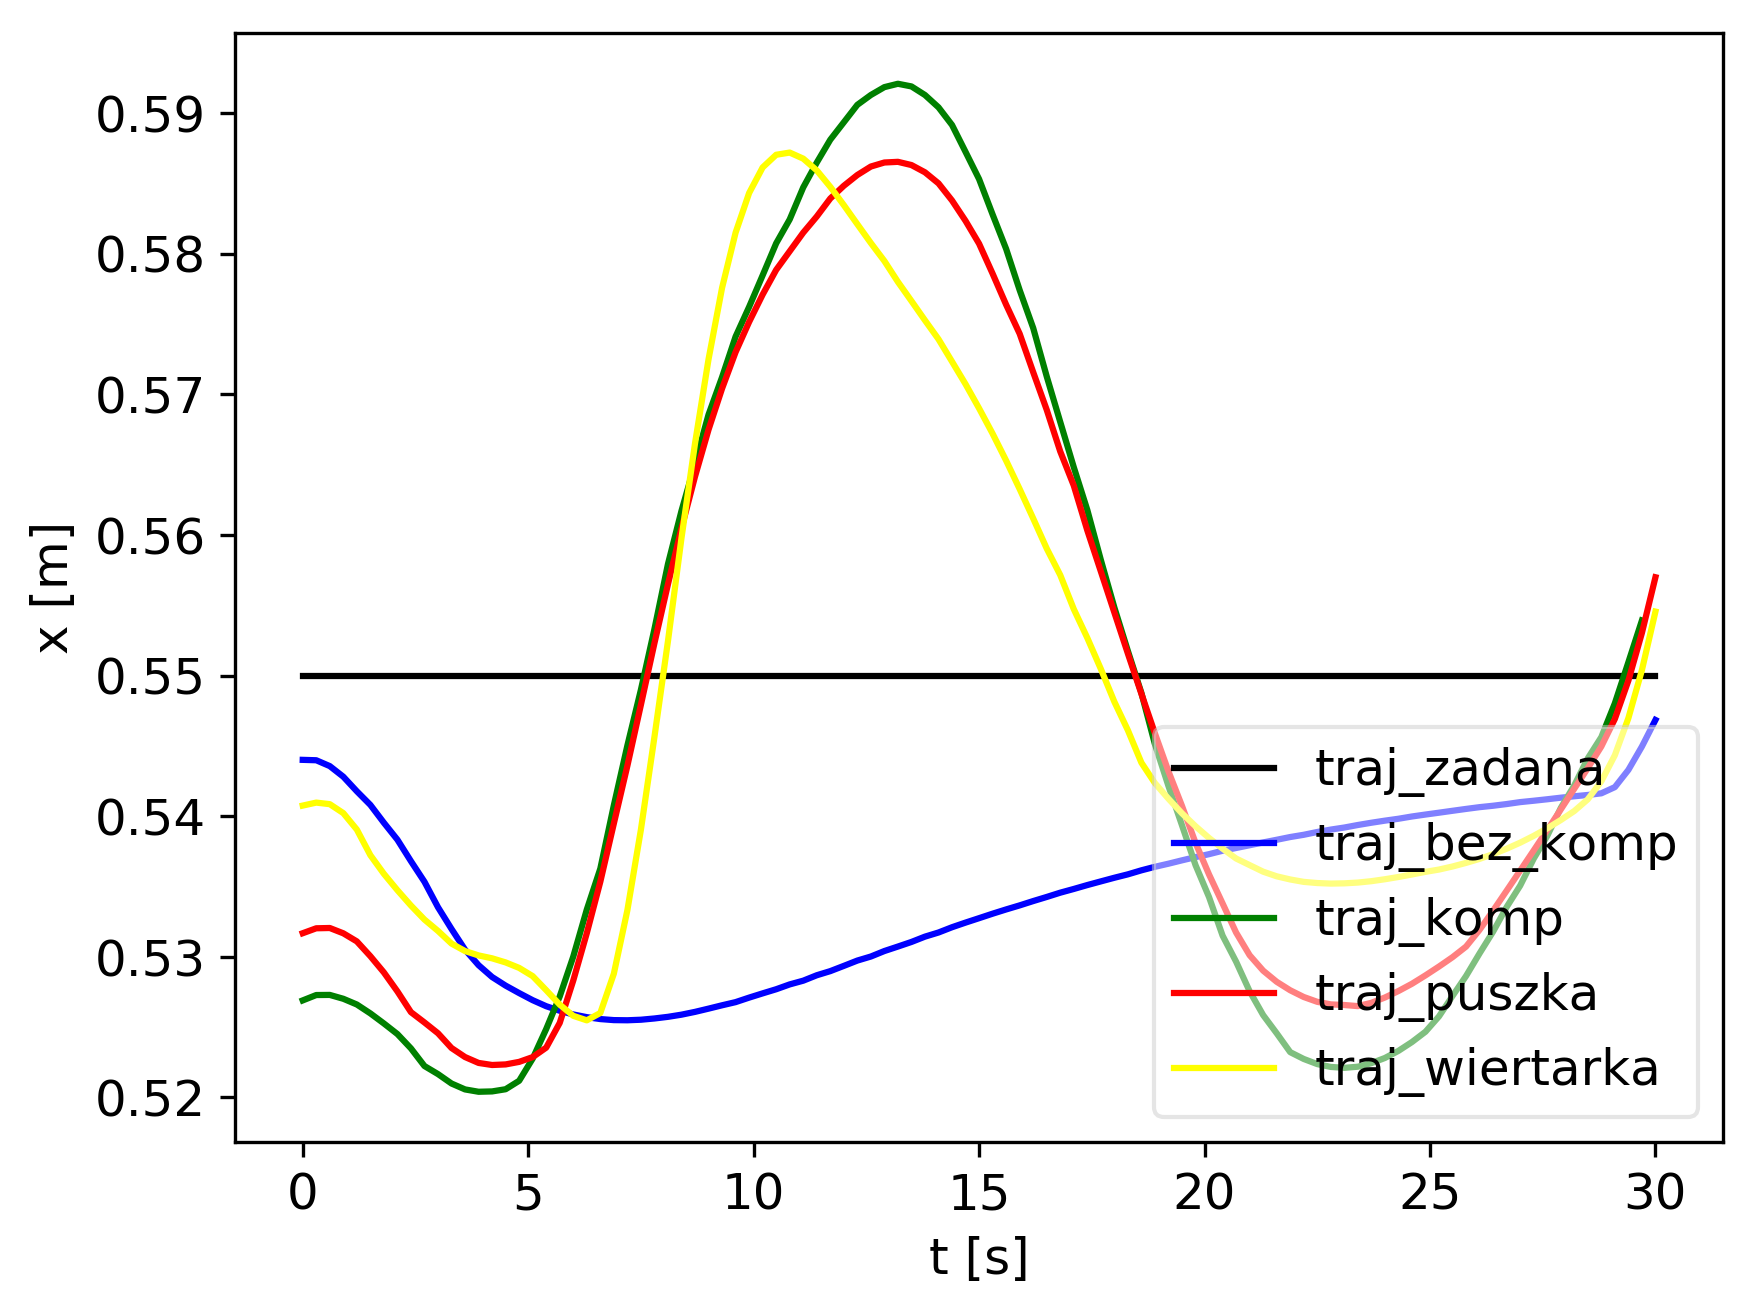
\includegraphics[width=.45\textwidth]{../../velma/przerobione_testy/out/do_gory/common_ax.png}
	}
	\hfill
	\subfigure[Os $Y$]{
		\label{fig:do_gory_ay}
		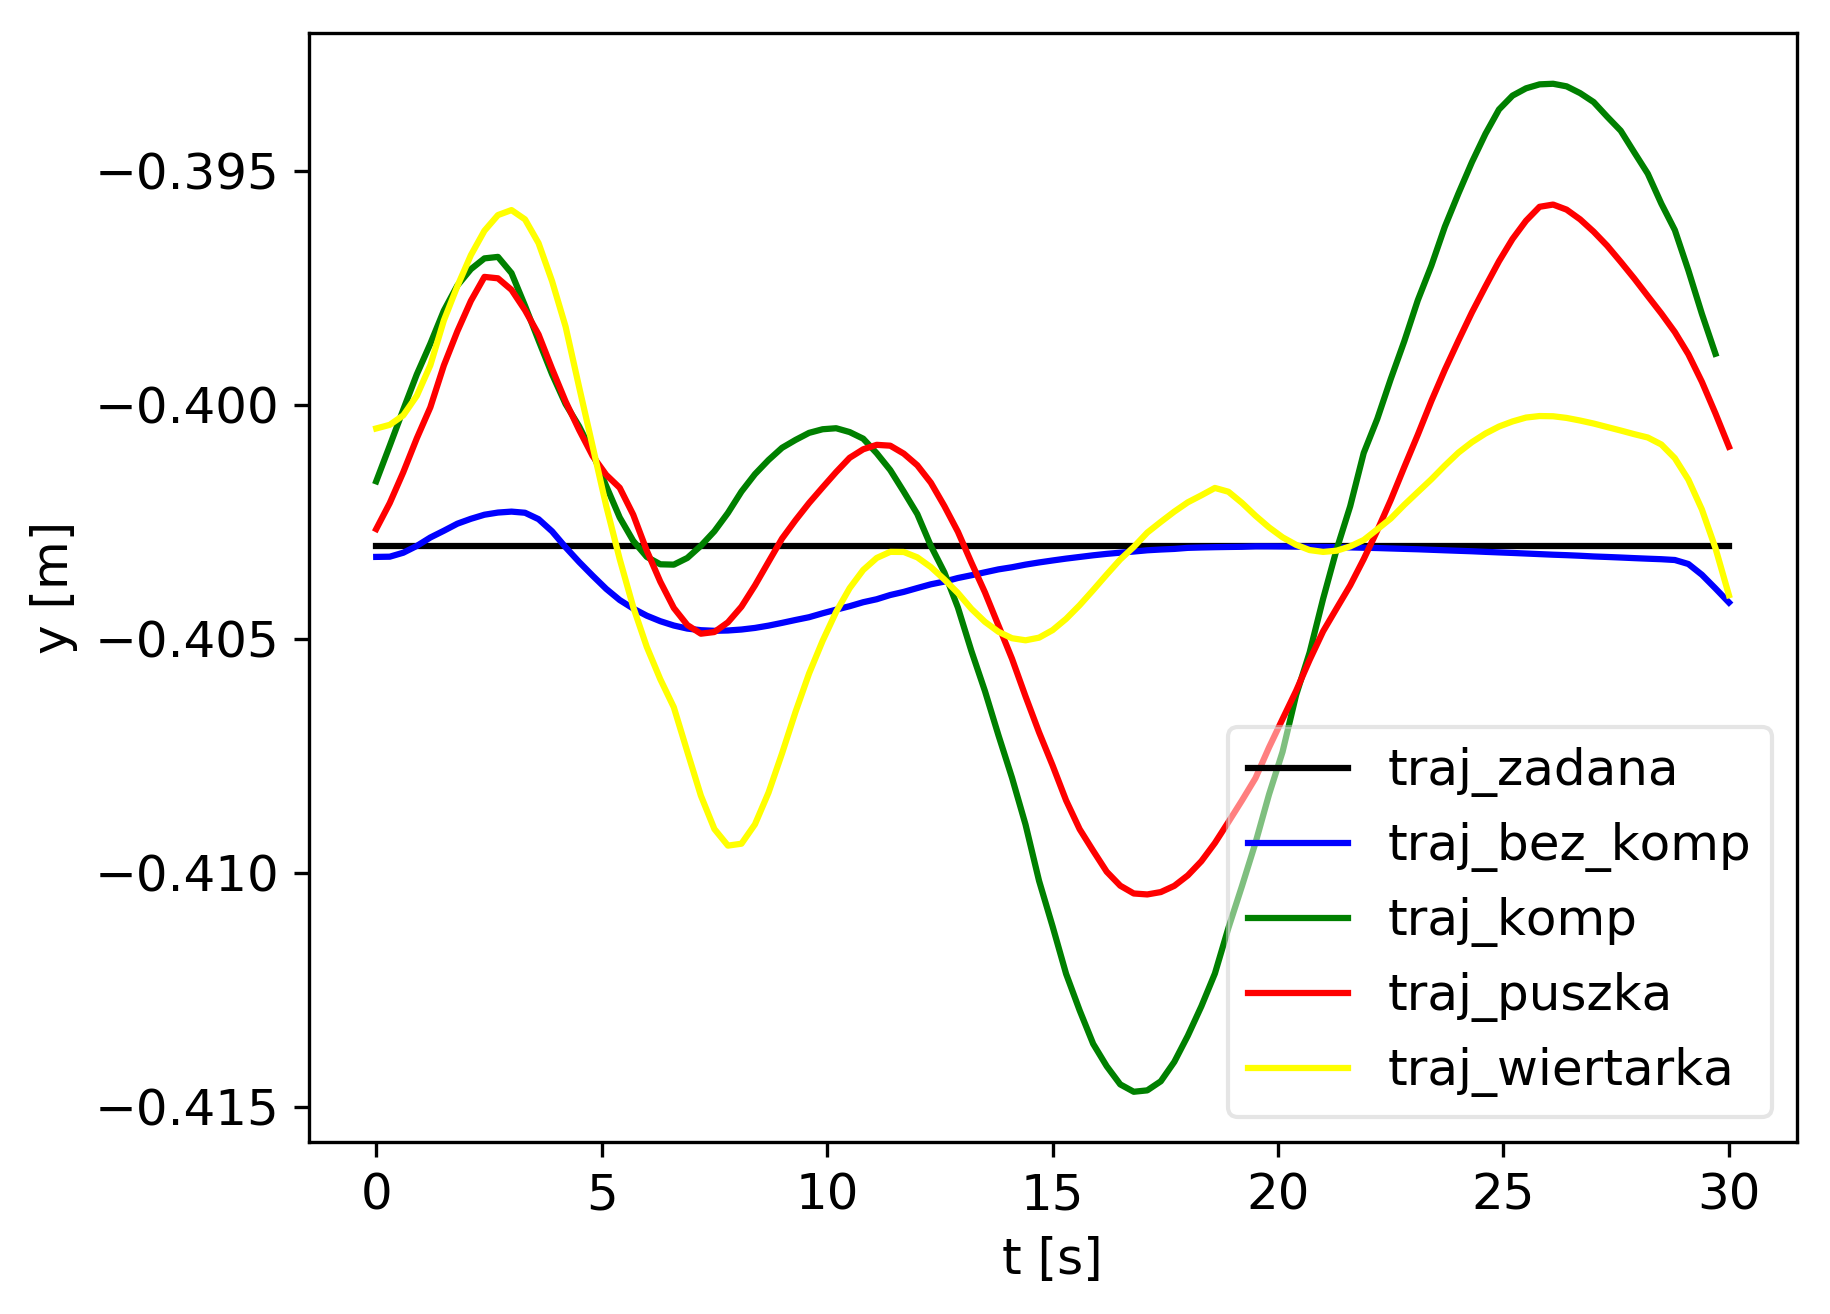
\includegraphics[width=.45\textwidth]{../../velma/przerobione_testy/out/do_gory/common_ay.png}
	}
	
	\hfill
	\subfigure[Os $Z$]{
		\label{fig:do_gory_az}
		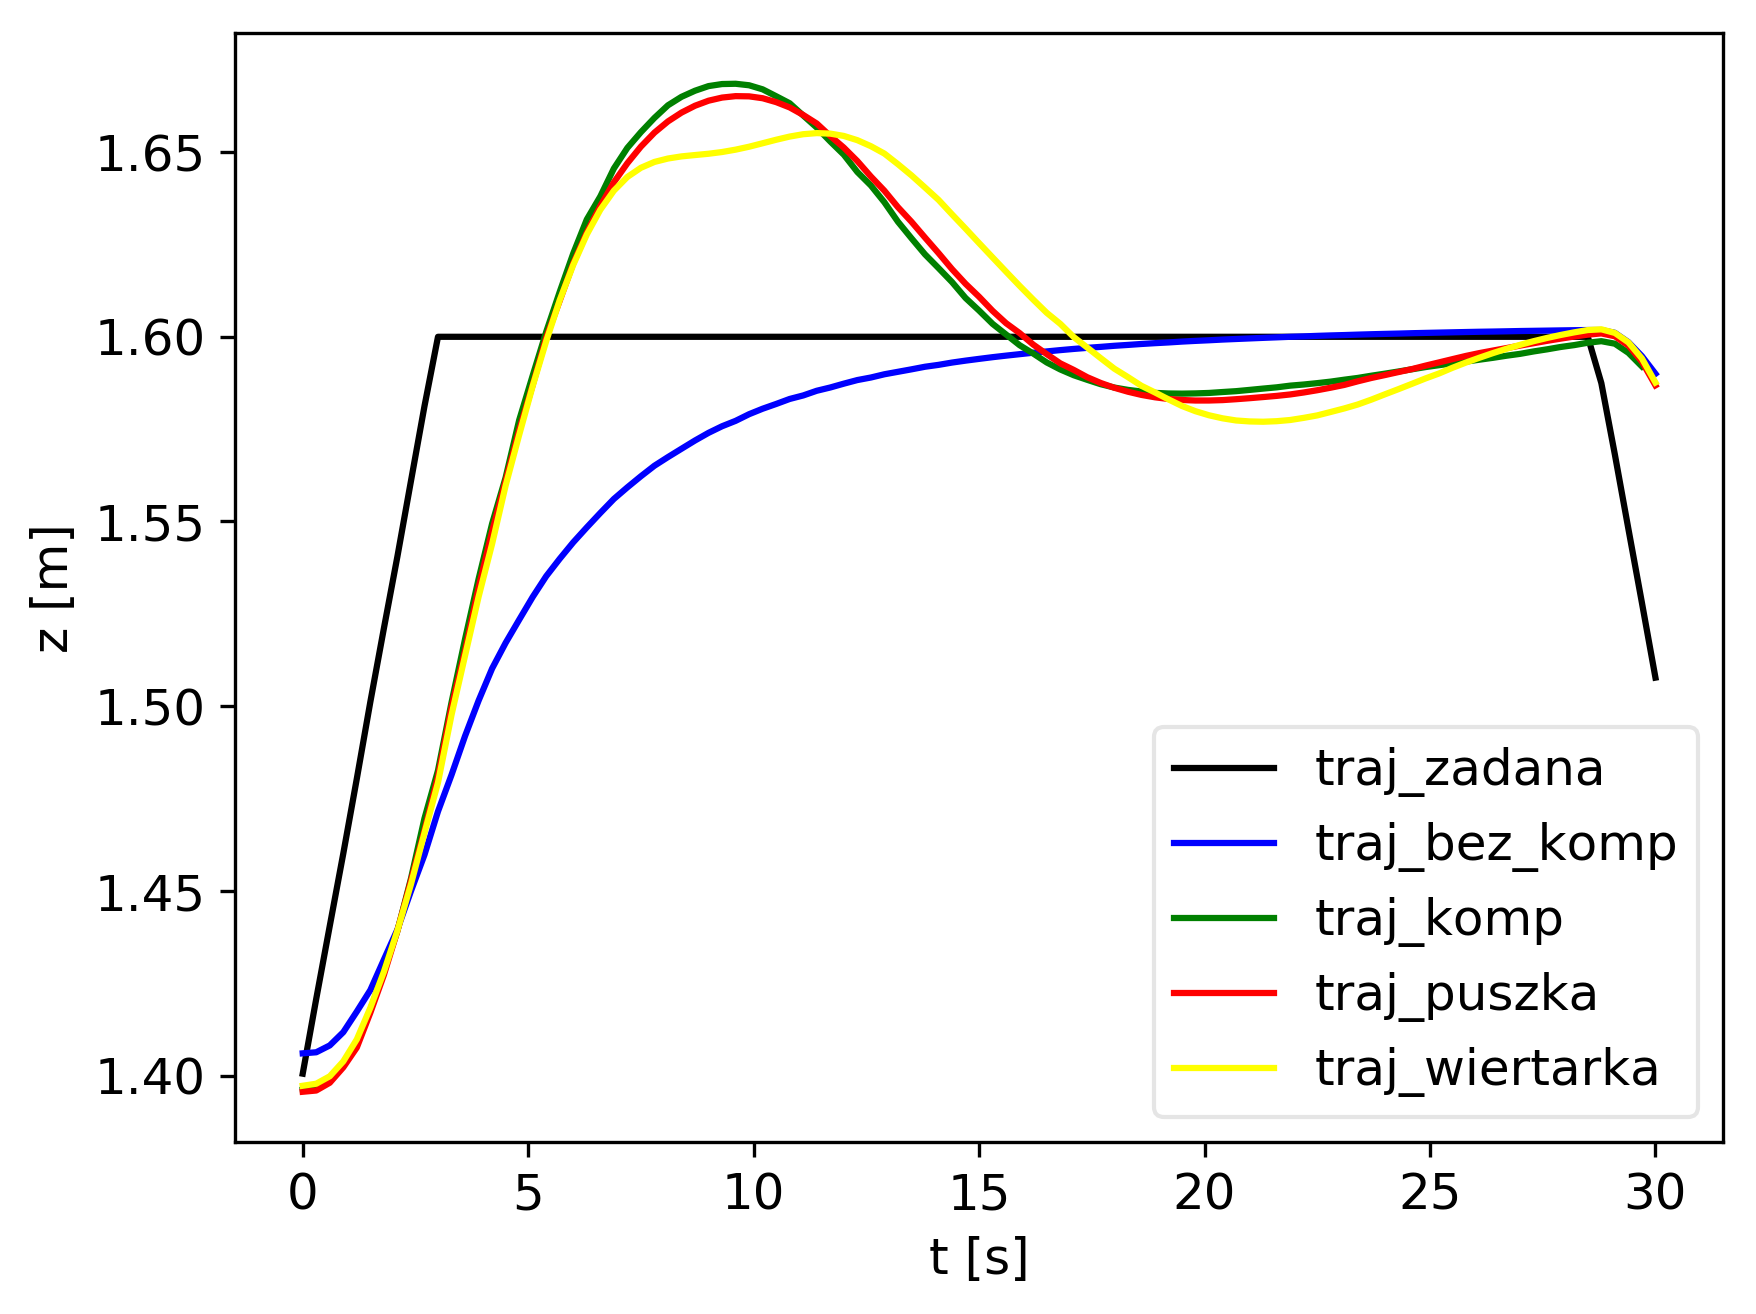
\includegraphics[width=.45\textwidth]{../../velma/przerobione_testy/out/do_gory/common_az.png}
	}

	\caption{Ruch do gory. Porownanie trajektorii pozycji w zaleznosci od czasu.}
	\label{fig:do_gory_a}

\end{figure}


\begin{figure}[h]
	\centering
	\subfigure[Kat osi $X$]{
		\label{fig:do_gory_rotx}
		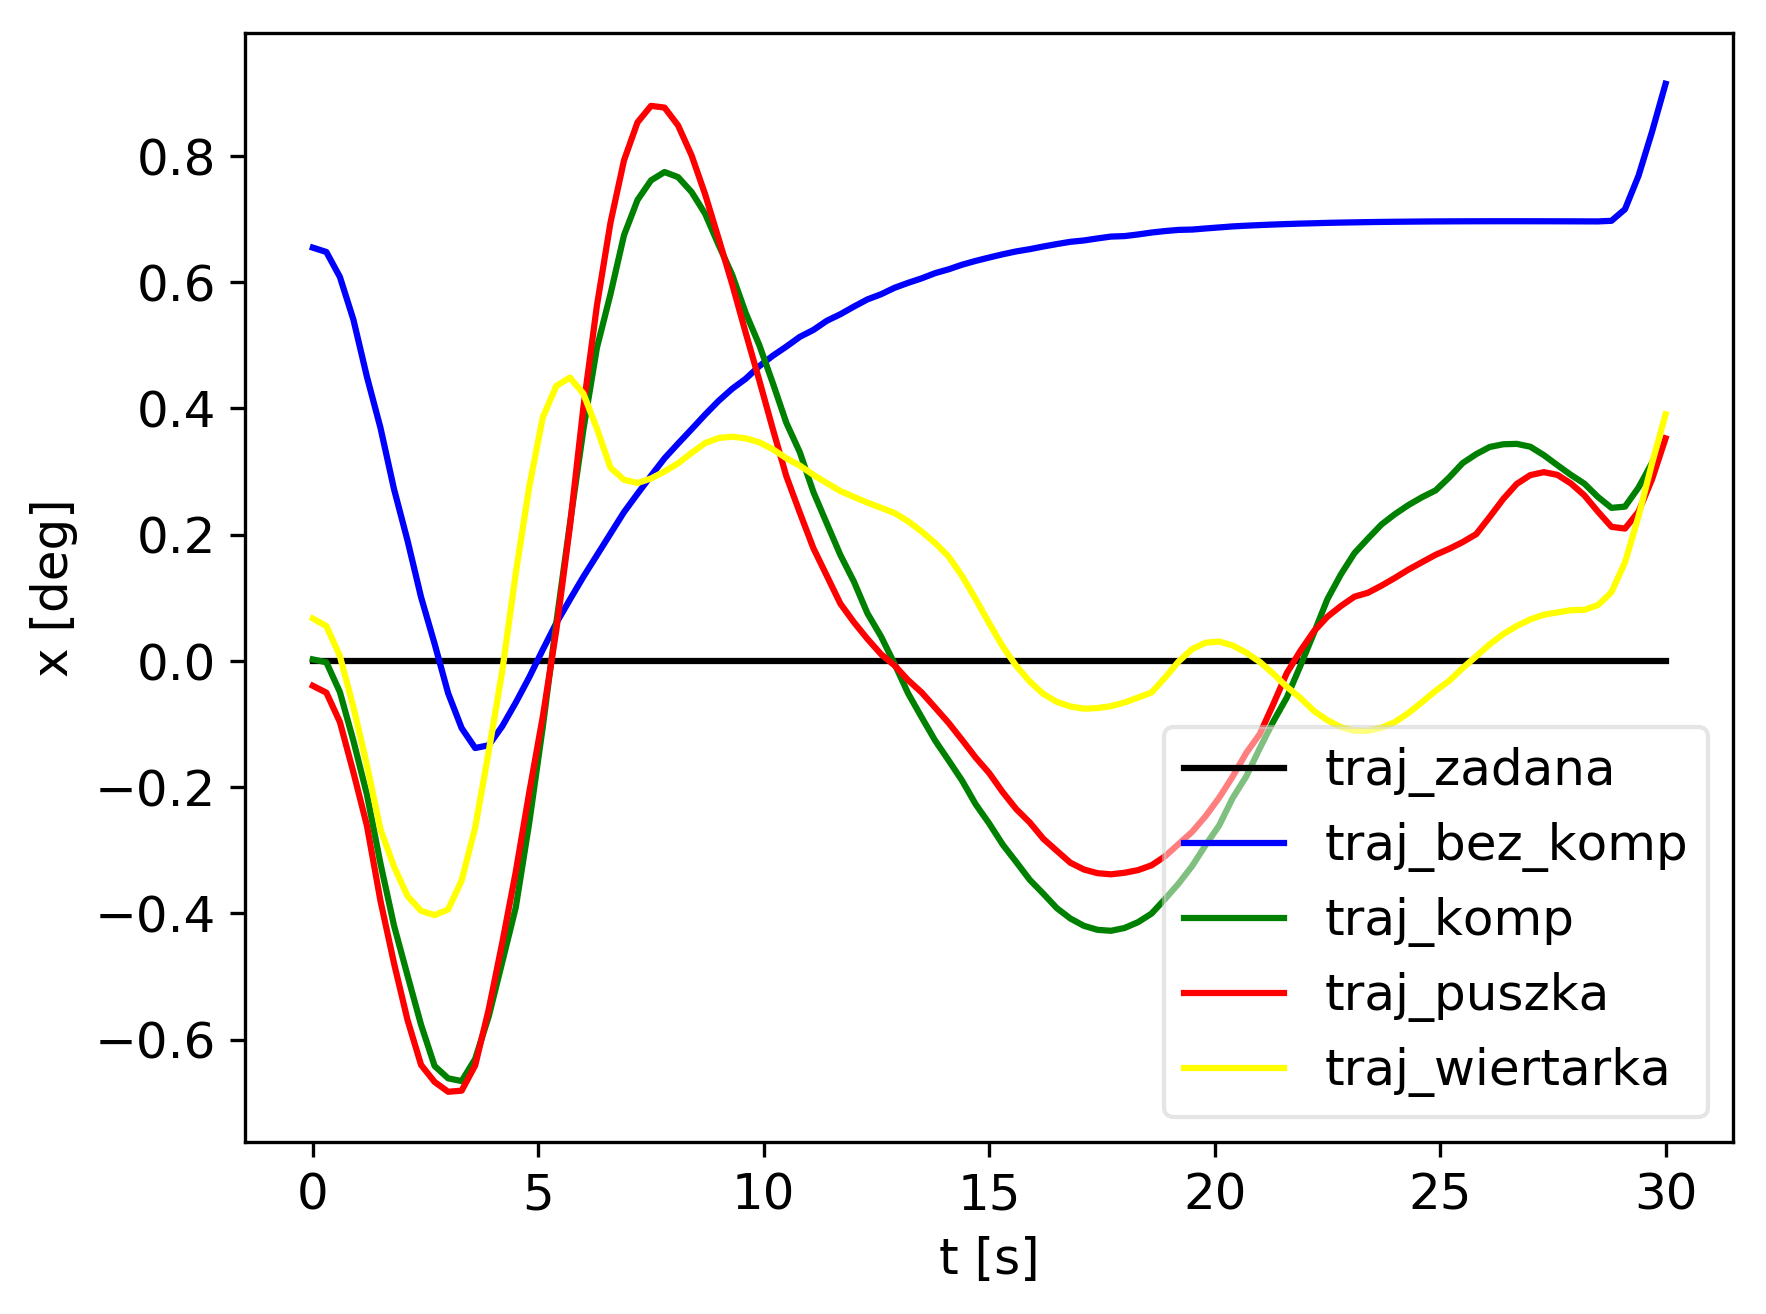
\includegraphics[width=.45\textwidth]{../../velma/przerobione_testy/out/do_gory/common_rotx.png}
	}
	\hfill
	\subfigure[Kat osi $Y$]{
		\label{fig:do_gory_roty}
		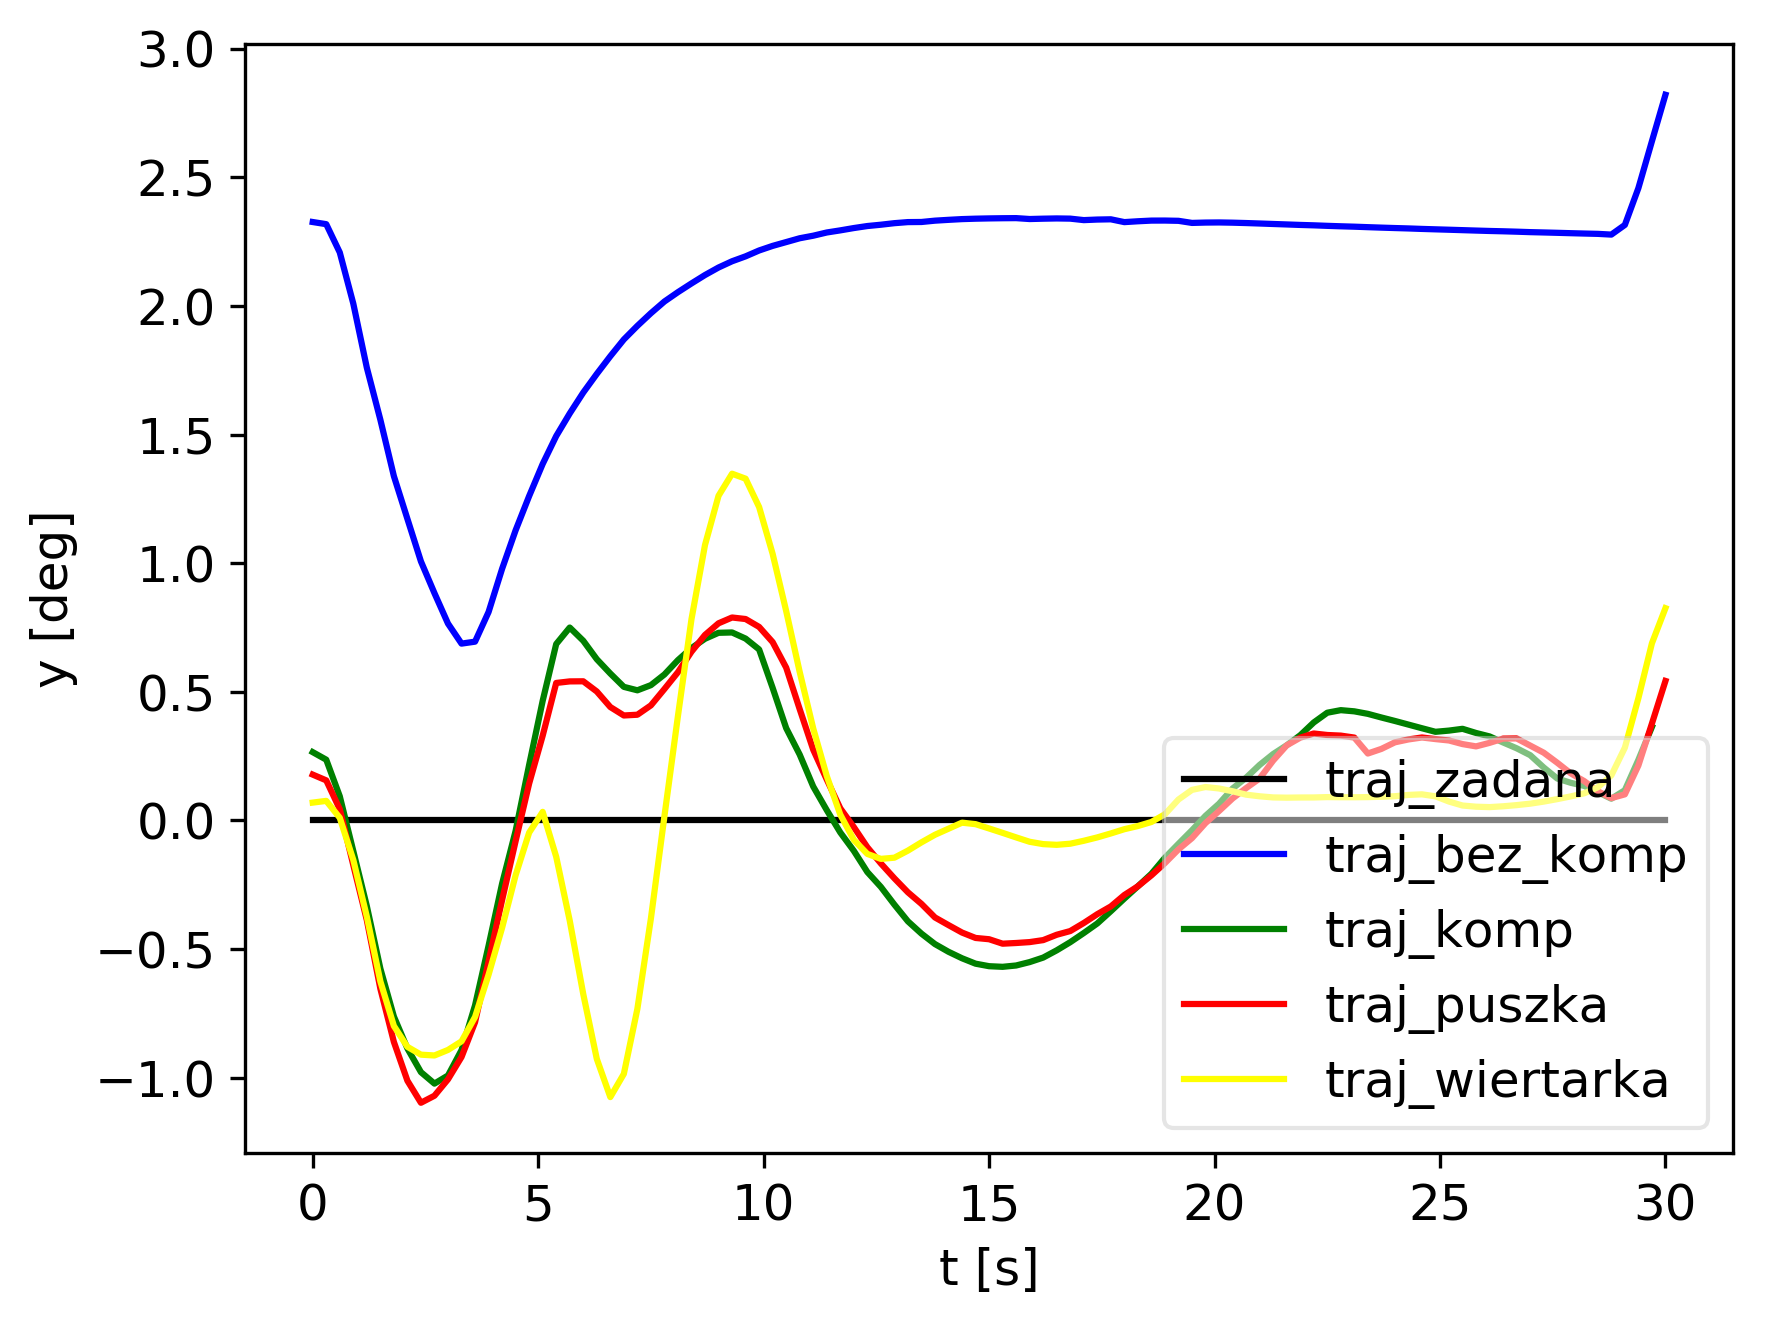
\includegraphics[width=.45\textwidth]{../../velma/przerobione_testy/out/do_gory/common_roty.png}
	}
	
	\hfill
	\subfigure[Kat osi $Z$]{
		\label{fig:do_gory_rotz}
		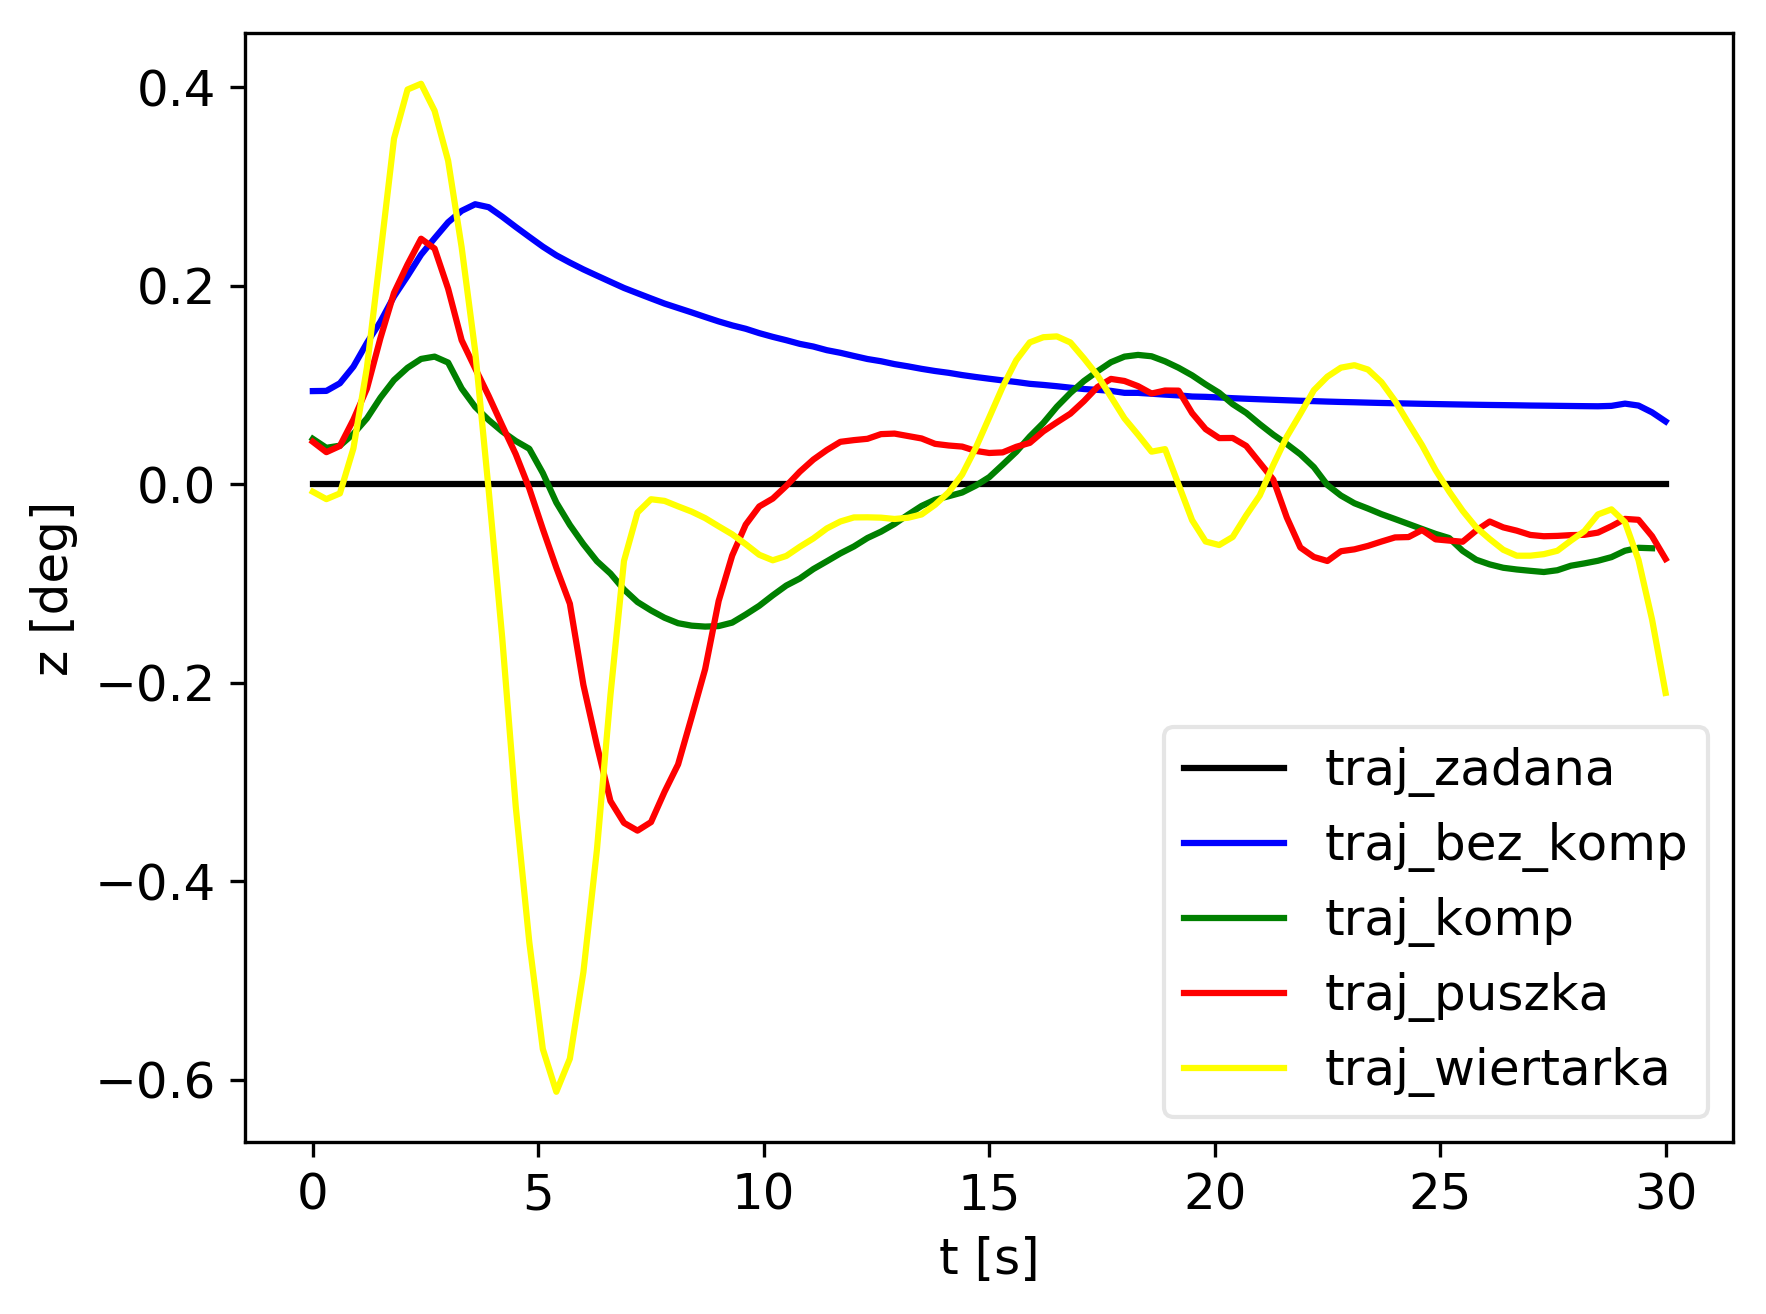
\includegraphics[width=.45\textwidth]{../../velma/przerobione_testy/out/do_gory/common_rotz.png}
	}

	\caption{Ruch do gory. Porownanie trajektorii katow w notacji Eulera w zaleznosci od czasu.}
	\label{fig:do_gory_rot}

\end{figure}


\begin{figure}[h]
	\centering
	\subfigure[Brak algorytmu kompensacji]{
		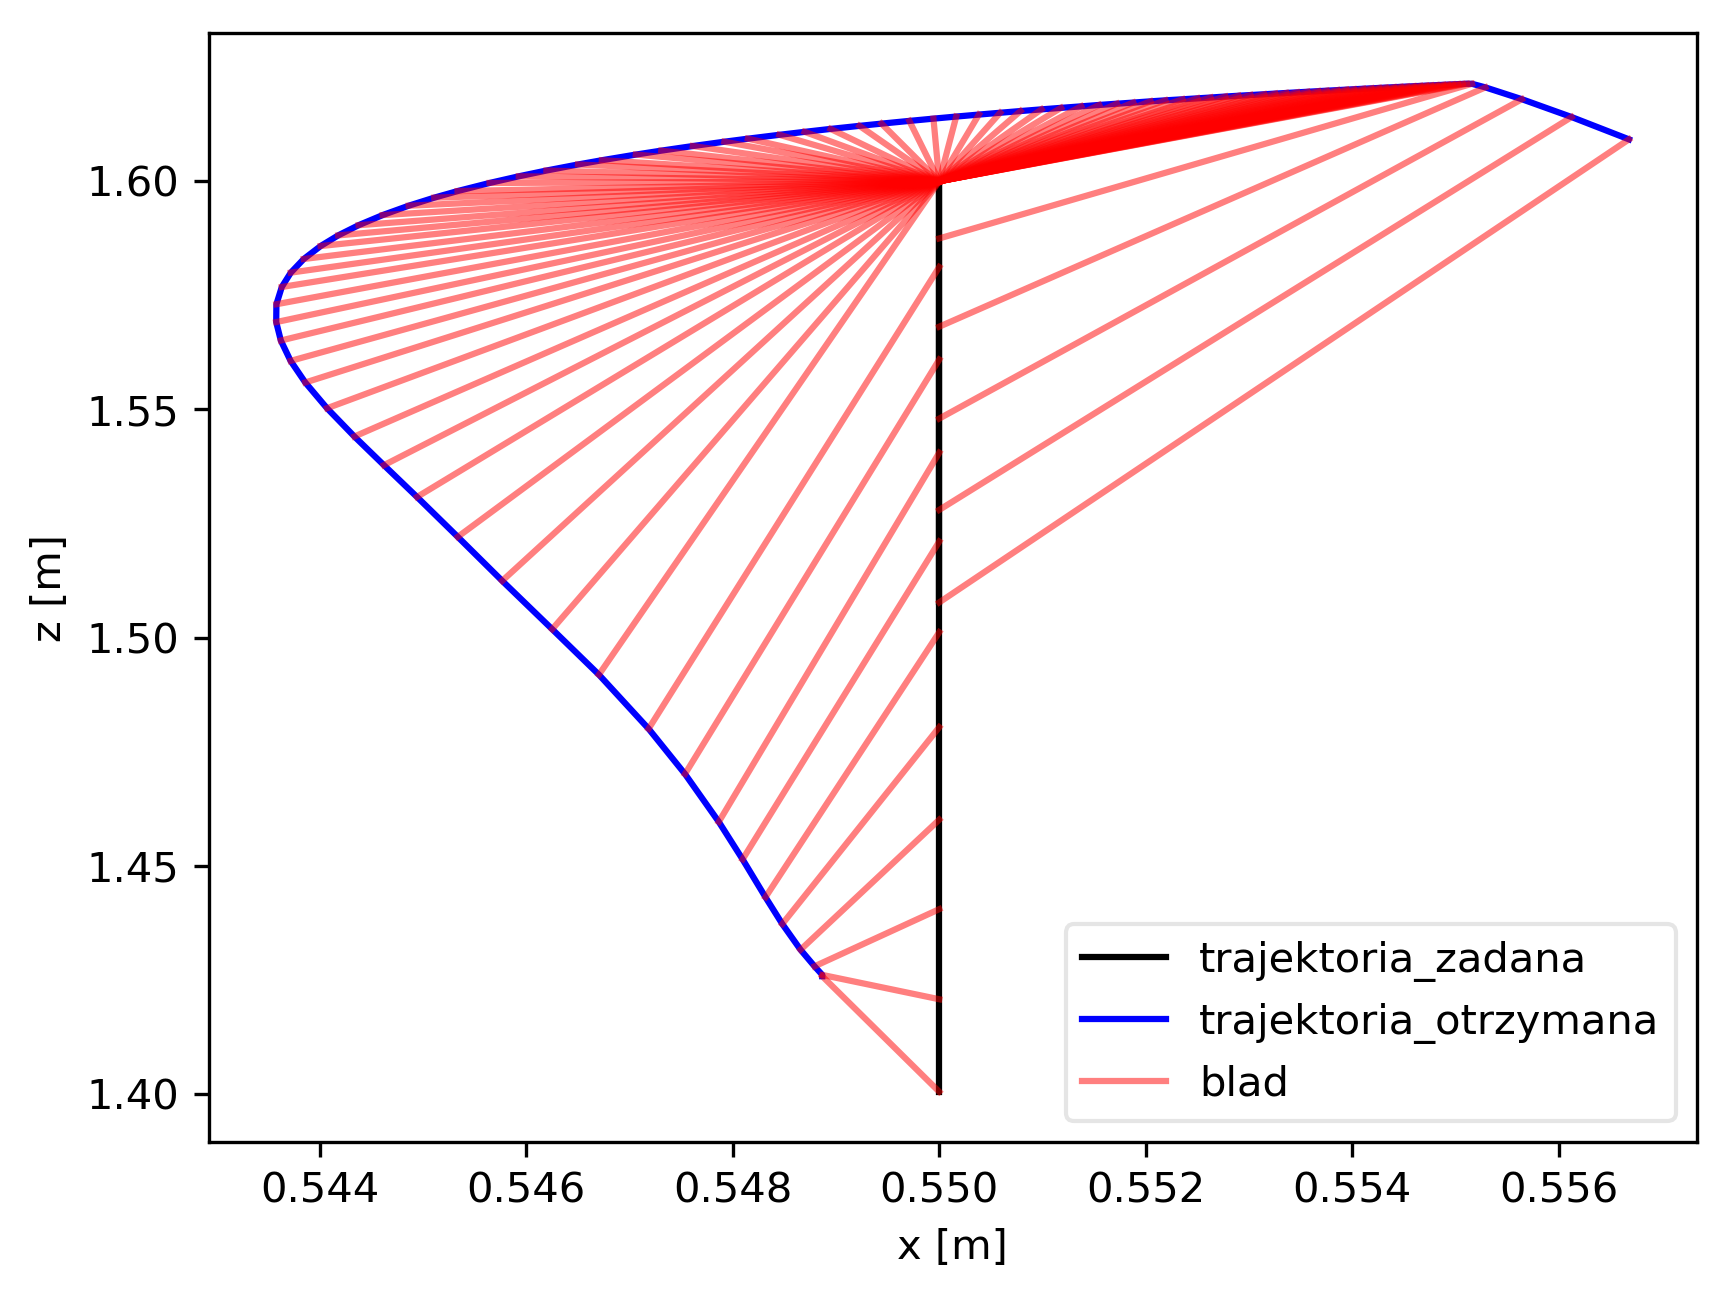
\includegraphics[width=.45\textwidth]{../../velma/przerobione_testy/out/do_gory/xz_ate_plot_podnoszenie_miekki_bez_brak.png}
	}
	\hfill
	\subfigure[Zalaczony algorytm kompnesacji]{
		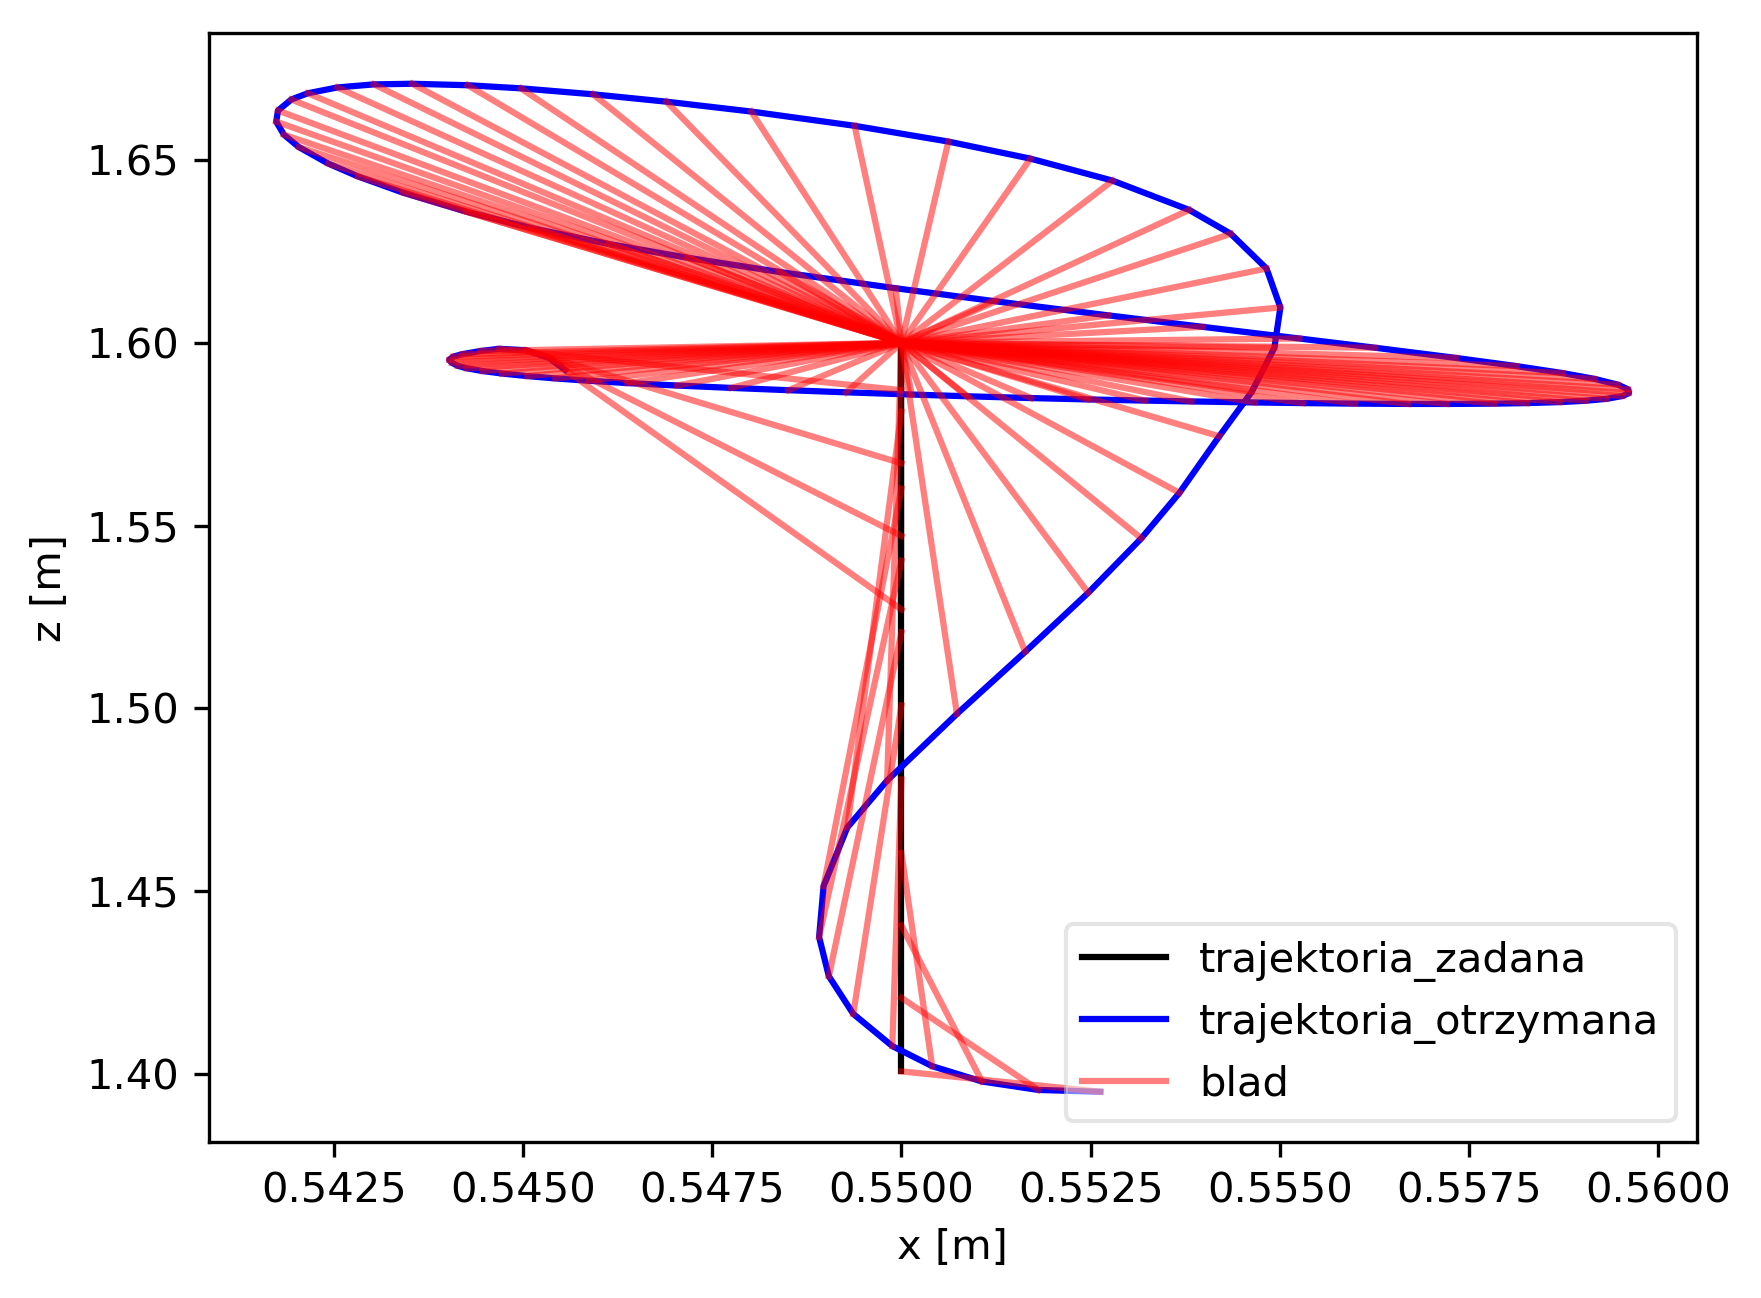
\includegraphics[width=.45\textwidth]{../../velma/przerobione_testy/out/do_gory/xz_ate_plot_podnoszenie_miekki_komp_brak.png}
	}
	\caption{Porownanie trajektorii chwytaka w osiach $X$ i $Z$}
	\label{fig:do_gory_porow_komp}
\end{figure}

\begin{figure}[h]
	\centering
	\subfigure[Trajektoria z chwycona puszka]{
		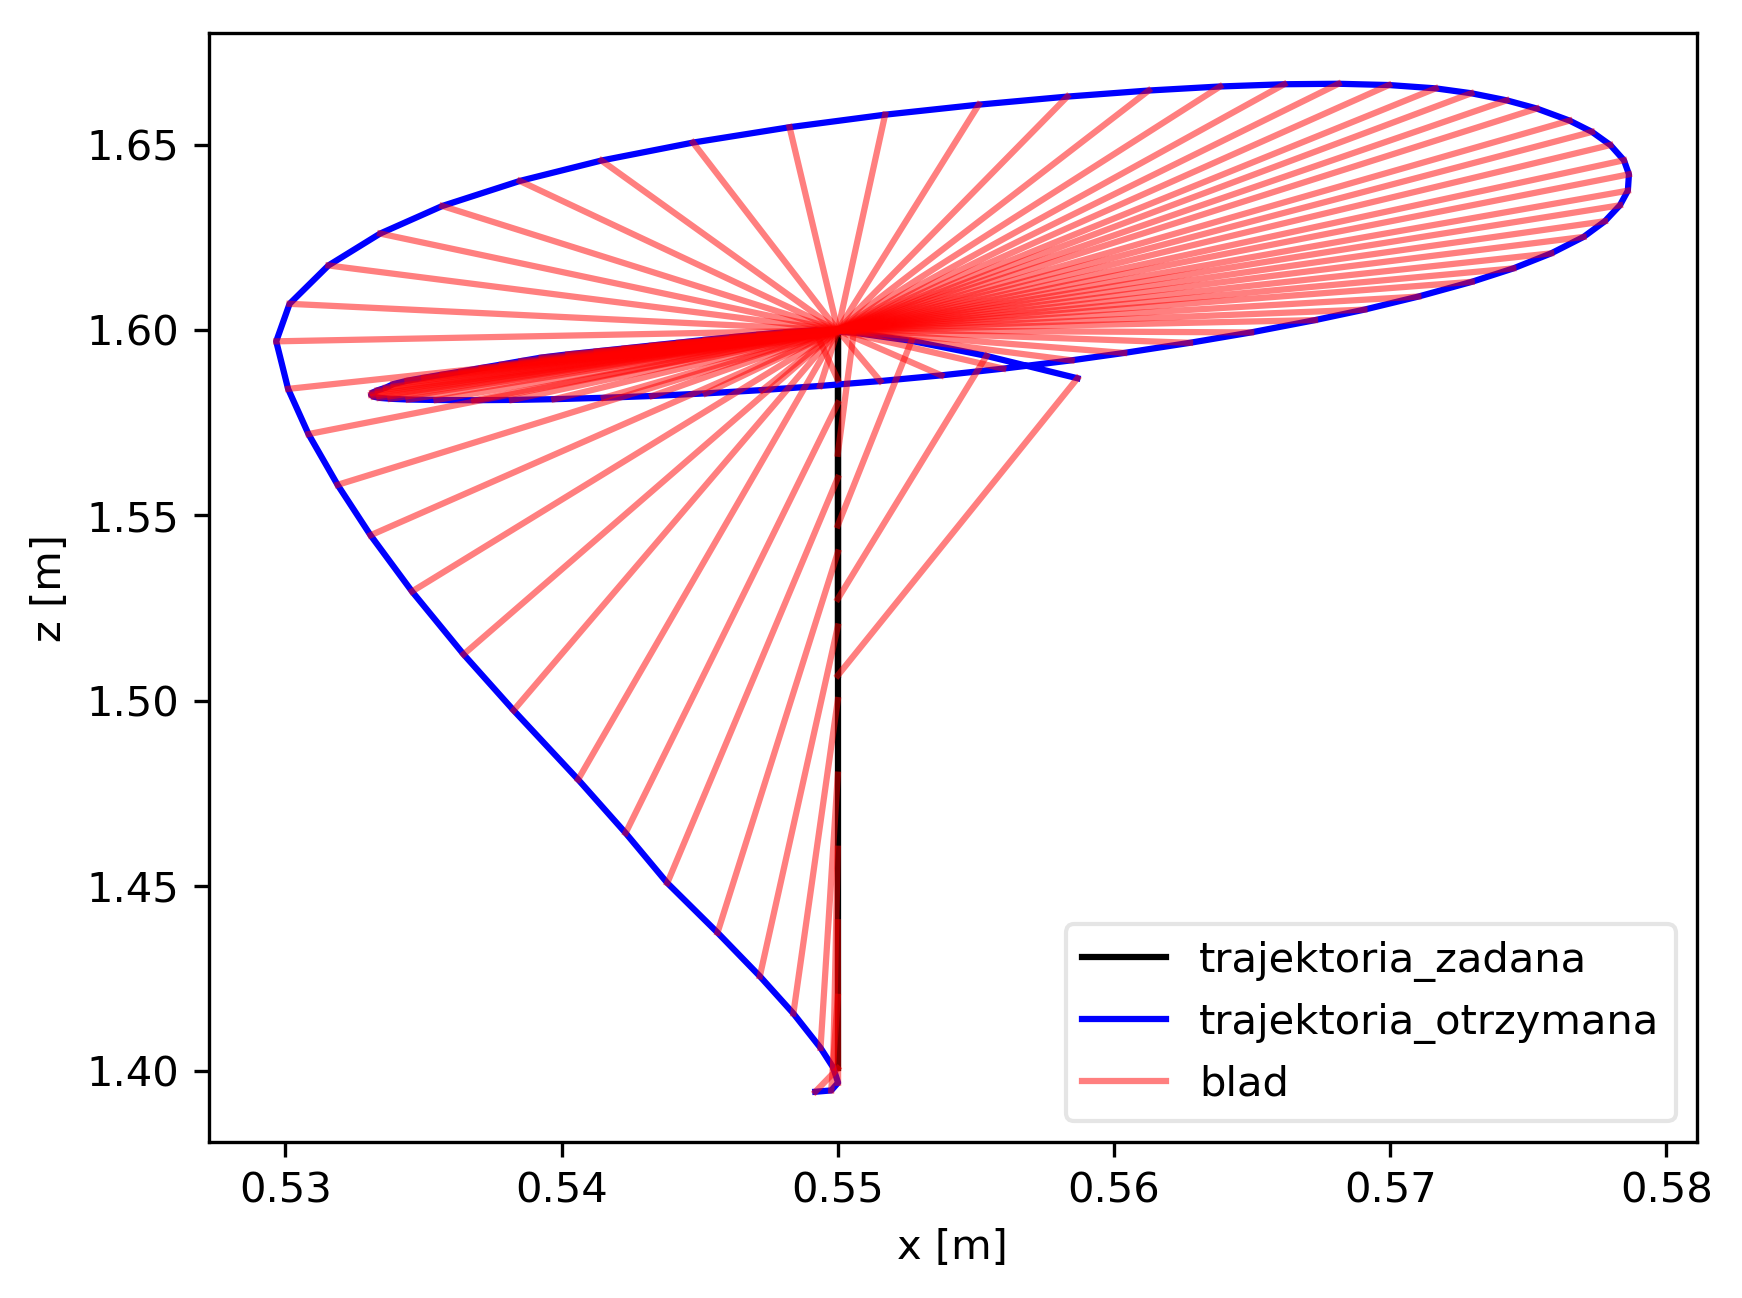
\includegraphics[width=.45\textwidth]{../../velma/przerobione_testy/out/do_gory/xz_ate_plot_podnoszenie_miekki_komp_piwo.png}
	}
	\hfill
	\subfigure[Trajektoria z chwycona wiertarka]{
		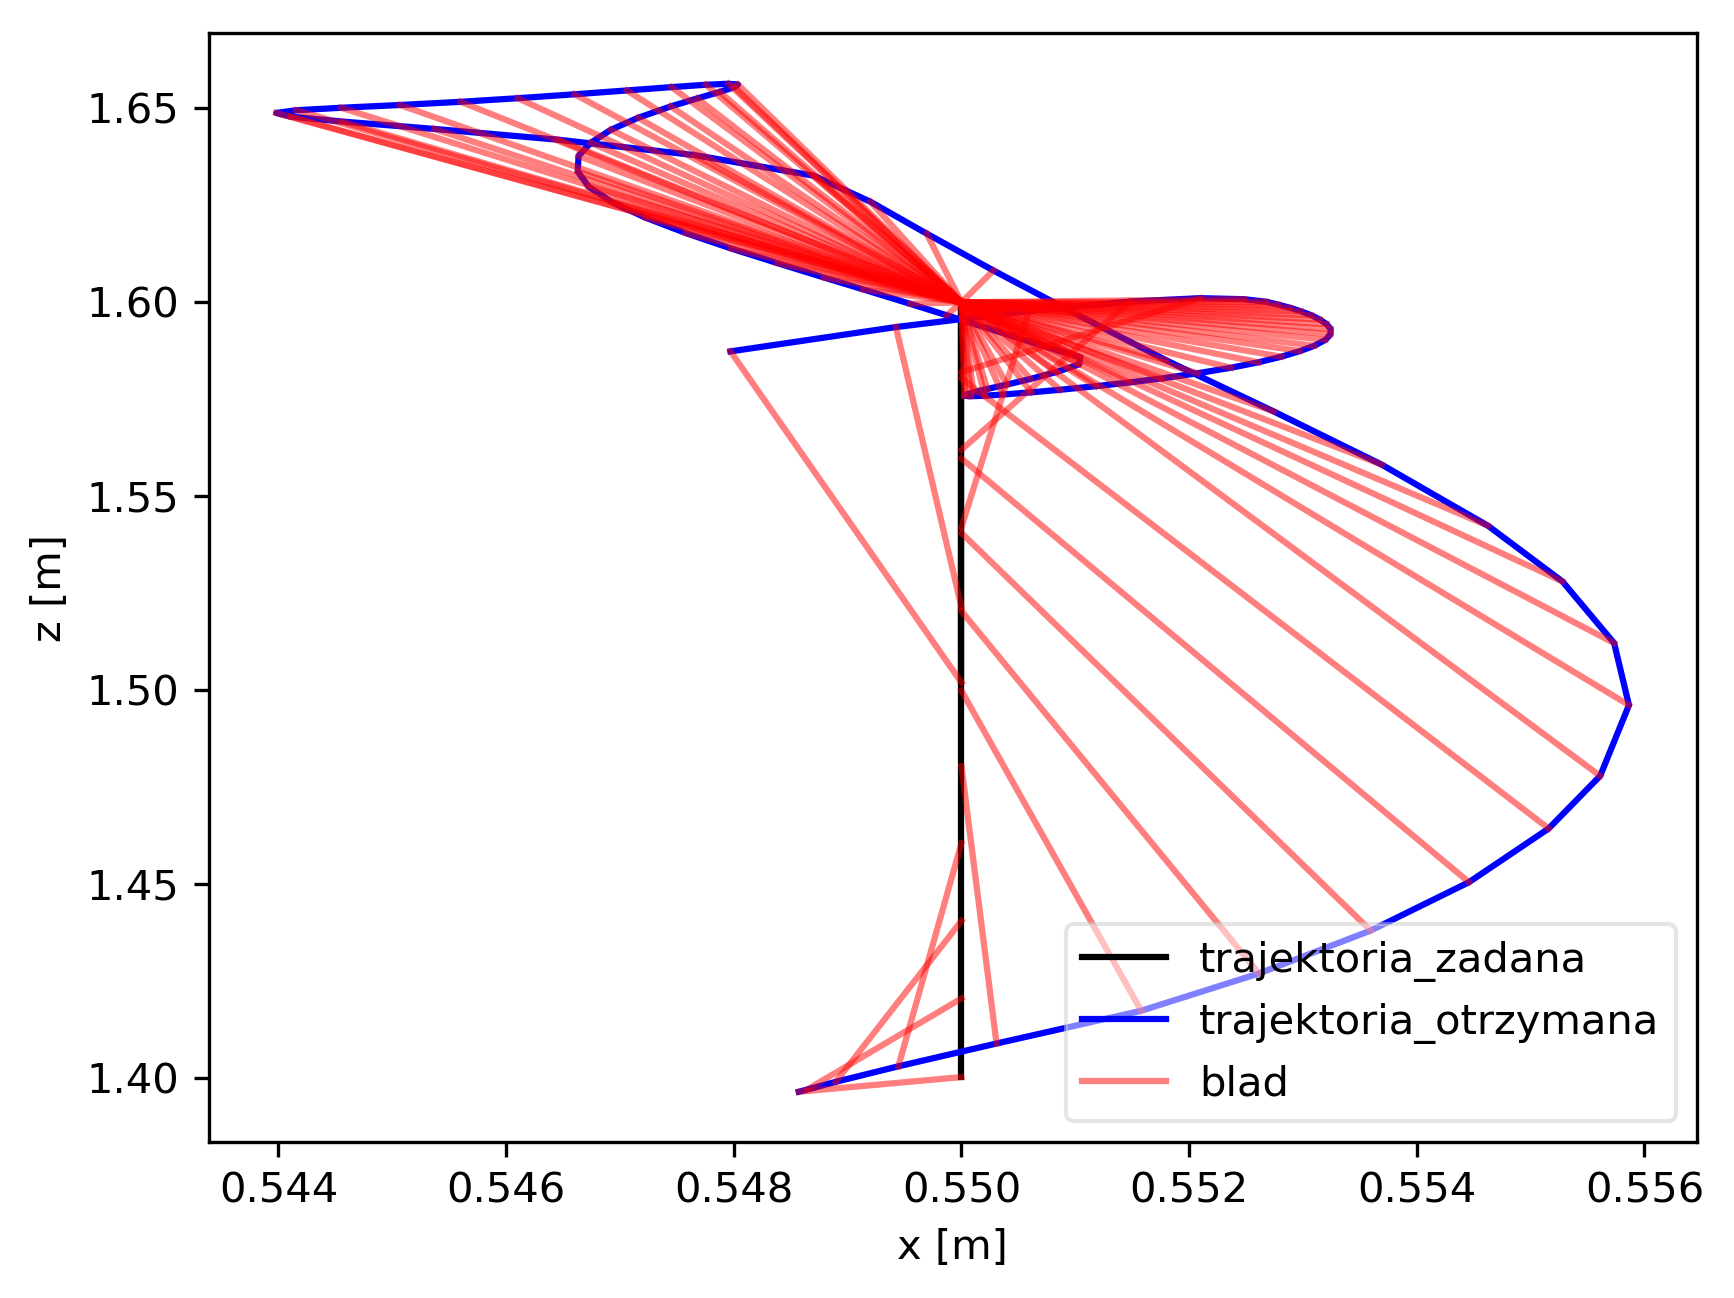
\includegraphics[width=.45\textwidth]{../../velma/przerobione_testy/out/do_gory/xz_ate_plot_podnoszenie_miekki_komp_wiertarka.png}
	}
	\caption{Porownanie trajektorii chwytaka w osiach $X$ i $Z$}
	\label{fig:do_gory_porow_przedm}
\end{figure}


% \begin{figure}
% 	\centering
% 	\subfigure[Brak algorytmu kompensacji]{
% 		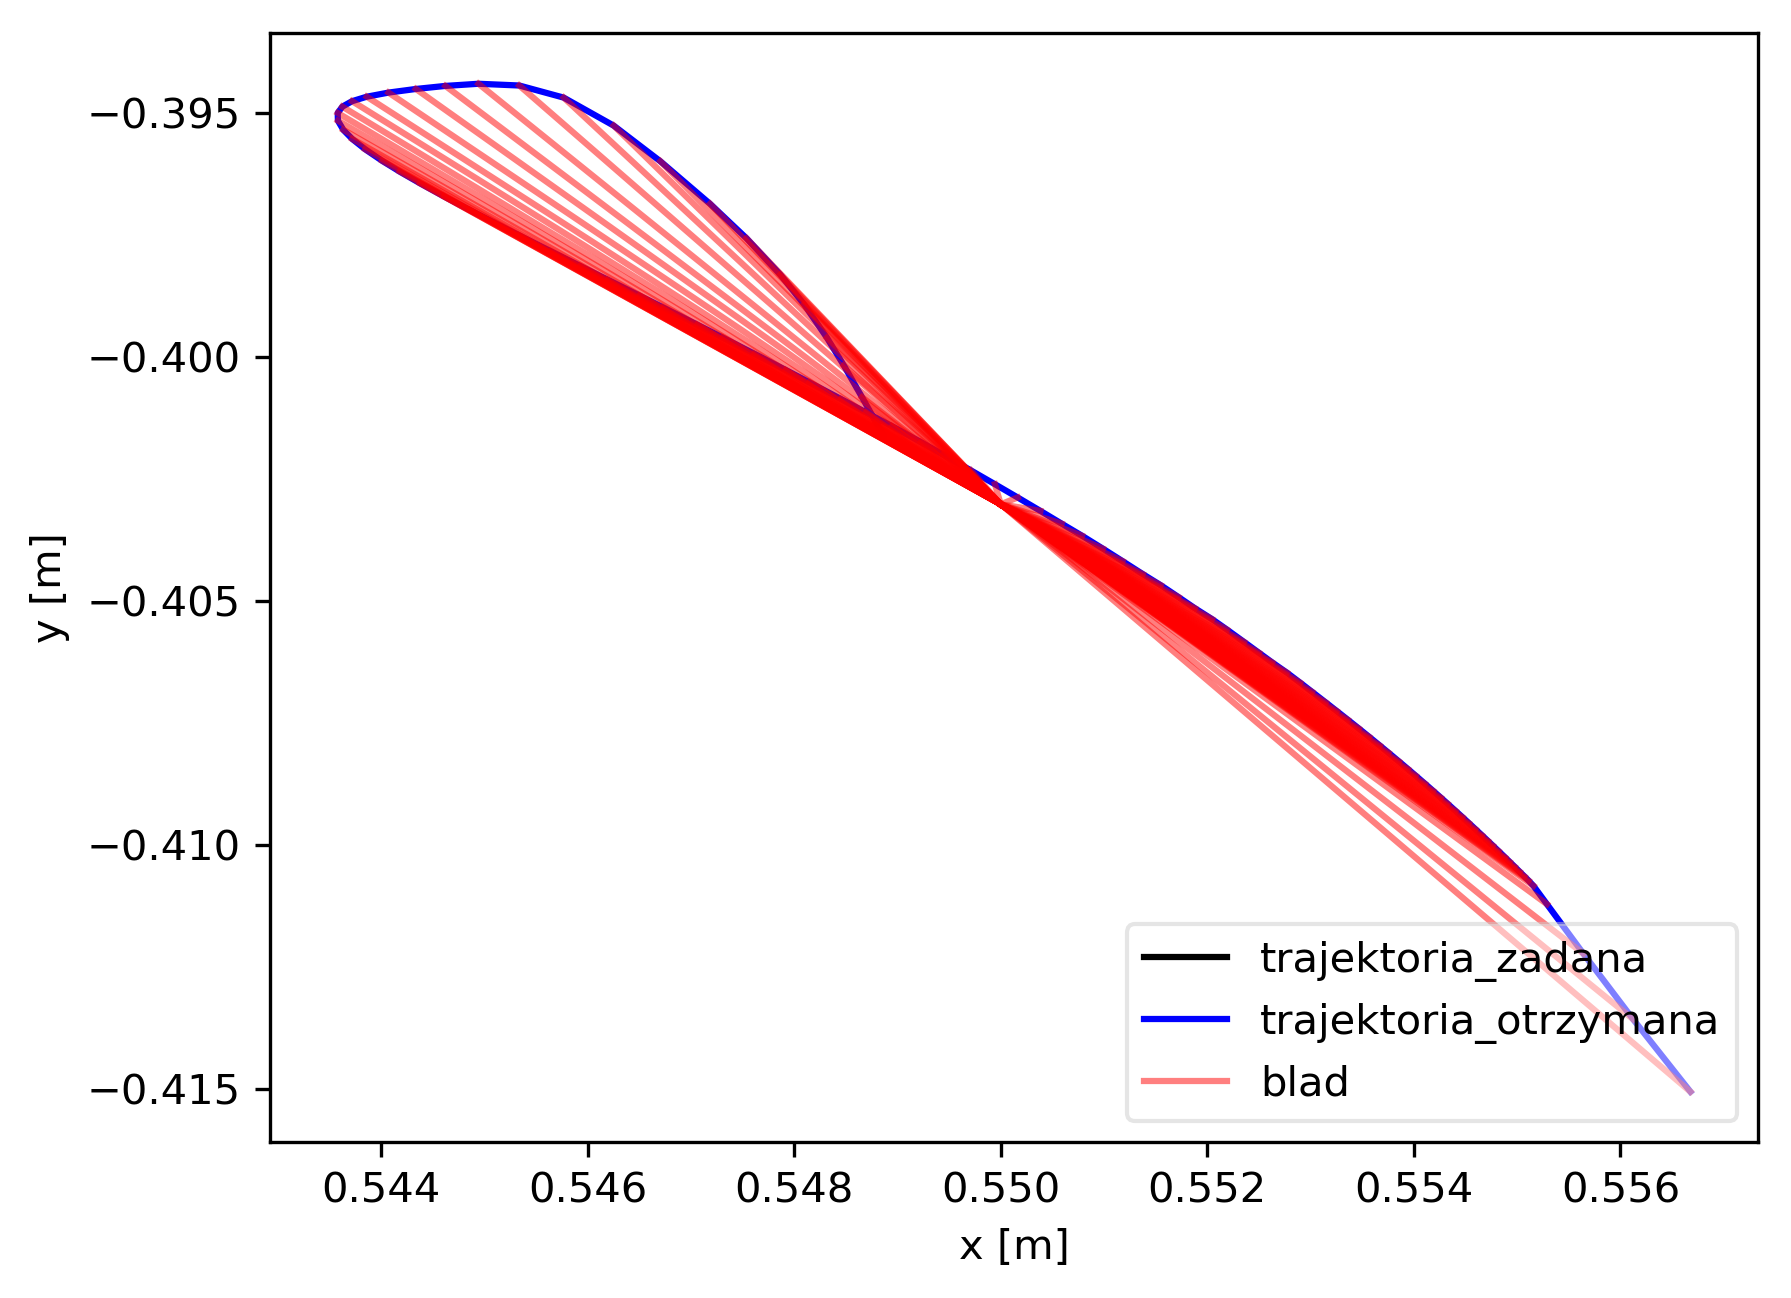
\includegraphics[width=.45\textwidth]{../../velma/przerobione_testy/out/do_gory/xy_ate_plot_podnoszenie_miekki_bez_brak.png}
% 	}
% 	\hfill
% 	\subfigure[Zalaczony algorytm kompnesacji]{
% 		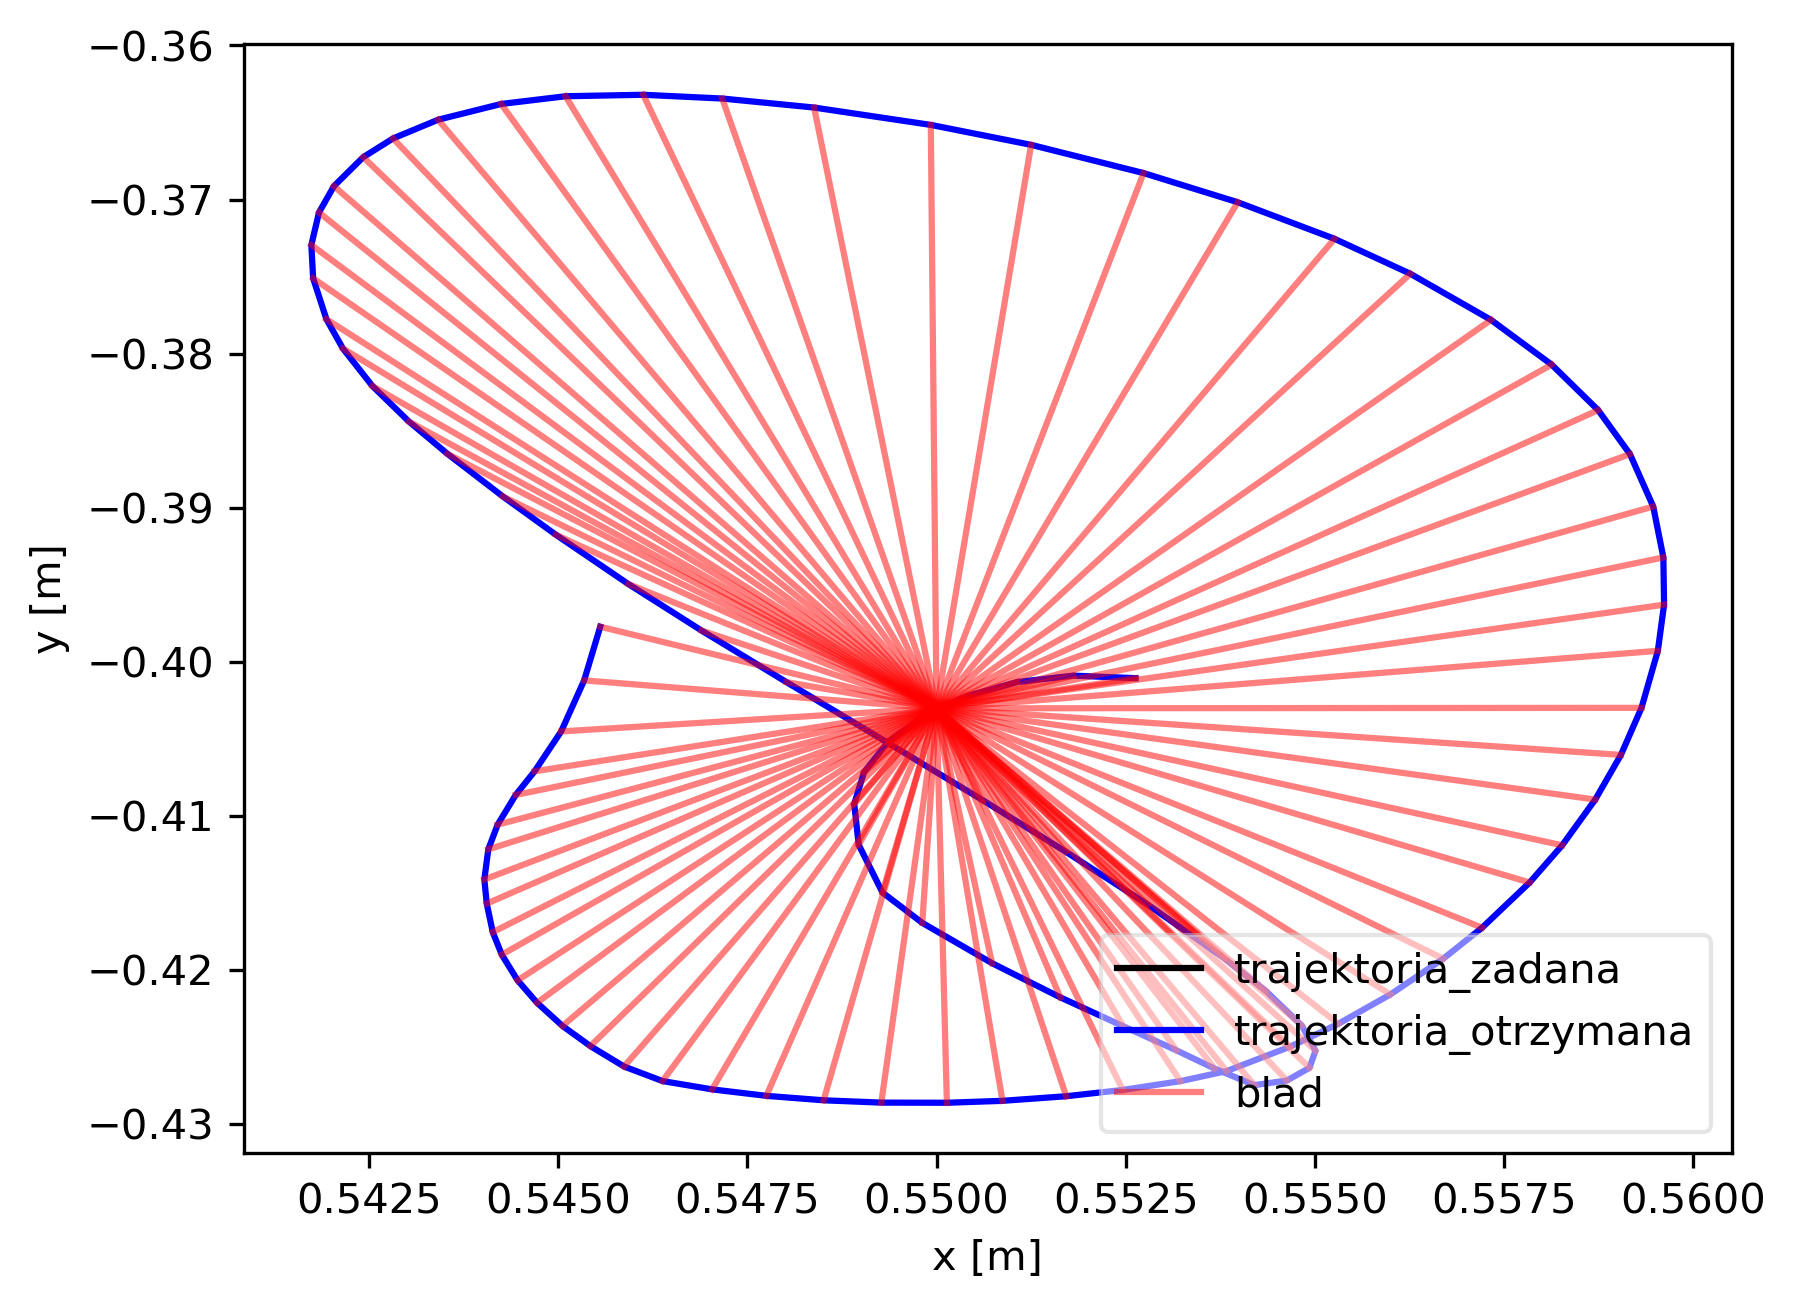
\includegraphics[width=.45\textwidth]{../../velma/przerobione_testy/out/do_gory/xy_ate_plot_podnoszenie_miekki_komp_brak.png}
% 	}
% 	\caption{Porownanie trajektorii chwytaka w osiach $X$ i $Y$}
% 	\label{fig:do_gory_porow_komp_bok}
% \end{figure}

% \begin{figure}
% 	\centering
% 	\subfigure[Trajektoria z chwycona puszka]{
% 		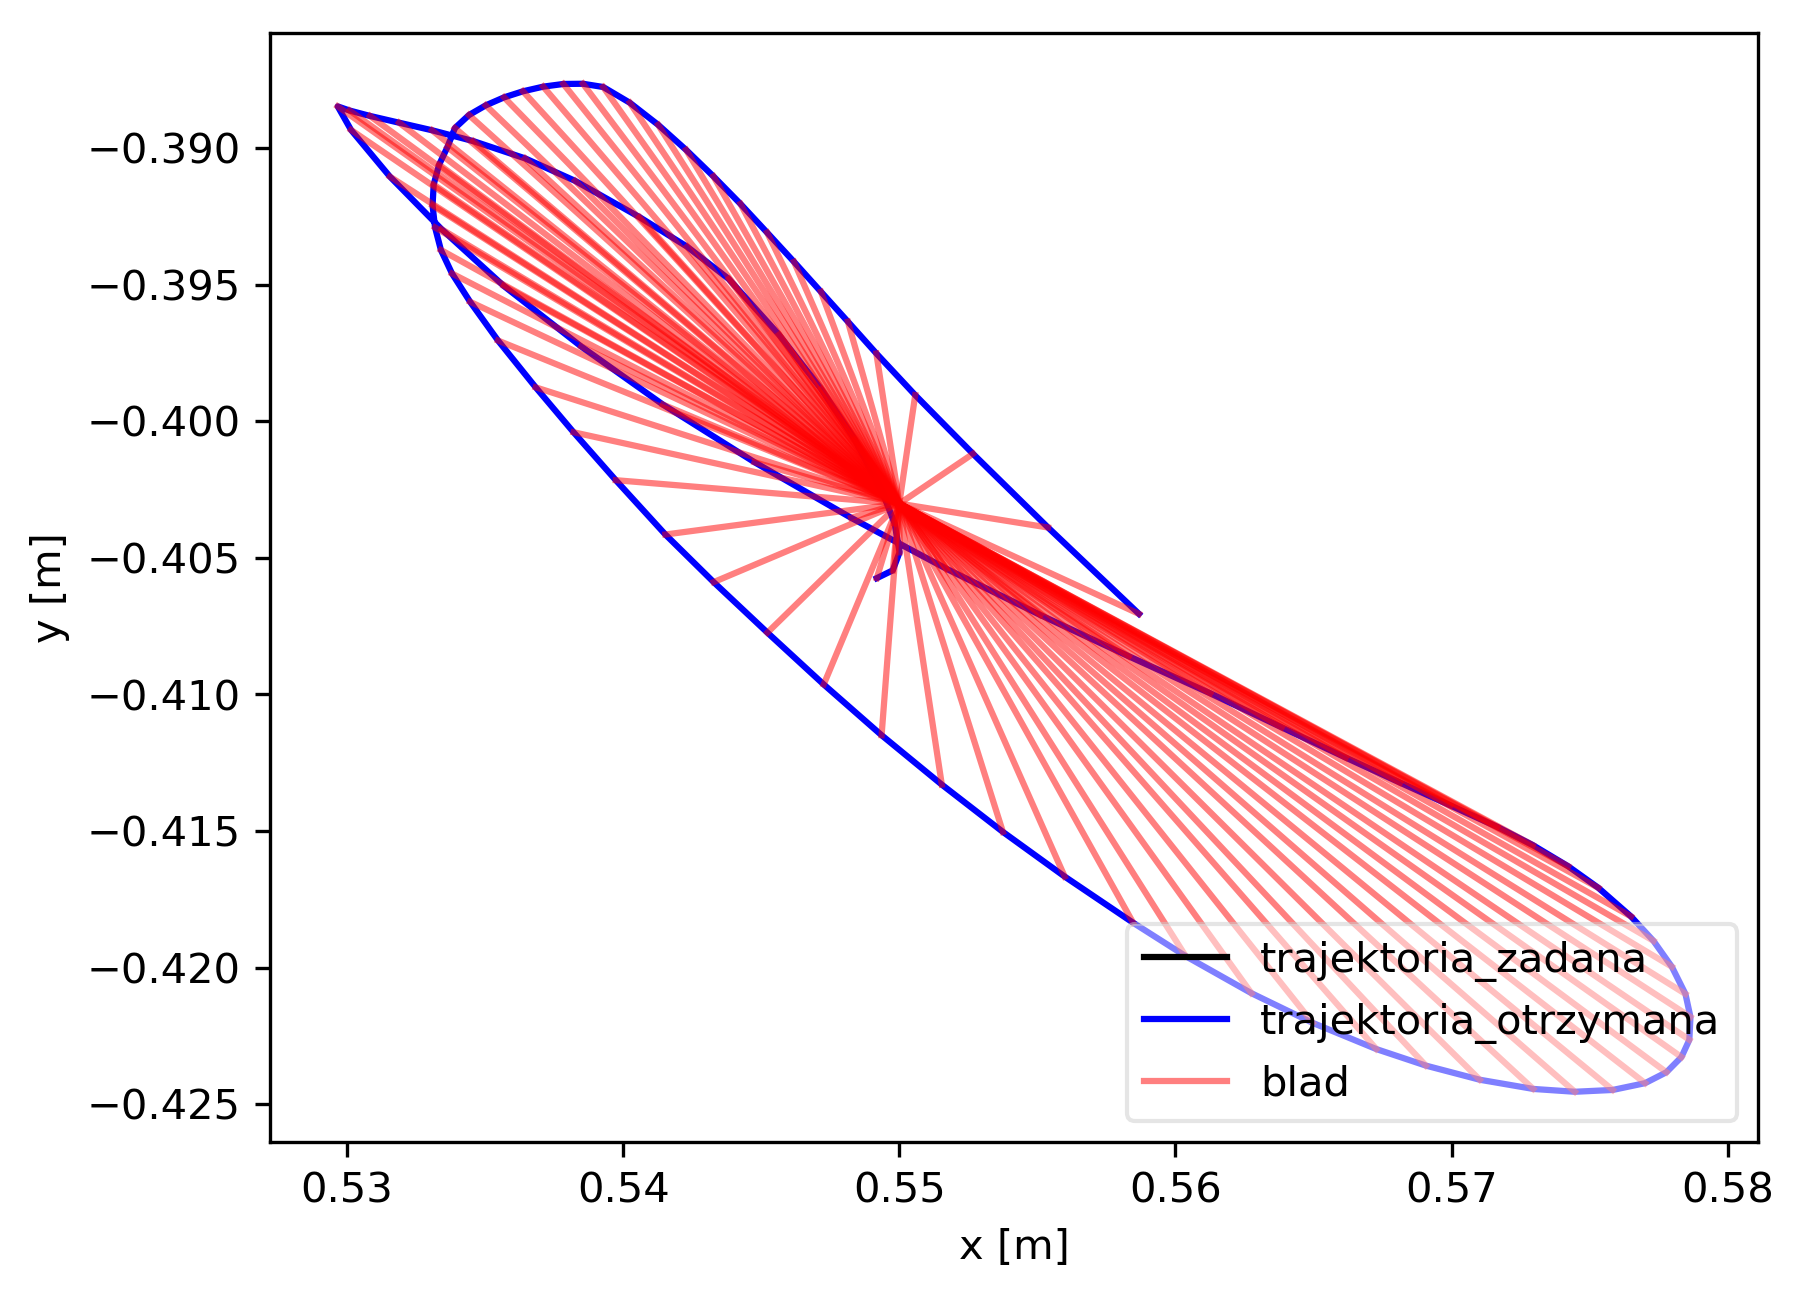
\includegraphics[width=.45\textwidth]{../../velma/przerobione_testy/out/do_gory/xy_ate_plot_podnoszenie_miekki_komp_piwo.png}
% 	}
% 	\hfill
% 	\subfigure[Trajektoria z chwycona wiertarka]{
% 		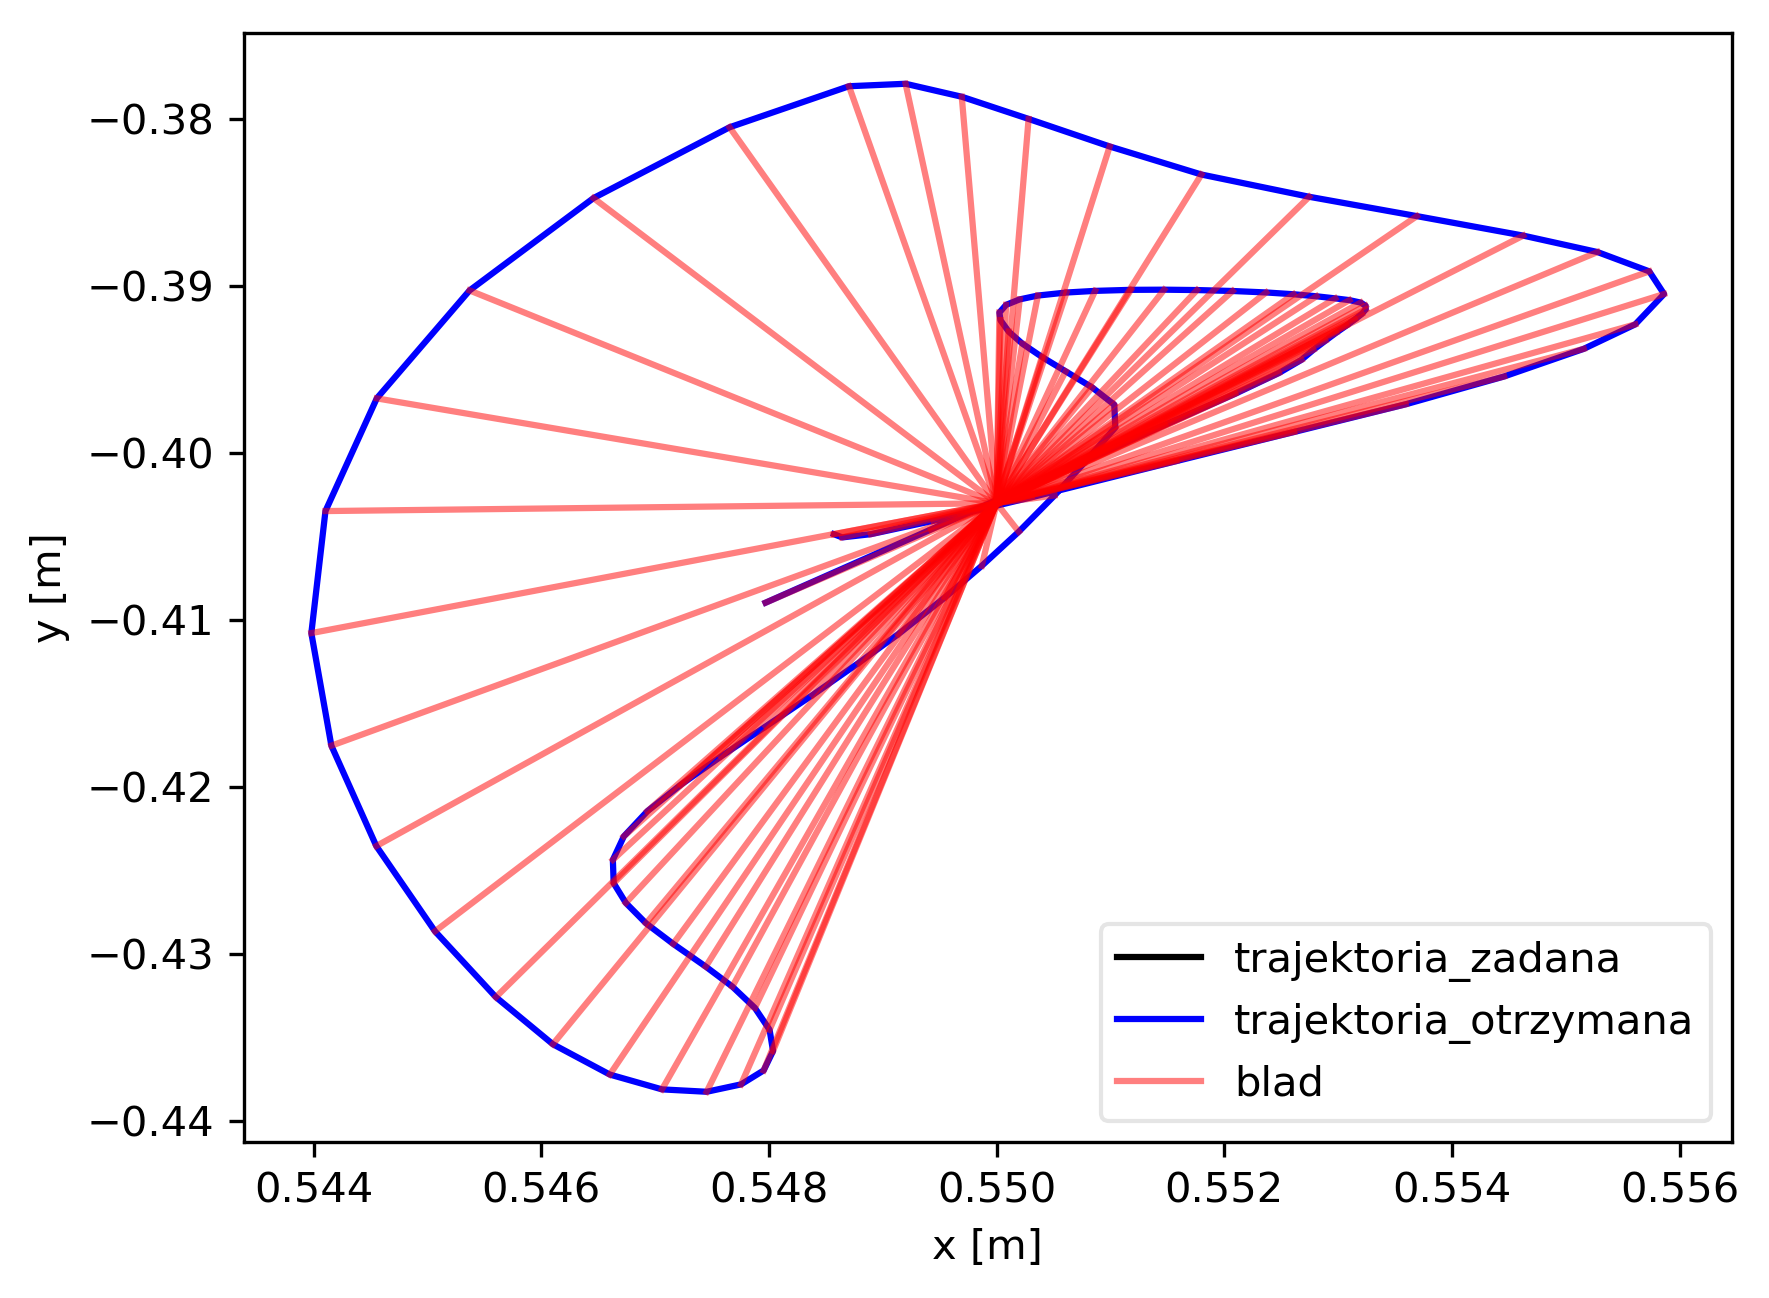
\includegraphics[width=.45\textwidth]{../../velma/przerobione_testy/out/do_gory/xy_ate_plot_podnoszenie_miekki_komp_wiertarka.png}
% 	}
% 	\caption{Porownanie trajektorii chwytaka w osiach $X$ i $Y$}
% 	\label{fig:do_gory_porow_przedm_bok}
% \end{figure}

\begin{figure}[h]
	\centering
	\subfigure[Rzut na wprost]{
		\label{fig:do_gory_porow_zbiorcze_a}
		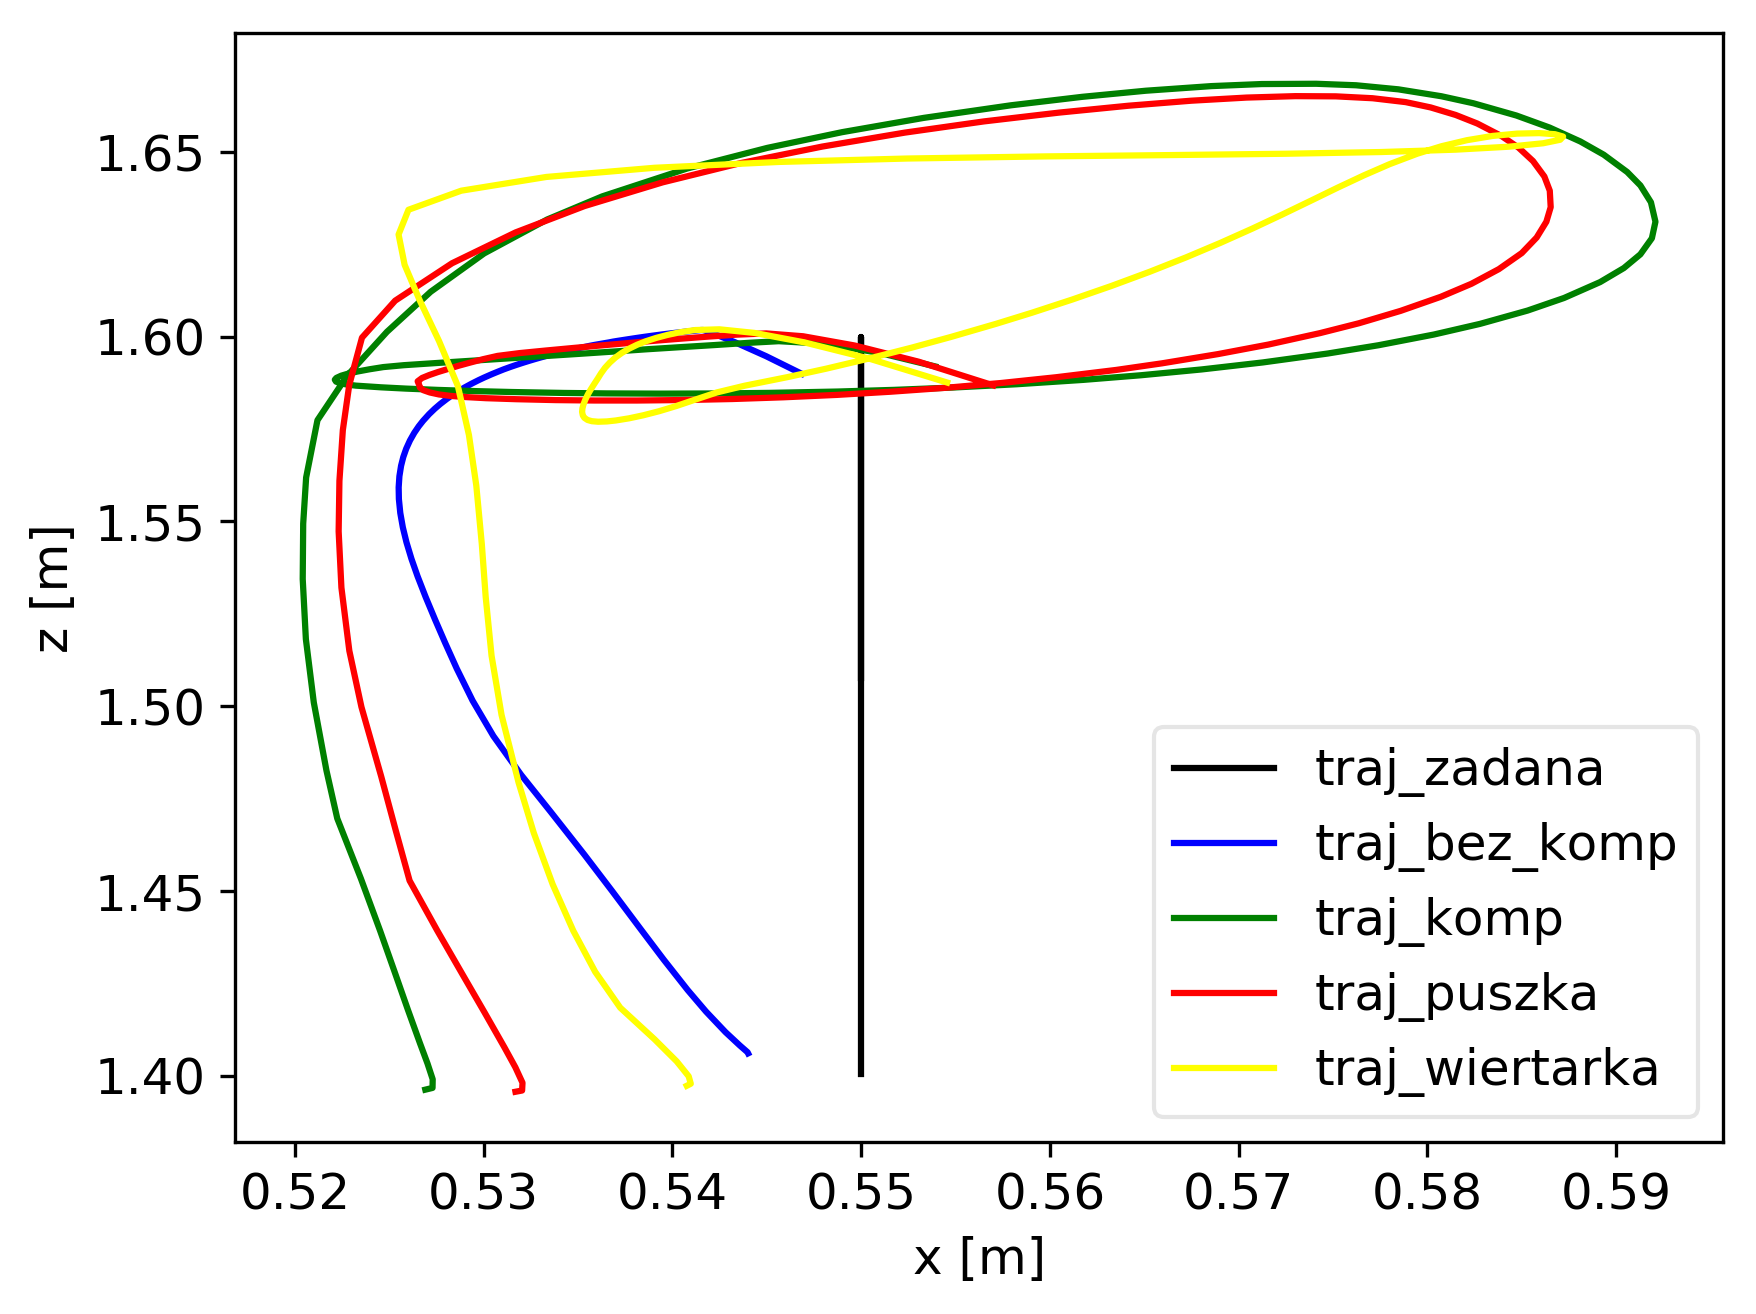
\includegraphics[width=.45\textwidth]{../../velma/przerobione_testy/out/do_gory/common_xz.png}
	}
	% \hfill
	% \subfigure[Rzut z gory]{
	% 	\label{fig:do_gory_porow_zbiorcze_b}
	% 	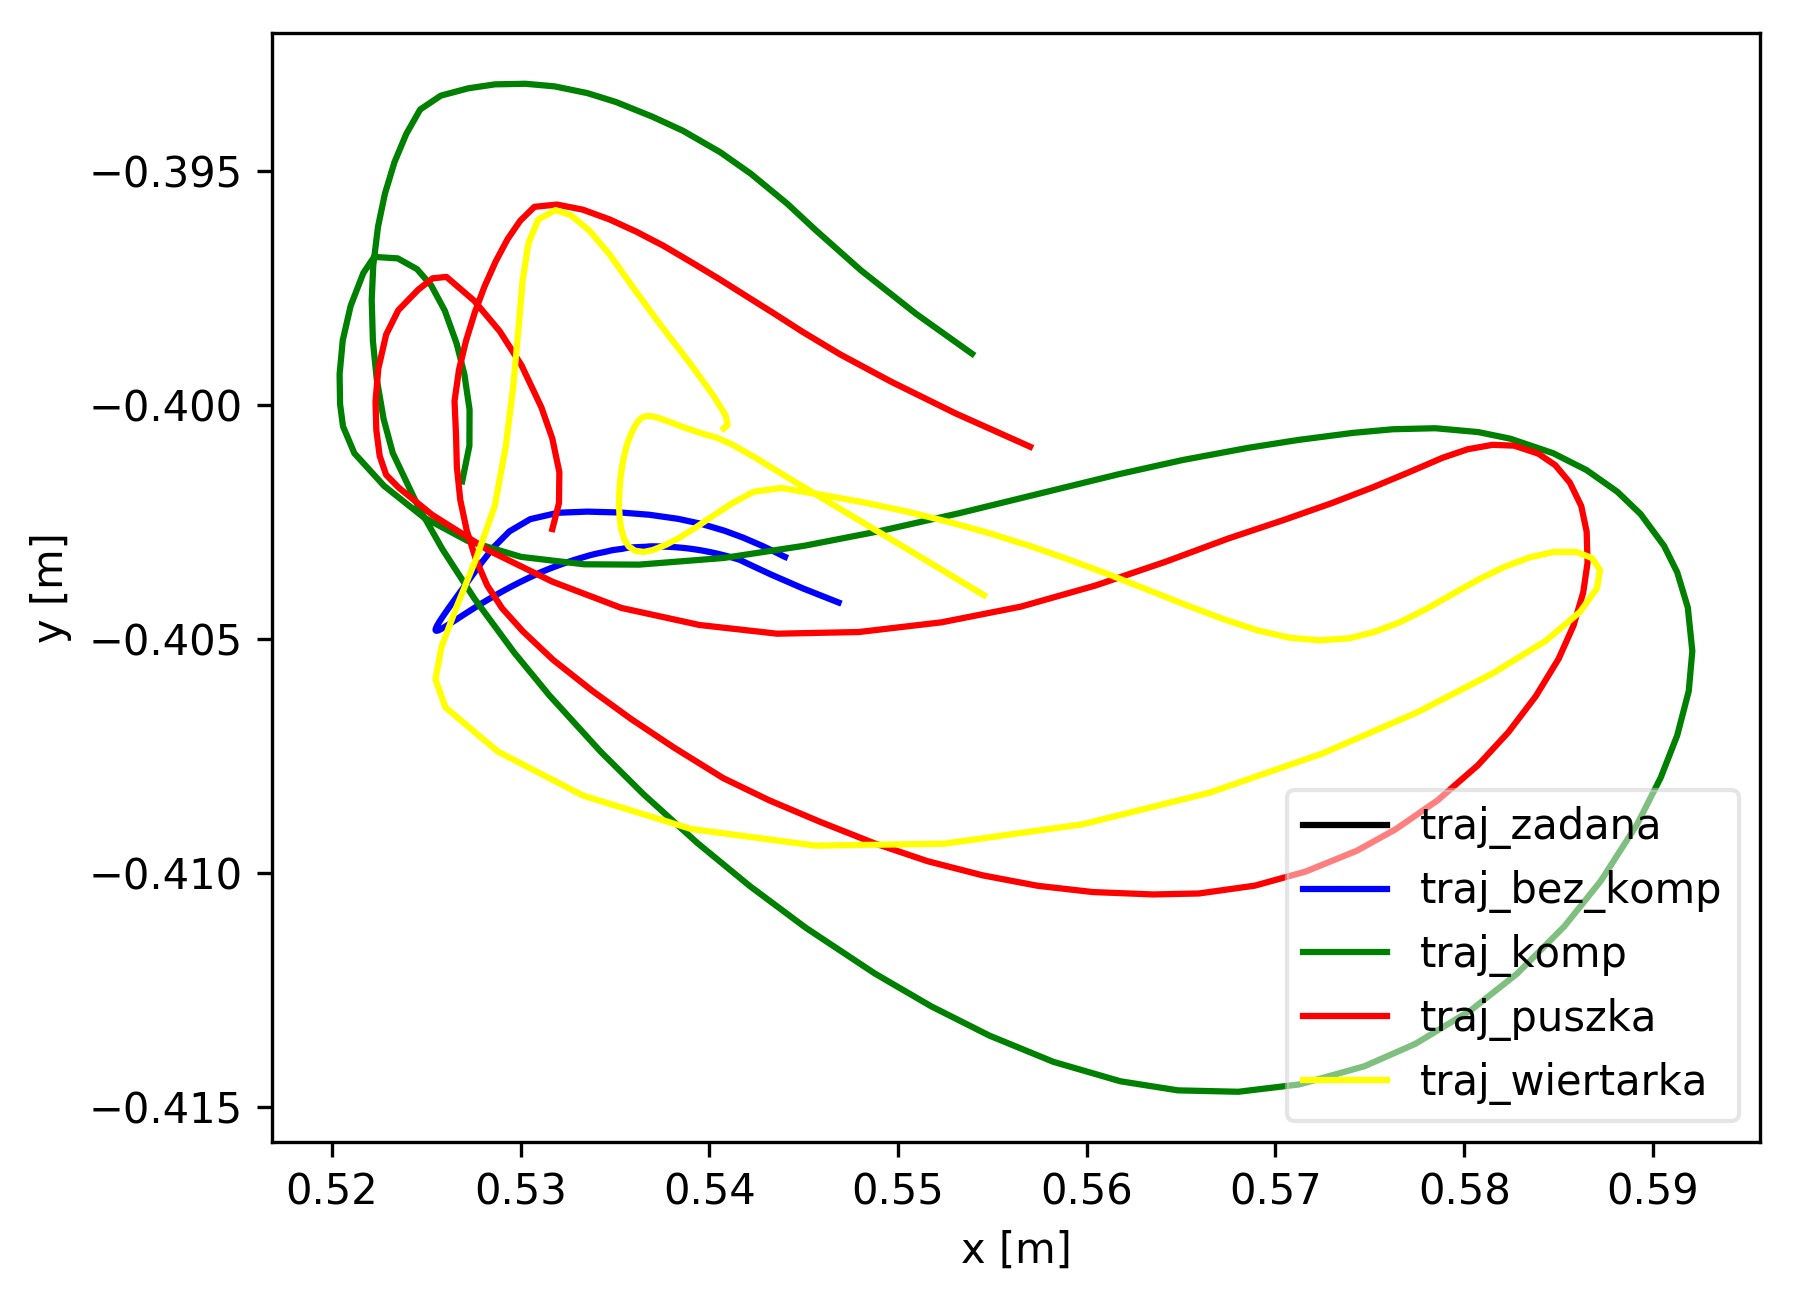
\includegraphics[width=.45\textwidth]{../../velma/przerobione_testy/out/do_gory/common_xy.png}
	% }
	\caption{Porowanie wszystkich trajektorii.}
	\label{fig:do_gory_porow_zbiorcze}
\end{figure}

\subsection{Ruch do dolu}

Eksperyment ma przetestowac zachowanie algorytmu kompensacji przy ruchu koncowki do dolu (rys. \ref{fig:do_dolu_a}, \ref{fig:do_dolu_rot}). Podobnie jak przy eksperymencie ruchu do gory warty uwagi jest aspekt dzialania sily grawitacji w tej samej co ruch osi. Trajektoria ruchu w rzucie APE na wprost ruchu zostala zaprezentowana na rys. \ref{fig:do__porow_komp}, \ref{fig:do_dolu_porow_przedm} i \ref{fig:do_dolu_porow_zbiorcze_a}. 
% Trajektoria widoczna z boku (w osiach $X$ oraz $Z$) zostala zaprezentowana na rys. \ref{fig:do_dolu_porow_komp_bok}, \ref{fig:do_dolu_porow_przedm_bok} i \ref{fig:do_dolu_porow_zbiorcze_b}.

\begin{figure}[h]
	\centering
	\subfigure[Os $X$]{
		\label{fig:do_dolu_ax}
		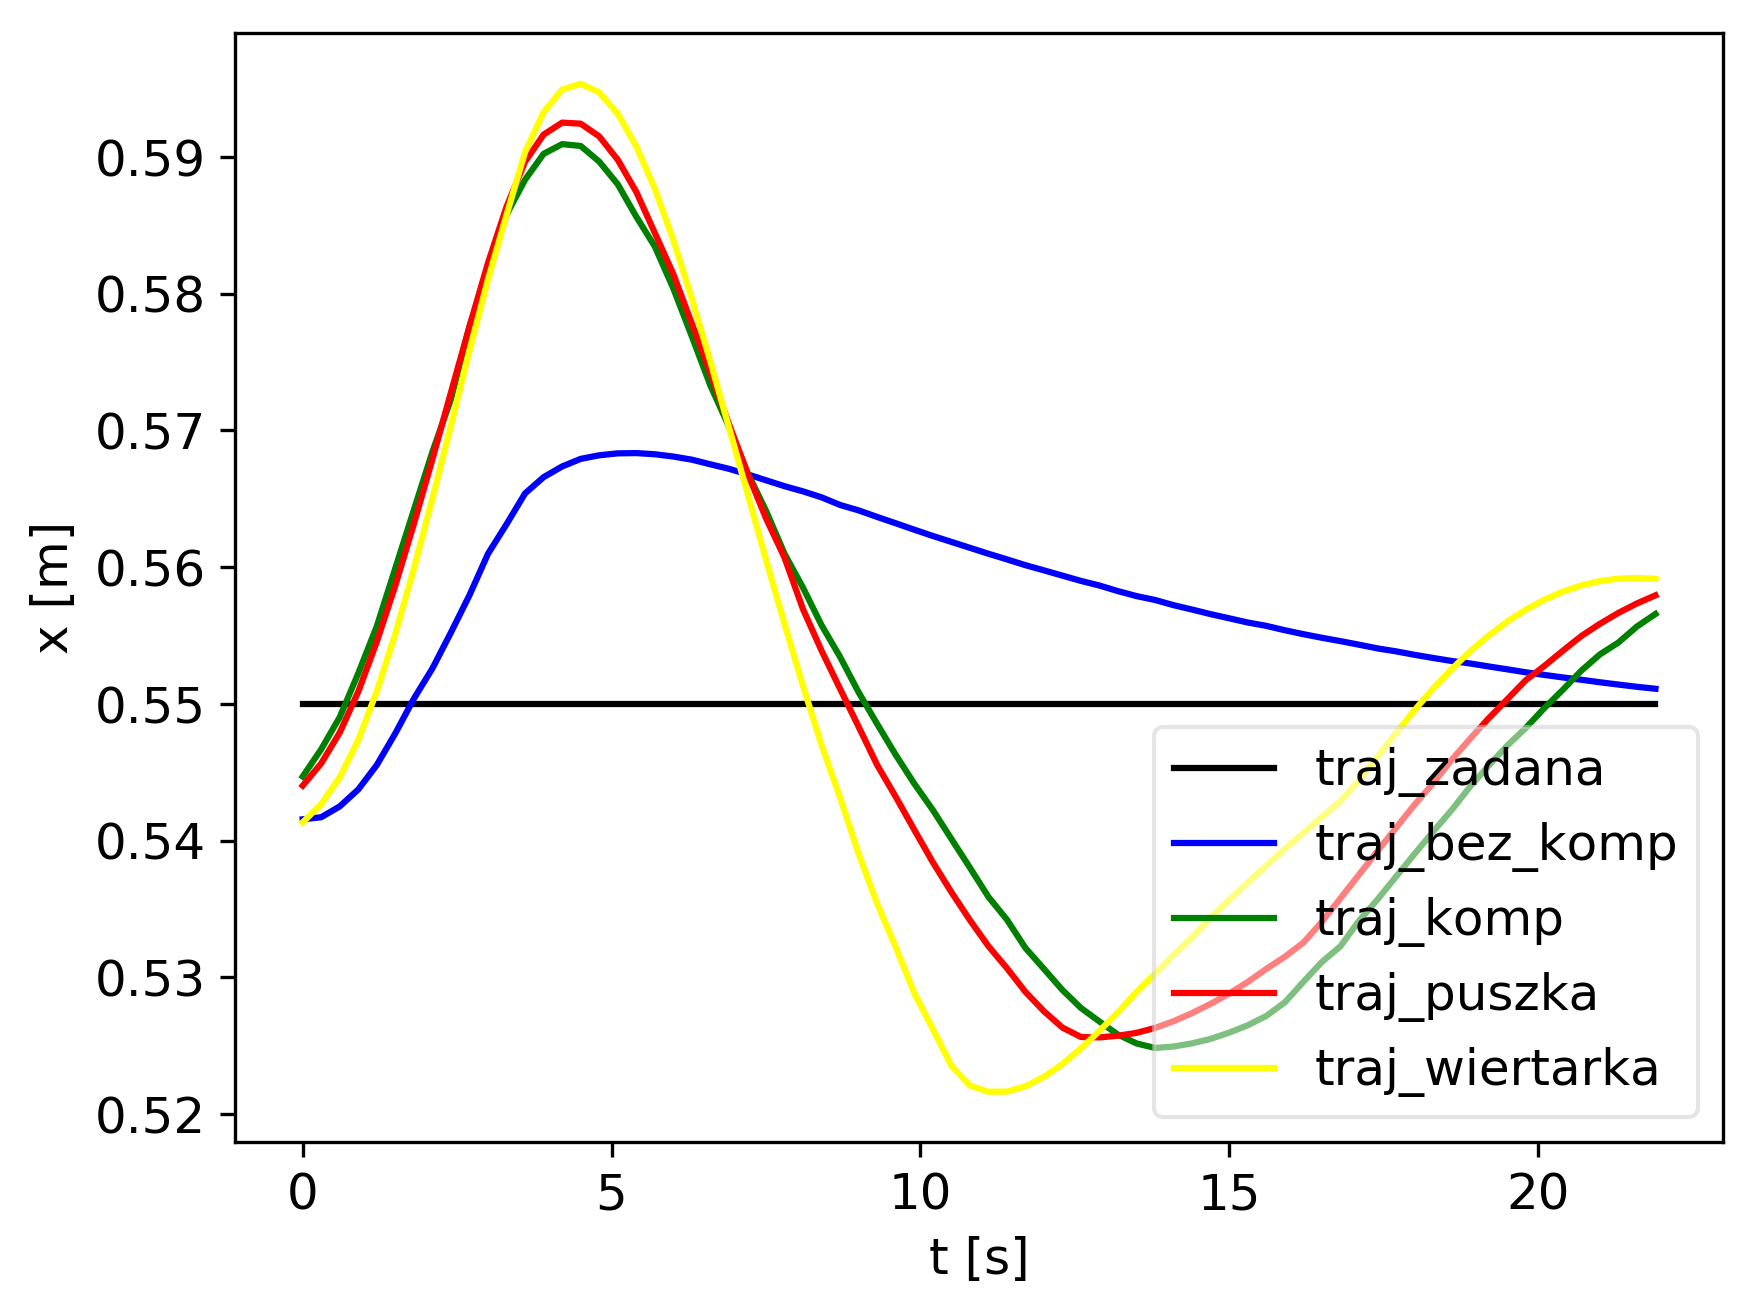
\includegraphics[width=.45\textwidth]{../../velma/przerobione_testy/out/do_dolu/common_ax.png}
	}
	\hfill
	\subfigure[Os $Y$]{
		\label{fig:do_dolu_ay}
		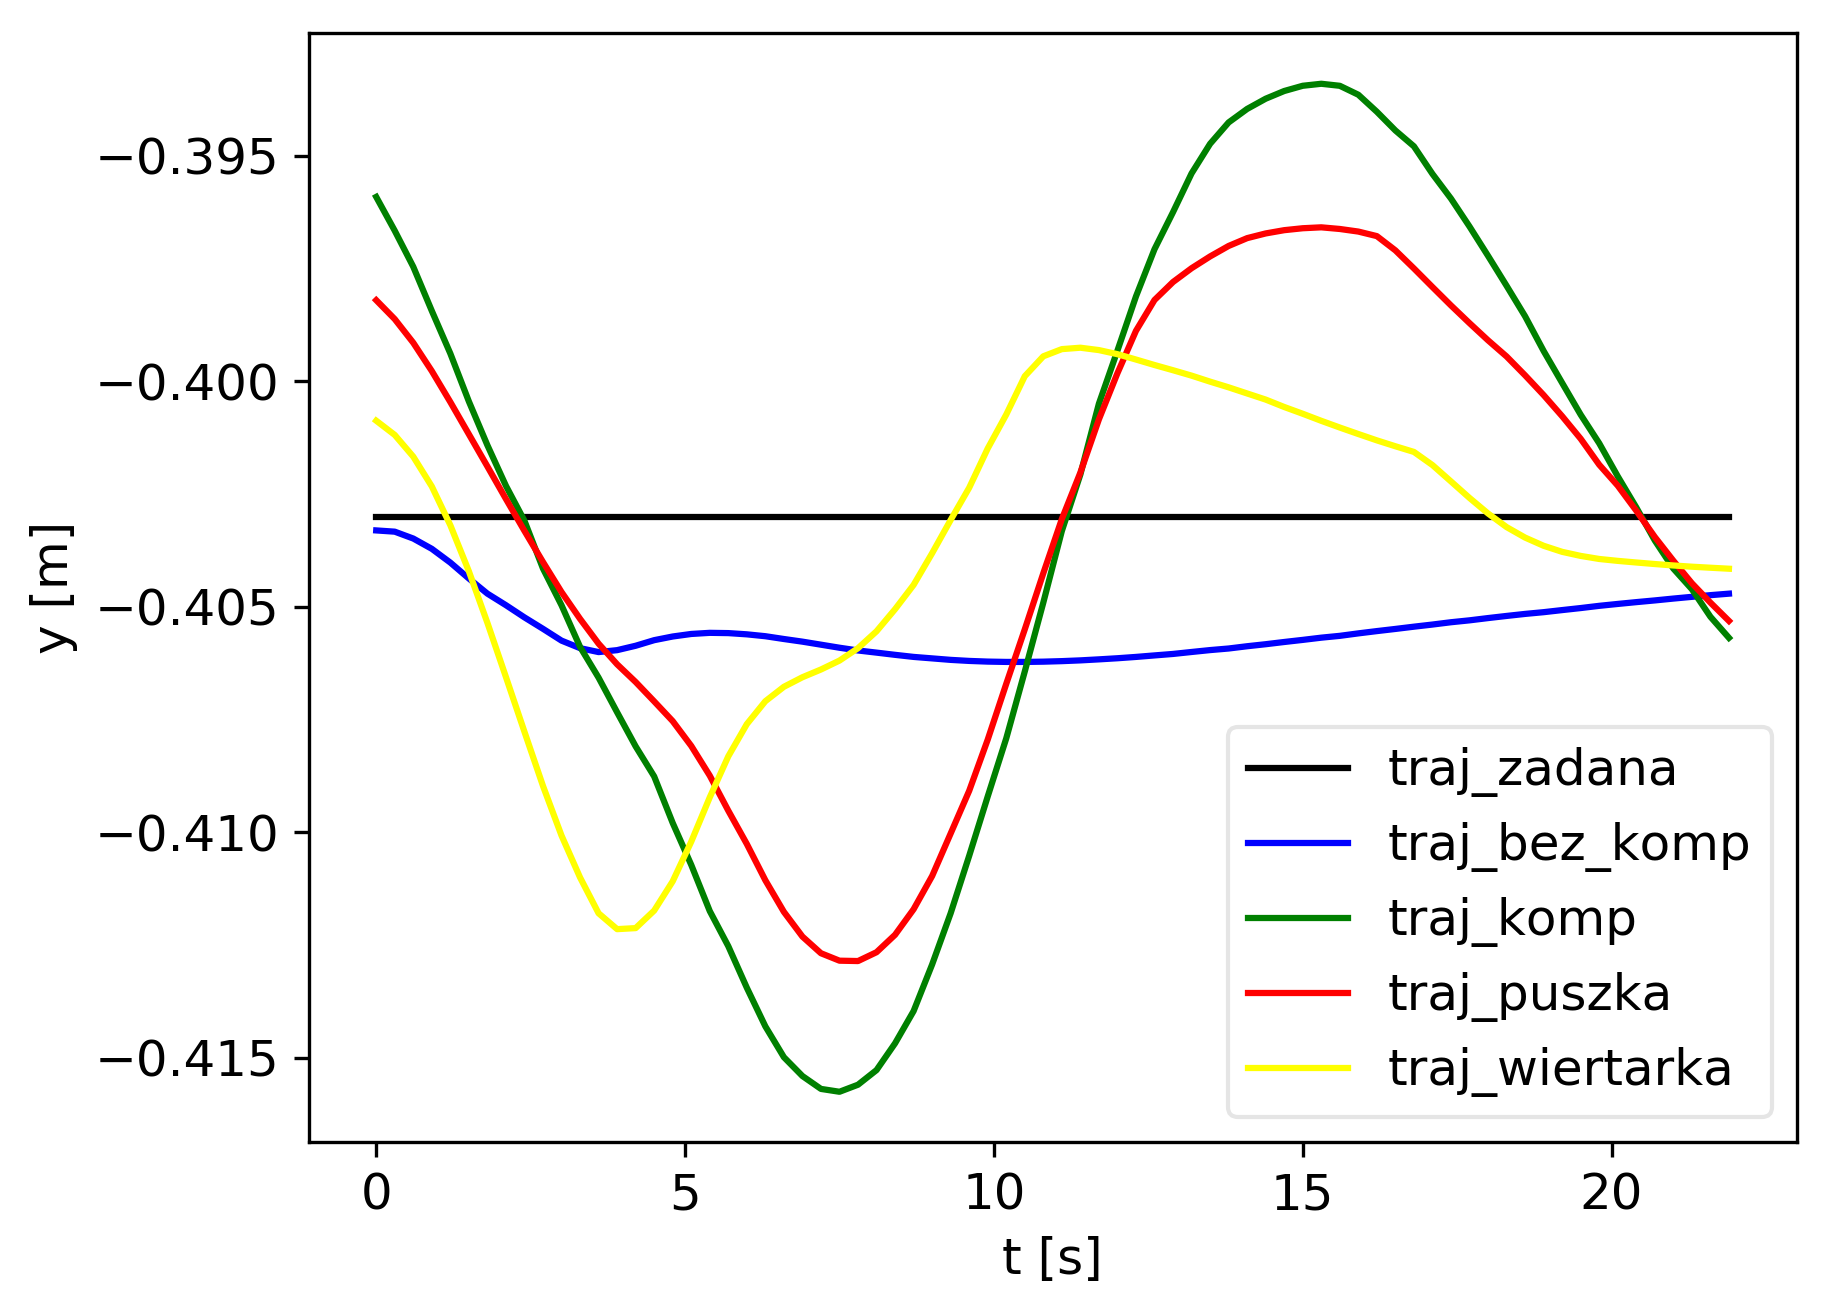
\includegraphics[width=.45\textwidth]{../../velma/przerobione_testy/out/do_dolu/common_ay.png}
	}
	
	\hfill
	\subfigure[Os $Z$]{
		\label{fig:do_dolu_az}
		\includegraphics[width=.45\textwidth]{../../velma/przerobione_testy/out/do_dolu/common_az.png}
	}

	\caption{Ruch do dolu. Porownanie trajektorii pozycji w zaleznosci od czasu.}
	\label{fig:do_dolu_a}

\end{figure}


\begin{figure}[h]
	\centering
	\subfigure[Kat osi $X$]{
		\label{fig:do_dolu_rotx}
		\includegraphics[width=.45\textwidth]{../../velma/przerobione_testy/out/do_dolu/common_rotx.png}
	}
	\hfill
	\subfigure[Kat osi $Y$]{
		\label{fig:do_dolu_roty}
		\includegraphics[width=.45\textwidth]{../../velma/przerobione_testy/out/do_dolu/common_roty.png}
	}
	
	\hfill
	\subfigure[Kat osi $Z$]{
		\label{fig:do_dolu_rotz}
		\includegraphics[width=.45\textwidth]{../../velma/przerobione_testy/out/do_dolu/common_rotz.png}
	}

	\caption{Ruch do dolu. Porownanie trajektorii katow w notacji Eulera w zaleznosci od czasu.}
	\label{fig:do_dolu_rot}

\end{figure}


\begin{figure}[h]
	\centering
	\subfigure[Brak algorytmu kompensacji]{
		\includegraphics[width=.45\textwidth]{../../velma/przerobione_testy/out/do_dolu/xz_ate_plot_podnoszenie_miekki_bez_brak.png}
	}
	\hfill
	\subfigure[Zalaczony algorytm kompnesacji]{
		\includegraphics[width=.45\textwidth]{../../velma/przerobione_testy/out/do_dolu/xz_ate_plot_podnoszenie_miekki_komp_brak.png}
	}
	\caption{Porownanie trajektorii chwytaka w osiach $X$ i $Z$}
	\label{fig:do_dolu_porow_komp}
\end{figure}

\begin{figure}[h]
	\centering
	\subfigure[Trajektoria z chwycona puszka]{
		\includegraphics[width=.45\textwidth]{../../velma/przerobione_testy/out/do_dolu/xz_ate_plot_podnoszenie_miekki_komp_piwo.png}
	}
	\hfill
	\subfigure[Trajektoria z chwycona wiertarka]{
		\includegraphics[width=.45\textwidth]{../../velma/przerobione_testy/out/do_dolu/xz_ate_plot_podnoszenie_miekki_komp_wiertarka.png}
	}
	\caption{Porownanie trajektorii chwytaka w osiach $X$ i $Z$}
	\label{fig:do_dolu_porow_przedm}
\end{figure}


% \begin{figure}
% 	\centering
% 	\subfigure[Brak algorytmu kompensacji]{
% 		\includegraphics[width=.45\textwidth]{../../velma/przerobione_testy/out/do_dolu/xy_ate_plot_podnoszenie_miekki_bez_brak.png}
% 	}
% 	\hfill
% 	\subfigure[Zalaczony algorytm kompnesacji]{
% 		\includegraphics[width=.45\textwidth]{../../velma/przerobione_testy/out/do_dolu/xy_ate_plot_podnoszenie_miekki_komp_brak.png}
% 	}
% 	\caption{Porownanie trajektorii chwytaka w osiach $X$ i $Y$}
% 	\label{fig:do_dolu_porow_komp_bok}
% \end{figure}

% \begin{figure}
% 	\centering
% 	\subfigure[Trajektoria z chwycona puszka]{
% 		\includegraphics[width=.45\textwidth]{../../velma/przerobione_testy/out/do_dolu/xy_ate_plot_podnoszenie_miekki_komp_piwo.png}
% 	}
% 	\hfill
% 	\subfigure[Trajektoria z chwycona wiertarka]{
% 		\includegraphics[width=.45\textwidth]{../../velma/przerobione_testy/out/do_dolu/xy_ate_plot_podnoszenie_miekki_komp_wiertarka.png}
% 	}
% 	\caption{Porownanie trajektorii chwytaka w osiach $X$ i $Y$}
% 	\label{fig:do_dolu_porow_przedm_bok}
% \end{figure}

\begin{figure}[h]
	\centering
	\subfigure[Rzut na wprost]{
		\label{fig:do_dolu_porow_zbiorcze_a}
		\includegraphics[width=.45\textwidth]{../../velma/przerobione_testy/out/do_dolu/common_xz.png}
	}
	\hfill
	% \subfigure[Rzut z gory]{
	% 	\label{fig:do_dolu_porow_zbiorcze_b}
	% 	\includegraphics[width=.45\textwidth]{../../velma/przerobione_testy/out/do_dolu/common_xy.png}
	% }
	\caption{Porowanie wszystkich trajektorii.}
	\label{fig:do_dolu_porow_zbiorcze}
\end{figure}

\subsection{Ruch do przodu}

Eksperyment ma przetestowac zachowanie algorytmu kompensacji przy ruchu koncowki w kierunku od robota (rys. \ref{fig:do_przodu_a}, \ref{fig:do_przodu_rot}). Trajektoria ruchu w rzucie na wprost ruchu zostala zaprezentowana na rys. \ref{fig:do_przodu_porow_komp}, \ref{fig:do_przodu_porow_przedm} i \ref{fig:do_przodu_porow_zbiorcze_a}. Trajektoria widoczna z boku (w osiach $X$ oraz $Z$) zostala zaprezentowana na rys. \ref{fig:do_przodu_porow_komp_bok}, \ref{fig:do_przodu_porow_przedm_bok} i \ref{fig:do_przodu_porow_zbiorcze_b}.

\begin{figure}
	\centering
	\subfigure[Os $X$]{
		\label{fig:do_przodu_ax}
		\includegraphics[width=.45\textwidth]{../../velma/przerobione_testy/out/do_przodu/common_ax.png}
	}
	\hfill
	\subfigure[Os $Y$]{
		\label{fig:do_przodu_ay}
		\includegraphics[width=.45\textwidth]{../../velma/przerobione_testy/out/do_przodu/common_ay.png}
	}
	
	\hfill
	\subfigure[Os $Z$]{
		\label{fig:do_przodu_az}
		\includegraphics[width=.45\textwidth]{../../velma/przerobione_testy/out/do_przodu/common_az.png}
	}

	\caption{Ruch do przodu. Porownanie trajektorii pozycji w zaleznosci od czasu.}
	\label{fig:do_przodu_a}

\end{figure}


\begin{figure}
	\centering
	\subfigure[Kat osi $X$]{
		\label{fig:do_przodu_rotx}
		\includegraphics[width=.45\textwidth]{../../velma/przerobione_testy/out/do_przodu/common_rotx.png}
	}
	\hfill
	\subfigure[Kat osi $Y$]{
		\label{fig:do_przodu_roty}
		\includegraphics[width=.45\textwidth]{../../velma/przerobione_testy/out/do_przodu/common_roty.png}
	}
	
	\hfill
	\subfigure[Kat osi $Z$]{
		\label{fig:do_przodu_rotz}
		\includegraphics[width=.45\textwidth]{../../velma/przerobione_testy/out/do_przodu/common_rotz.png}
	}

	\caption{Ruch do przodu. Porownanie trajektorii katow w notacji Eulera w zaleznosci od czasu.}
	\label{fig:do_przodu_rot}

\end{figure}


\begin{figure}
	\centering
	\subfigure[Brak algorytmu kompensacji]{
		\includegraphics[width=.45\textwidth]{../../velma/przerobione_testy/out/do_przodu/xz_ate_plot_podnoszenie_miekki_bez_brak.png}
	}
	\hfill
	\subfigure[Zalaczony algorytm kompnesacji]{
		\includegraphics[width=.45\textwidth]{../../velma/przerobione_testy/out/do_przodu/xz_ate_plot_podnoszenie_miekki_komp_brak.png}
	}
	\caption{Ruch do przodu. Porownanie trajektorii chwytaka w osiach $X$ i $Z$}
	\label{fig:do_przodu_porow_komp}
\end{figure}

\begin{figure}
	\centering
	\subfigure[Trajektoria z chwycona puszka]{
		\includegraphics[width=.45\textwidth]{../../velma/przerobione_testy/out/do_przodu/xz_ate_plot_podnoszenie_miekki_komp_piwo.png}
	}
	\hfill
	\subfigure[Trajektoria z chwycona wiertarka]{
		\includegraphics[width=.45\textwidth]{../../velma/przerobione_testy/out/do_przodu/xz_ate_plot_podnoszenie_miekki_komp_wiertarka.png}
	}
	\caption{Ruch do przodu. Porownanie trajektorii chwytaka w osiach $X$ i $Z$}
	\label{fig:do_przodu_porow_przedm}
\end{figure}


\begin{figure}
	\centering
	\subfigure[Brak algorytmu kompensacji]{
		\includegraphics[width=.45\textwidth]{../../velma/przerobione_testy/out/do_przodu/xy_ate_plot_podnoszenie_miekki_bez_brak.png}
	}
	\hfill
	\subfigure[Zalaczony algorytm kompnesacji]{
		\includegraphics[width=.45\textwidth]{../../velma/przerobione_testy/out/do_przodu/xy_ate_plot_podnoszenie_miekki_komp_brak.png}
	}
	\caption{Porownanie trajektorii chwytaka w osiach $X$ i $Y$}
	\label{fig:do_przodu_porow_komp_bok}
\end{figure}

\begin{figure}
	\centering
	\subfigure[Trajektoria z chwycona puszka]{
		\includegraphics[width=.45\textwidth]{../../velma/przerobione_testy/out/do_przodu/xy_ate_plot_podnoszenie_miekki_komp_piwo.png}
	}
	\hfill
	\subfigure[Trajektoria z chwycona wiertarka]{
		\includegraphics[width=.45\textwidth]{../../velma/przerobione_testy/out/do_przodu/xy_ate_plot_podnoszenie_miekki_komp_wiertarka.png}
	}
	\caption{Porownanie trajektorii chwytaka w osiach $X$ i $Y$}
	\label{fig:do_przodu_porow_przedm_bok}
\end{figure}

\begin{figure}
	\centering
	\subfigure[Rzut na wprost]{
		\label{fig:do_przodu_porow_zbiorcze_a}
		\includegraphics[width=.45\textwidth]{../../velma/przerobione_testy/out/do_przodu/common_xz.png}
	}
	\hfill
	\subfigure[Rzut z gory]{
		\label{fig:do_przodu_porow_zbiorcze_b}
		\includegraphics[width=.45\textwidth]{../../velma/przerobione_testy/out/do_przodu/common_xy.png}
	}
	\caption{Porowanie wszystkich trajektorii bez zaznaczonego bledu.}
	\label{fig:do_przodu_porow_zbiorcze}
\end{figure}


\subsection{Obrot koncowki}

Eksperyment ma przetestowac zachowanie algorytmu kompensacji przy obrocie koncowki. Obserwacje polegaja na zmianie polozen katowych koncowki bez zmiany pozycji. Koncowka ma obrocic sie o zadany kat we wszystkich osiach (rys.\ref{fig:obrt_a}, \ref{fig:obrt_rot}) Trajektoria ruchu (w osiach $X$ oraz $Y$) zostala zaprezentowana na rys. \ref{fig:obrt_porow_komp}, \ref{fig:obrt_porow_przedm} i \ref{fig:obrt_porow_zbiorcze_a}. Trajektoria widoczna z boku (w osiach $X$ oraz $Z$) zostala zaprezentowana na rys. \ref{fig:obrt_porow_komp_bok}, \ref{fig:obrt_porow_przedm_bok} i \ref{fig:obrt_porow_zbiorcze_b}.

\begin{figure}
	\centering
	\subfigure[Os $X$]{
		\label{fig:obrt_ax}
		\includegraphics[width=.45\textwidth]{../../velma/przerobione_testy/out/obrt/common_ax.png}
	}
	\hfill
	\subfigure[Os $Y$]{
		\label{fig:obrt_ay}
		\includegraphics[width=.45\textwidth]{../../velma/przerobione_testy/out/obrt/common_ay.png}
	}
	
	\hfill
	\subfigure[Os $Z$]{
		\label{fig:obrt_az}
		\includegraphics[width=.45\textwidth]{../../velma/przerobione_testy/out/obrt/common_az.png}
	}

	\caption{Porownanie trajektorii pozycji w zaleznosci od czasu.}
	\label{fig:obrt_a}

\end{figure}


\begin{figure}
	\centering
	\subfigure[Kat osi $X$]{
		\label{fig:obrt_rotx}
		\includegraphics[width=.45\textwidth]{../../velma/przerobione_testy/out/obrt/common_rotx.png}
	}
	\hfill
	\subfigure[Kat osi $Y$]{
		\label{fig:obrt_roty}
		\includegraphics[width=.45\textwidth]{../../velma/przerobione_testy/out/obrt/common_roty.png}
	}
	
	\hfill
	\subfigure[Kat osi $Z$]{
		\label{fig:obrt_rotz}
		\includegraphics[width=.45\textwidth]{../../velma/przerobione_testy/out/obrt/common_rotz.png}
	}

	\caption{Porownanie trajektorii katow w notacji Eulera w zaleznosci od czasu.}
	\label{fig:obrt_rot}

\end{figure}


\begin{figure}
	\centering
	\subfigure[Brak algorytmu kompensacji]{
		\includegraphics[width=.45\textwidth]{../../velma/przerobione_testy/out/obrt/xz_ate_plot_podnoszenie_miekki_bez_brak.png}
	}
	\hfill
	\subfigure[Zalaczony algorytm kompnesacji]{
		\includegraphics[width=.45\textwidth]{../../velma/przerobione_testy/out/obrt/xz_ate_plot_podnoszenie_miekki_komp_brak.png}
	}
	\caption{Porownanie trajektorii chwytaka w osiach $X$ i $Z$}
	\label{fig:obrt_porow_komp}
\end{figure}

\begin{figure}
	\centering
	\subfigure[Trajektoria z chwycona puszka]{
		\includegraphics[width=.45\textwidth]{../../velma/przerobione_testy/out/obrt/xz_ate_plot_podnoszenie_miekki_komp_piwo.png}
	}
	\hfill
	\subfigure[Trajektoria z chwycona wiertarka]{
		\includegraphics[width=.45\textwidth]{../../velma/przerobione_testy/out/obrt/xz_ate_plot_podnoszenie_miekki_komp_wiertarka.png}
	}
	\caption{Porownanie trajektorii chwytaka w osiach $X$ i $Z$}
	\label{fig:obrt_porow_przedm}
\end{figure}


\begin{figure}
	\centering
	\subfigure[Brak algorytmu kompensacji]{
		\includegraphics[width=.45\textwidth]{../../velma/przerobione_testy/out/obrt/xy_ate_plot_podnoszenie_miekki_bez_brak.png}
	}
	\hfill
	\subfigure[Zalaczony algorytm kompnesacji]{
		\includegraphics[width=.45\textwidth]{../../velma/przerobione_testy/out/obrt/xy_ate_plot_podnoszenie_miekki_komp_brak.png}
	}
	\caption{Porownanie trajektorii chwytaka w osiach $X$ i $Y$}
	\label{fig:obrt_porow_komp_bok}
\end{figure}

\begin{figure}
	\centering
	\subfigure[Trajektoria z chwycona puszka]{
		\includegraphics[width=.45\textwidth]{../../velma/przerobione_testy/out/obrt/xy_ate_plot_podnoszenie_miekki_komp_piwo.png}
	}
	\hfill
	\subfigure[Trajektoria z chwycona wiertarka]{
		\includegraphics[width=.45\textwidth]{../../velma/przerobione_testy/out/obrt/xy_ate_plot_podnoszenie_miekki_komp_wiertarka.png}
	}
	\caption{Porownanie trajektorii chwytaka w osiach $X$ i $Y$}
	\label{fig:obrt_porow_przedm_bok}
\end{figure}

\begin{figure}
	\centering
	\subfigure[Rzut na wprost]{
		\label{fig:obrt_porow_zbiorcze_a}
		\includegraphics[width=.45\textwidth]{../../velma/przerobione_testy/out/obrt/common_xz.png}
	}
	\hfill
	\subfigure[Rzut z gory]{
		\label{fig:obrt_porow_zbiorcze_b}
		\includegraphics[width=.45\textwidth]{../../velma/przerobione_testy/out/obrt/common_xy.png}
	}
	\caption{Porowanie wszystkich trajektorii bez zaznaczonego bledu.}
	\label{fig:obrt_porow_zbiorcze}
\end{figure}

\begin{figure}
	\centering
	\subfigure[Trajektoria z chwycona puszka]{
		\includegraphics[width=.45\textwidth]{../../velma/przerobione_testy/out/obrt/xy_ate_plot_podnoszenie_miekki_komp_piwo.png}
	}
	\hfill
	\subfigure[Trajektoria z chwycona wiertarka]{
		\includegraphics[width=.45\textwidth]{../../velma/przerobione_testy/out/obrt/xy_ate_plot_podnoszenie_miekki_komp_wiertarka.png}
	}
	\caption{Porownanie trajektorii chwytaka w osiach $X$ i $Y$}
	\label{fig:obrt_porow_przedm_bok}
\end{figure}



\subsection{Ocena jakosci kolizji}
Ocena jakosci kolizji nastepuje poprzez przylozenie skokowych momentow do stawow ramienia oraz obserwacji zachowania robota. Ocena jakosci uginania robota pod wplywem  symulowanej kolizji nastepuje zgodnie z metoda opisana w sekcji \ref{chap:ocenakonaktu}.

\subsection{Podsumowanie}